% -*- Document-Type: LaTeX; Master-File: manual.tex -*- 
% Date de creation: [ck: Aug  8 95][ck: Jul  9 96]

\listfiles

\documentclass[11pt]{book}
\usepackage{graphics,epsfig,makeidx,latexsym,fancyhead,supertabular}
\usepackage{lgrind} \LGnuminterval=1

% Pour la generation de pdf avec liens (table des matieres et bibliographie)
% Ne sert que lorsque pdflatex est utilise
\usepackage{hyperref}


%\batchmode

\pagestyle{plain}

        \marginparwidth 0pt 
        \oddsidemargin 0pt 
        \evensidemargin 0pt 
        \marginparsep 0pt
        \topmargin -5mm 
        \textwidth 160mm 
        \textheight 235mm

%%%%%%%%%%%%%%%% CE QUI DEPEND DE LA VERSION %%%%%%%%%%%%%%%%%%%%%
\newcommand{\versionElan}{V3.6}
\newcommand{\elanVersion}{\versionElan}
\newcommand{\localisationFtpElan}{{\tt /pub/loria/protheo/softwares/Elan/elan.3.6.tgz}}
\newcommand{\localisationWebElan}{{\tt http://elan.loria.fr}}
%%%%%%%%%%%%%%%% DECLARATION D'ORTHOGRAPHE!%%%%%%%%%%%%%%%%%%%%%%%
% L'orthographe du document est basee sur l'usage Americain
%%%%%%%%%%%%%%%%

% Les macros
% [ck: Feb  7 89]
% les macros speciales pour le livre

%%%%%%%% traitement des exercices a la Knuth:
%%%%% 1. le fichier de reponses et le compteur
\newwrite\ans
\immediate\openout\ans=reponses
\newcount\exno\global\exno=0
% 2. la macro de definition de l'enonce
\chardef\other=12
\newcommand{\exercice}[1]
   {\global\advance\exno by 1 
    {\small\noindent {\bf Exercice~\the\exno~---} #1}\ifvmode\else\newline\fi
   }
%%%%% 3.  la macros de definition de la reponse
% fait avec Eric [ck: Aug 20 93]
\outer\def\answer{\par\medbreak
  \immediate\write\ans{}
  \immediate\write\ans{\the\exno:}
  \copytoblankline}
\def\copytoblankline{\begingroup\setupcopy\copyans}
\def\setupcopy{\def\do##1{\catcode`##1=\other}\dospecials
  \catcode`\|=\other \obeylines}
{\obeylines \gdef\copyans#1
  {\def\next{#1}%
  \ifx\next\empty\let\next=\endgroup %
  \else\immediate\write\ans{\next} \let\next=\copyans\fi\next}}

%%%%% 4. Utiliser les reponses en chantant dans l'annexe A
%    \immediate\closeout\ans \input{reponses}
%%%%% 5. Utilisation typique
%       \exercice{enonce'}
%       \answer{reponse eventuelle (non obligatoire)}
%              <- ligne blanche OBLIGATOIRE apres la reponse
%                 Attention aux lignes blanches dans la reponse!
%%%%% 6. Ancienne macro
\newcommand{\exer}[2]{\global\advance\exno by 1 
    {\small\noindent {\bf Exercice~\the\exno~---} #1}\ifvmode\else\newline\fi
     }          %%%%%%% \noindent{\bf Answer}: #2}
%%%%%%%%%%%%%%%%%%%%%%%%%%%%%%%%%%%%%%%%%%%%%%%%%%%%%%%%%%%%%%%%
\newcommand{\coq}{\textsf{Coq}}
\newcommand{\elan}{\textsf{ELAN}}
\let\ELAN=\elan
\newcommand{\REF}{\textsf{REF}}

% Lecture supplementaires: Further Readings
\newcommand{\FR}[1]{\noindent{\it Further Readings: #1}}

% attention passage dangereux
\newcommand{\zz}{$\bigodot$}

\newcommand{\Helene}{H{\'e}l{\`e}ne}

% Impression d'un passage en deux colonnes
% attention a la separation des colonnes et a leur largeur

\newcommand{\deuxcol}[2]{
        \noindent
        \begin{minipage}[t]{5.5cm}
        #1
        \end{minipage} \ ~~~ \
        \begin{minipage}[t]{5.5cm}
        #2
        \end{minipage}
        }

 % pour traiter les theories equationnelles introduites dans le livre
 % et faire un index specifique des theo equa
\newcommand{\thname}[1]{\index{#1|sfac}{\sf #1}}
\newcommand{\trsname}[1]{\overrightarrow{\sf #1}} 

% pour les fleches longues une abbrev:
\newcommand{\vect}[1]{\overrightarrow{#1}}

\newcommand{\bold}[1]{{\bf #1}}
\newcommand{\ital}[1]{{\it #1}}
\newcommand{\sfac}[1]{{\sf #1}}

\newcommand{\ul}[1]{\underline{#1}}
\newcommand{\ol}[1]{\overline{#1}}

\newcommand{\subsubsubsection}[1]{{\sc #1 \break}}
\newcommand{\DEF}{\begin{definition}\begin{rm}}
\newcommand{\FDEF}{\end{rm}\end{definition}}
\newcommand{\PROP}{\begin{proposition}\begin{rm}}
\newcommand{\FPROP}{\end{rm}\end{proposition}}
\newcommand{\COR}{\begin{corollary}\begin{rm}}
\newcommand{\FCOR}{\end{rm}\end{corollary}}
\newcommand{\EX}{\begin{example}\begin{rm}}
\newcommand{\FEX}{\end{rm}\end{example}}
\renewcommand{\TH}{\begin{theorem}}
\newcommand{\FTH}{\end{theorem}}
\newcommand{\LEM}{\begin{lemma}\begin{rm}}
\newcommand{\FLEM}{\end{rm}\end{lemma}}

\newcommand{\Def}[1]{{\em #1}\index{#1}} % |bold}}
\newcommand{\Aut}[1]{{#1}\index{#1|ital}}
        % typiquement pour indexer les auteurs cite's \Aut{Robinson}


\newcommand{\exligne}[1]{\begin{quote}{\tt #1} \end{quote}}
\newcommand{\Not}[1]{#1}
        % typiquement pre'vu pour pouvoir creer un index des notations
%\newcommand{\comment}[1]{**\marginpar{**{\sf\small #1}}}
\newcommand{\comment}[1]{\footnote{{\bf CHK:} #1}}
        % typiquement \comment{commentaire qui n'apparaitra pas dans
        % la version finale}
\newcommand{\apply}[2]{#1(#2)}


\newcommand{\proc}{ {\bf proc} }
\newcommand{\returns}{ {\bf returns} }
\newcommand{\signals}{ {\bf signals} }
\newcommand{\return}{ {\bf return} }
\newcommand{\signal}{ {\bf signal} }
\newcommand{\resignal}{ {\bf resignal} }
\newcommand{\si}{ {\bf if} }
\newcommand{\alors}{ {\bf then} }
\newcommand{\sinon}{ {\bf else} }
\newcommand{\fin}{ {\bf end} }
\newcommand{\fsi}{ {\bf endif} }
\newcommand{\pour}{ {\bf for} }
\newcommand{\faire}{ {\bf do} }
\newcommand{\dans}{ {\bf in} }
\newcommand{\finpour}{ {\bf enddo} }
\newcommand{\jusqua}{ {\bf to} }
\newcommand{\cas}{ {\bf case} }
\newcommand{\fincas}{ {\bf endcase} }

 % pour les exemples

\newcommand{\succe}{s}
\newcommand{\prede}{p}

\newcommand{\equi}{\rightleftharpoons}
\newcommand{\equiA}{\rightleftharpoons_{\cal A}}

\newcommand{\repla}{\hookleftarrow} 
\newcommand{\simplif}{\hookrightarrow} 
    % pour les preuves inductives par reecriture
\newcommand{\la}{\leftarrow}
\newcommand{\rra}{\rightarrow\!\!\!\!\rightarrow}
\newcommand{\lla}{\leftarrow\!\!\!\!\leftarrow}
\newcommand{\rrra}{\rightarrow\!\!\!\!\rightarrow\!\!\!\!\rightarrow}
\newcommand{\da}[1]{\downarrow_{#1}}
%\newcommand{\longla}{\longleftarrow}
\newcommand{\La}{\Leftarrow}
\newcommand{\Lra}{\Leftrightarrow}
\newcommand{\Ra}{\Rightarrow}
%-> notation \newcommand{\ra}{\rightarrow}
%\newcommand{\Longla}{\Longleftarrow}
\newcommand{\Longra}{\Longrightarrow}
%\newcommand{\Longlra}{\Longleftrightarrow}
%\newcommand{\Longra}[1]{\stackrel{#1}{\Longrightarrow}}
\newcommand{\Longla}[1]{\stackrel{#1}{\Longleftarrow}}
\newcommand{\Longlra}[1]{\stackrel{#1}{\Longleftrightarrow}}
%\newcommand{\longra}{\longrightarrow}
\newcommand{\longlra}{\longleftrightarrow}
\newcommand{\rhu}{\rightharpoonup}
\newcommand{\rlh}{\rightleftharpoons}
\newcommand{\lrh}{\rightleftharpoons}
\newcommand{\unequiv}{\vdash\!\dashv}
\newcommand{\equiva}[2]{\vdash\!#1\!\dashv_{[#2]}}
\newcommand{\longra}[1]{\stackrel{#1}{\longrightarrow}}
\newcommand{\longla}[1]{\stackrel{#1}{\longleftarrow}}
\newcommand{\lra}[1]{\stackrel{#1}{\longleftrightarrow}}
\newcommand{\reec}[3]{\stackrel{#1}{\longrightarrow}^{#2}_{#3}}
        % typiquement: \reec{*}{RE}{[3]} pour -*->RE[3] [ck: May 29 88]

% pour la reecriture conditionelle
%\newcommand{\condeq}[3]{{#1} \; \Rightarrow \;{#2} = {#3}}
%\newcommand{\cond}[3]{{#1} \; \Rightarrow \;{#2} \rightarrow {#3}}
%\newcommand{\horn}[2]{{#1} \Rightarrow {#2}}
%\newcommand{\Grd}[1]{Ground{#1}} % a modifier peut-etre
%\newcommand{\ord}{\succ}
%\newcommand{\ordC}{\succ_C}
%\newcommand{\ordE}{\succ_E}
%\newcommand{\ordeq}{\succeq}
\newcommand{\ordeqC}{\succeq_C}
\newcommand{\ordeqE}{\succeq_E}

\newcommand{\meta}[1]{\dot{#1}}


\newcommand{\hligne}{\rule{\textwidth}{0.5pt}}



%%%% pour avoir une numerotation x.y ou x est le numero de section ou
%%%% de chapitre suivant le type de document. [ck: Jan 31 94] + Eric

\edef\maxunit{\ifx\chapter\undefined section\else chapter\fi}

\ifx\theorem\undefined
\newtheorem{theorem}{Theorem}[\maxunit]
\fi
\ifx\proposition\undefined
\newtheorem{proposition}{Proposition}[\maxunit]
\fi
\ifx\lemma\undefined
\newtheorem{lemma}{Lemma}[\maxunit]
\fi
\ifx\example\undefined
\newtheorem{example}{Example}[\maxunit]
\fi
\ifx\definition\undefined
\newtheorem{definition}{Definition}[\maxunit]
\fi
\ifx\corollary\undefined
\newtheorem{corollary}{Corollary}[\maxunit]
\fi

\newcommand{\NOT}{\noindent {\bf Notation: }}
\newcommand{\FNOT}{}
\newcommand{\EXER}{\noindent {\bf Exercise: }}
\newcommand{\FEXER}{}
\newcommand{\REM}{\noindent {\bf Remark: }}
\newcommand{\FREM}{}

\ifx\proof\undefined
\newcommand{\proof}[1]{\begin{description}
            \item[Proof:] #1 \(\Box\) \end{description}}
\fi

\newcommand{\Note}[1]{{\bf Note:} #1}

%%%%%%%%%%%%%%%%% Les regles d'inferences

%%%% le symbole de transformation
\newcommand{\fleche}{\mathop{\mapsto\!\!\!\!\!\mapsto}}
\newcommand{\LaFleche}{\mathop{\mapsto\!\!\!\!\!\mapsto}}


%%%% Pour imprimer des ensembles de regles
% la definition de l'environnement

\newenvironment{ruleset}%
{\[\begin{array}{llcl}}{\end{array}\]}%

% la definition des re`gles a utiliser dans un environnement {ruleset}

\newcommand{\regle}[3]{
           {\mbox{\boldmath\bf #1}}     & {#2}  & \fleche       & {#3}\\}

\newcommand{\cregle}[4]{
           {\mbox{\boldmath\bf #1}}     & {#2}  & \fleche       & {#3}          \\
                        &       &                       & {\sf if}~ {#4}\\}
\newcommand{\wregle}[4]{
           {\mbox{\boldmath\bf #1}}     & {#2}  & \fleche       & {#3}          \\
                        &       &                       & {\sf where}~ {#4}\\}

\newcommand{\cwregle}[5]{
           {\mbox{\boldmath\bf #1}}     & {#2}  & \fleche       & {#3}          \\
                        &       &                       & {\sf if}~ {#4}\\
                        &       &                       & {\sf where}~ {#5}\\}

% juste une regle: [ck: Mar 26 93]

\newcommand{\uneregle}[3]{\begin{ruleset}\regle{#1}{#2}{#3}\end{ruleset}}
\newcommand{\unecregle}[4]{\begin{ruleset}\cregle{#1}{#2}{#3}{#4}\end{ruleset}}
\newcommand{\unegregle}[3]{\begin{gruleset}\gregle{#1}{#2}{#3}\end{gruleset}}


%%%% Pour imprimer des ensembles de regles moyennes
% la definition de l'environnement

\newenvironment{mruleset}
               {\[ \begin{array}{lll}}{\end{array} \] }

\newcommand{\mregle}[3]{
           {\bf #1}                     & {#2}  \\
           \multicolumn{1}{r}{\fleche}  & {#3}  \\}

\newcommand{\mcregle}[4]{
           {\bf #1}     & {#2}  \\
           \multicolumn{1}{r}{\fleche}  & {#3}  & {\sf if}~ {#4}\\}
\newcommand{\mwregle}[4]{
           {\bf #1}     & {#2}  \\
           \multicolumn{1}{r}{\fleche}  & {#3}  & {\sf where}~ {#4}\\}

% pour causer, en mode texte, du nom des regles
\newcommand{\rname}[1]{\mbox{\boldmath\bf #1}}

%%%% Pour imprimer des ensembles de grosses regles
% la definition de l'environnement

\newenvironment{gruleset}
               {\[ \begin{array}{ll}}{\end{array} \] }

% la definition des re`gles a utiliser dans un environnement {gruleset}

\newcommand{\gregle}[3]{
           {\mbox{\boldmath\bf #1}}     & {#2}                    \\
                        & \fleche         \\
                        & {#3}                    \\}


\newcommand{\gcregle}[4]{
           {\mbox{\boldmath\bf #1}}     & {#2}                    \\
                        & \fleche         \\
                        & {#3}                    \\
                        & {\sf if}~ {#4}          \\}

\newcommand{\gwregle}[4]{
           {\mbox{\boldmath\bf #1}}     & {#2}                    \\
                        & \fleche         \\
                        & {#3}                    \\
                        & {\sf where}~ {#4}          \\}
\newcommand{\gcwregle}[5]{
           {\mbox{\boldmath\bf #1}}     & {#2}                    \\
                        & \fleche         \\
                        & {#3}                    \\
                        & {\sf if}~ {#4}          \\
                        & {\sf where}~ {#5}          \\}

%%%% Pour imprimer des ensembles de Tres Grosses regles
% la definition de l'environnement

\newenvironment{tgruleset}
               {\[ \begin{array}{l}}{\end{array} \] }

% la definition des re`gles a utiliser dans un environnement {tgruleset}

\newcommand{\tgregle}[3]{
           {\bf #1}     \\
           {#2}         \\
           \fleche        \\
           {#3}     \\   }
 
\newcommand{\tgcregle}[4]{
           {\bf #1}     \\ 
           {#2}         \\
           \fleche        \\
           {#3}         \\
           {\rm if}~ {#4}\\  }


% Les lettres  et grasses et les autres speciales
% les lettres calligraphiques

\newcommand{\calA}{{\cal A}}
\newcommand{\calB}{{\cal B}}
\newcommand{\calC}{{\cal C}}
\newcommand{\calD}{{\cal D}}
\newcommand{\calE}{{\cal E}}
\newcommand{\calF}{{\cal F}}
\newcommand{\calG}{{\cal G}}
\newcommand{\calH}{{\cal H}}
\newcommand{\calI}{{\cal I}}
\newcommand{\calJ}{{\cal J}}
\newcommand{\calK}{{\cal K}}
\newcommand{\calL}{{\cal L}}
\newcommand{\calM}{{\cal M}}
\newcommand{\calN}{{\cal N}}
\newcommand{\calO}{{\cal O}}
\newcommand{\calP}{{\cal P}}
\newcommand{\calQ}{{\cal Q}}
\newcommand{\calR}{{\cal R}}
\newcommand{\calS}{{\cal S}}
\newcommand{\calT}{{\cal T}}
\newcommand{\calU}{{\cal U}}
\newcommand{\calV}{{\cal V}}
\newcommand{\calW}{{\cal W}}
\newcommand{\calX}{{\cal X}}
\newcommand{\calY}{{\cal Y}}
\newcommand{\calZ}{{\cal Z}}

% les lettres grasses

\newcommand{\bA}{{\bf A}}
\newcommand{\bB}{{\bf B}}
\newcommand{\bC}{{\bf C}}
\newcommand{\bD}{{\bf D}}
\newcommand{\bE}{{\bf E}}
\newcommand{\bF}{{\bf F}}
\newcommand{\bG}{{\bf G}}
\newcommand{\bH}{{\bf H}}
\newcommand{\bI}{{\bf I}}
\newcommand{\bJ}{{\bf J}}
\newcommand{\bK}{{\bf K}}
\newcommand{\bL}{{\bf L}}
\newcommand{\bM}{{\bf M}}
\newcommand{\bN}{{\bf N}}
\newcommand{\bO}{{\bf O}}
\newcommand{\bP}{{\bf P}}
\newcommand{\bQ}{{\bf Q}}
\newcommand{\bR}{{\bf R}}
\newcommand{\bS}{{\bf S}}
\newcommand{\bT}{{\bf T}}
\newcommand{\bU}{{\bf U}}
\newcommand{\bV}{{\bf V}}
\newcommand{\bW}{{\bf W}}
\newcommand{\bX}{{\bf X}}
\newcommand{\bY}{{\bf Y}}
\newcommand{\bZ}{{\bf Z}}

\newcommand{\bx}{{\bf x}}
\newcommand{\by}{{\bf y}}
\newcommand{\bz}{{\bf z}}


\font\tencmss=cmss10 scaled \magstephalf
\newfam\cmssfam
\textfont\cmssfam=\tencmss
\def\cmss{\fam\cmssfam\tencmss}

% utilisation typique: {\cmss INSTITUT }

\font\tenmsam=msam10 scaled \magstephalf
\newfam\msamfam
\textfont\msamfam=\tenmsam
\def\msam{\fam\msamfam\tenmsam}

% utilisation typique: {\msam INSTITUT }


% les definitions
% Document Type: LaTeX
% Master File: notation-chk.tex
% definition d'une notation: typiquement
% \notation{notre abbreviation} : string
%          {nombre d'arguments} : 0..9
%          {definition \Latex}  : TeX
%          {Commentaire}        : blabla

 % pour les notations du livre il faut que l'on obtienne la forme suivante
 % | notation | commentaire | usage typique | reference dans le livre |
 % par exemple
 % | =        | equality    | x = y         | def 3 p 345             |

% La macros de definition:
% qui doit etre utilisee dans un tabular de presentation
% \newcommand{\notation}[3]{\verb@#1@ & \verb@#2@ & #3 \\}

\newcommand{\notation}[4]{\newcommand{#1}[#2]{#3}}

%\newcommand{\notation}[4]{{\newcommand{#1}[#2]{#3}}#3 & #4 \\}

%\begin{tabular}{ll}

%%%%%%%%%%%%%%%% Les notations de symboles d'ensemble

\notation{\X}{0}{{\cal X}}{Set of variable symbols}
%\notation{\S}{0}{{\cal S}}{Set of sort symbols}
\notation{\F}{0}{{\cal F}}{Set of function symbols}
\notation{\Fn}{0}{{\cal F}_n}{Set of function symbols of arity $n$}
%\notation{\P}{0}{{\cal P}}{Set of predicate symbols}
\notation{\A}{0}{{\cal A}}{An algebra}
\notation{\Terms}{2}
         {{\calT(#1,#2)}}
         {Set of terms build on variables $X$ and symbols $F$. 
          Typical use $\Terms{F}{X}$}
\notation{\TFX}{0}
         {{\cal T(F,X)}}
         {Set of terms build on variables $\X$ and symbols $\F$}
\notation{\TFV}{0}
         {{\cal T(F,V)}}
         {Set of terms build on variables $\V$ and symbols $\F$}
\notation{\TSV}{0}
         {{\cal T}({\bf \Sigma,\calV})}
         {Set of terms build on variables $\calV$ and signature $\Sigma$}
\notation{\TSX}{0}
         {{\cal T} (\Sigma, {\cal X})}
         {Set of terms build on variables $\bf X$ and signature $\Sigma$}
\notation{\TFXE}{0}
         {{\cal T(F,X)}/E}
         {Quotient of $\TFX$ by the congruence generated by $E$}
\notation{\TSXE}{0}
         {{\cal T}(\Sigma,{\cal X})/E}
         {Quotient of $\TSX$ by the congruence generated by $E$}
\notation{\TF}{0}
         {{\cal T(F)}}
         {Set of ground terms}
\notation{\TS}{0}
         {{\cal T}(\Sigma)}
         {Set of many-sorted ground terms}
\notation{\TFE}{0}
         {{\cal T(F)}/E}
         {Quotient of $\TF$ by the congruence generated by $E$}
\notation{\TSE}{0}
         {{\cal T}(\Sigma)/E}
         {Quotient of $\TS$ by the congruence generated by $E$}
\notation{\TSFX}{0}
         {{\cal T(S,F,X)}}
         {Set of terms build on variables $\X$, sorts $\S$ and symbols $\F$}
\notation{\TSF}{0}
         {{\cal T(S,F)}}
         {Set of terms build on sorts $\S$ and symbols $\F$}
\notation{\FXA}{0}
         {\langle \F,\X,\calA\rangle}
         {Notation for a \FXA-unification problem}
\notation{\Subst}{0}
         {Subst}
         {Set of substitutions of the term algebra}
\notation{\SubstFX}{0}
         {Subst^{\F\X}}
         {Set of substitutions of the term algebra over $\F$ and $\X$}
\notation{\Perm}{0}
         {Perm}
         {Set of permutations, i.e. one to one substitutions of the 
          term algebra}
\notation{\Red}{1}
         {{\cal R}edex(#1)}
         {The set of redexes of a term $u$. Typical use: $\Red{t}$}
\notation{\N}{0}{\mathop{\bf N}}{Set of natural numbers: A eviter,
                prendre plutot la notation Nat}
\notation{\Nat}{0}{{\bf N}}{Set of natural numbers}
\notation{\Reals}{0}{\mathop{\bf R}}{Set of reals}
\notation{\Sol}{2}{{\calS}ol_{#1}(#2)}
         {The set of solutions of a constraint $c$ on the domain $D$.
          Typical use: $\Sol{D}{c}$}
\notation{\SolEqGen}{2}{\Sigma^{\cal U}_{#1}(#2)}
         {Unifiers set of general equation. Typical use:
         $SolEqGen{c}{f,g,A,V,W}$ in the case of collapse axioms,
         $SolEqGen{nc}{f,g,A,V,W}$ in the case of non collapse axioms.}
\notation{\SolMEqGen}{1}{\Sigma^{\cal M}(#1)}
         {Matchers set of general equation. Typical use:
         $SolMEqGen{f,A,V}$}
\notation{\UnifSet}{2}{\calU_{#1}({#2})}
         {Set of $\#1$-unifier of $\#2$. Typical use: $\UnifSet{E}{S}$.}

%%%%%%%%%%%%%%%% symboles d'e'quations et de syste`mes

\notation{\eqq}{0}{=^?}{equation symbol}
\notation{\eqqNT}{0}{=^{{\scriptscriptstyle \neq\topoc} ?}}
         {Restricted equation symbol}
\notation{\eqqO}{0}{=^?_{\emptyset}}{equation symbol in empty theory}
\notation{\eqqE}{0}{=^?_E}{equation symbol modulo $E$}
\notation{\eqqA}{0}{=^?_A}{equation symbol modulo $A$}
\notation{\eqqK}{0}{=^?_K}{equation symbol in the interpretation $\calK$}
\notation{\eqqAC}{0}{=^?_{AC}}{equation symbol modulo $AC$}
\notation{\eqqC}{0}{=^?_{{\sf C}}}{equation symbol modulo $C$}
\notation{\eqqR}{0}{=^?_{{R}}}{equation symbol modulo $R$}
\notation{\meqq}{0}{\ll^?}{match-equation symbol}
\notation{\meqqAC}{0}{\ll^?_{AC}}{AC-match-equation symbol}
\notation{\diseqq}{0}{\neq^?}{disequation symbol}
\notation{\diseqqO}{0}{\neq^?_{\emptyset}}{disequation symbol in empty
          theory}
\notation{\diseqqK}{0}{\neq^?_K}{disequation symbol in the interpretation
          $\calK$}
\notation{\diseqqA}{0}{\neq^?_A}{disequation symbol modulo $A$}
%\notation{\ineqq}{0}{\prec^?}{inequation symbol}
\notation{\succeqq}{0}{\succ^?}{greater than inequation symbol}
\notation{\ineqq}{0}{>^?}{greater than inequation symbol}
\notation{\ineqqO}{0}{>^?_{\emptyset}}{inequation symbol in empty
          theory}
\notation{\ineqqA}{0}{>^?_{A}}{inequation symbol modulo $A$}
\notation{\ineqqK}{0}{>^?_{K}}{inequation symbol in the interpretation
$\calK$}
\notation{\memeqq}{0}{\in^?}{membershipequation symbol}
\notation{\ww}{0}{\:\wedge\:}{connector between equations in systems}
\notation{\vv}{0}{\:\vee\:}{connector between systems in disjunctions}
\notation{\fF}{0}{{\mathbb F}}{the insatisfiable system}
\notation{\tT}{0}{{\mathbb T}}{the always satisfiable system}

%%%%%%%%%%%%%%%% les symboles de selection

\notation{\Var}{1}
         {{\cal V}ar(#1)}
         {Set of variables of a term or an equation or a system}
\notation{\Bvar}{1}
         {{\cal BV}ar(#1)}
         {Bound variables of a term or an equation or a system}
\notation{\Dom}{1}
         {{\cal D}om(#1)}
         {The domain of a substitution or of a term}
\notation{\Ran}{1}
         {{\cal R}an(#1)}
         {The range of a substitution}
\notation{\Grd}{1}
         {{\cal G}rd(#1)}
         {The non-variable positions of a term}
\notation{\restrict}{2}
         {{#1}_{|#2}}
         {Restriction of a substitution to a set of variables}
\notation{\size}{1}
         {|#1|}
         {Size of a term or of an equation}
\notation{\card}{1}
         {|#1|}
         {Cardinality of a set or of a multiset}
\notation{\topoc}{0}
%        {\mbox{\footnotesize $\Lambda$}}
         {{\scriptstyle \Lambda}}
         {The name of the top occurrence of a term}
\notation{\topocc}{0}
         {\topoc}
         {The name of the top occurrence of a term}
\notation{\atoc}{1}
         {_{|#1}}
         {Selection of an occurrence.
          Typical use $t \atoc{i}$}
\notation{\arity}{1}
         {{\rm arity}(#1)}
         {The arity of a function symbol
          Typical use $arity{f}$}


%%%%%%%%%%%%%%%% les symboles de relation

\notation{\Cc}{0}{~\|~}
         {Binds a term and a constraint to form a constraint term.
          Typical use: $(t \Cc c)$}

\notation{\EqMod}{1}{=_{#1}}
         {Equality modulo $A$ on terms}

\notation{\hEmb}{0}{\unrhd_{emb}}
         {homeomorphic embedding}
\notation{\gEmb}{1}{\unrhd_{#1}}
         {general embedding}

\notation{\equivQA}{1}{\asymp_{#1}}
         {The equivalence generated by a quasi-ordering}

\notation{\Ecl}{1}{\langle #1 \rangle_A}
         {The equivalence class modulo $A$ of a term. 
          Typical use $\Ecl{t}$.}

\notation{\Uequiv}{1}{\Lra_{#1}}
         {The equivalence between unification problems. Typical use
         $P\Uequiv{A}P'$.}

\notation{\poleqE}{0}{\equiv_E}
         {The equivalence generated by Ideal(E) on polynomials}

\notation{\ord}{0}{>}
         {ordering on (ground) terms}
\notation{\ordeq}{0}{\geq}
         {non-strict ordering on (ground) terms}
\notation{\ordE}{0}{>_{\calE}}
         {ordering on (ground) equalities}
\notation{\ordC}{0}{>_{\calC}}
         {ordering on (ground) clauses}

\notation{\subtermSt}{0}{\lhd_{sub}}
         {strict subterm relation}
\notation{\subtermEq}{0}{\unlhd_{sub}}
         {subterm relation}
\notation{\subtermStrev}{0}{\rhd_{sub}}
         {strict subterm relation reversed}
\notation{\subtermEqrev}{0}{\unrhd_{sub}}
         {subterm relation reversed}
\notation{\match}{0}{\leq}
         {subsumption ordering on terms or substitutions}
\notation{\ismatched}{0}{\geq}
         {subsumption ordering on terms or substitutions}
\notation{\smatch}{0}{<}
         {strict subsumption ordering on terms or substitutions}
\notation{\matchEquiv}{0}{\equiv}
         {subsumption equivalence of terms or substitutions}

\notation{\matchMod}{1}{\leq_{#1}}
         {subsumption ordering modulo $A$ on terms or substitutions}
\notation{\smatchMod}{1}{<_{#1}}
         {strict subsumption ordering modulo $A$ on terms or substitutions}
\notation{\matchEquivMod}{1}{\equiv_{#1}}
         {subsumption equivalence modulo on terms or substitutions}

%%%% restriction a un ensemble de variables

\notation{\matchOn}{1}{\leq^{#1}}
         {subsumption ordering for substitutions on a set of variables $V$}
\notation{\equalOn}{1}{=^{#1}}
         {equality for substitutions on a set of variables $V$}
\notation{\smatchOn}{1}{<^{#1}}
         {strict subsumption ordering for substitutions on a set of 
          variables $V$}
\notation{\matchEquivOn}{1}{\equiv^{#1}}
         {subsumption equivalence for substitutions on a set of variables $V$ }

\notation{\matchModOn}{2}{\leq^{#1}_{#2}}
         {subsumption ordering modulo a set of axioms $A$ for
          substitutions on a set of variables $V$.
          Typical use: $\matchModOn{V}{E}$ }
\notation{\equalModOn}{2}{=^{#1}_{#2}}
         {equality modulo $A$ for substitutions on a set of variables $V$}
\notation{\smatchModOn}{2}{<^{#1}_{#2}}
         {strict subsumption ordering modulo $A$ for substitutions on a set of 
          variables $V$}
\notation{\matchEquivModOn}{2}{\equiv^{#1}_{#2}}
         {subsumption equivalence modulo $A$, for substitutions on a
          set of variables $V$} 

\notation{\encompass}{0}{\sqsubseteq}
         {encompassment ordering on terms or substitutions}
\notation{\sencompass}{0}{\sqsubset}
         {strict encompassment ordering on terms or substitutions}

\notation{\encompassrev}{0}{\sqsupseteq}
         {encompassment ordering on terms or substitutions reversed}
\notation{\sencompassrev}{0}{\sqsupset}
         {strict encompassment ordering on terms or substitutions reversed}

\notation{\occurCheck}{0}{\prec^{oc}}
         {Occur check relation between variables}

%%%%%%%%%%%%%%%% les notations d'objets

\notation{\f}{2}{f(#1_1,\ldots,#1_{#2})}
         {term with $n$ subterms. Typical use: $\f{x}{n}$.}
\notation{\g}{2}{g(#1_1,\ldots,#1_{#2})}
         {term with $n$ subterms. Typical use: $\g{x}{n}$.}
\notation{\xun}{0}{x_1,\ldots,x_n}
         {sequence of $n$ variables}
\notation{\tun}{0}{t_1,\ldots,t_n}
         {sequence of $n$ terms}
\notation{\vrai}{0}{{\sf T}}
          {the symbol true}
\notation{\faux}{0}{{\sf F}}
          {the symbol false}
\notation{\Th}{1}{{\cal TH}(#1)}
          {the equational theory generated by a set of axioms $E$.
           Typical use: $\Th{E}$.}
\notation{\Mod}{1}{{\calM{}od}(#1)}
          {the class of models of a set of axioms $E$.
           Typical use: $\Mod{E}$.}

%%%%%%%%%%%%%%%% les reecritures et leur associe'es

\notation{\ra}{0}{\rightarrow}
         {rule definition symbol. Typical use $lhs \ra rhs$}
\notation{\Equiv}{1}{\stackrel{#1}{\longleftrightarrow}}
         {symetric closure of a rewriting relation. Typical use: $\equiv{*}$}
\notation{\EquivR}{2}{\stackrel{#1}{\longleftrightarrow}_{#2}}
         {symetric closure of a rewriting relation, specify moreover
         the set of axioms of rules which is used. 
         Typical use: $\equiv{*}{R}$} 
\notation{\EquivROcc}{3}{\stackrel{#1}{\longleftrightarrow}_{#2}^{#3}}
         {symetric closure of a rewriting relation, specify moreover
         the set of axioms of rules which is used and the occurrence
         of application.
         Typical use: $\equiv{*}{R}{occ}$} 
\notation{\rew}{3}{\mathop{\stackrel{#1}{\longrightarrow}^{#3}\!\!\!\!{~_{#2}}}}
         {rewriting. Typical use:  $\rew{*}{RE}{[3]}$}
\notation{\wer}{3}{\mathop{{}_{#2}^{#3}\!\!\stackrel{#1}{\longleftarrow}}}
         {reverse rewriting. Typical use: $\wer{*}{RE}{[3]}$}
\notation{\nf}{1}{#1\!\!\downarrow}
         {Normal form of a term, when it exists.
          Typical use: $nf{t}$}

%%%%%%%%%%%%%%%% forme de preuve pour la syntaxicite'

\notation{\EquivNoTop}{2}
         {\:{\stackrel{#1}{\longleftrightarrow}}_{#2}^{\neq\topoc}\:}
         {A proof below the root.
          Typical use: $t \EquivNoTop{*}{E} t'$}

\notation{\EquivAtTop}{2}
         {\:{\stackrel{#1}{\longleftrightarrow}}_{#2}^{\topoc}\:}
         {A proof step at the top occurrence.
          Typical use: $t \EquivAtTop{\delta}{E} t'$}

\notation{\EquivOneTop}{3}
         {\:{\stackrel{#1}{\longleftrightarrow}}_{#2}^{#3\topoc}\:}
         {A proof with at most one application at $\topoc$.
          Typical use: $t \EquivOneTop{*}{E}{\delta} t'$}

\notation{\dac}{1}
         {\downarrow_{#1}^{\topoc}}
         {Typical use: $l = f(\vec r) \dac{E} f(\vec g) = d$}

\notation{\soul}{1}
         {\underline{#1}}
         {Underline in order to constantify: Typical use $\soul{t}$}

%%%%%%%%%%%%%%%% La surreduction

\notation{\surred}{2}{\leadsto^{#1}_{#2}}
         {one narrowing step. Typical use:  $\surred{RE}{[3]}$}

\notation{\Surred}{3}{\stackrel{#1}{\leadsto^{#2}_{#3}}}
         {Several narrowing steps. Typical use:  $\Surred{*}{RE}{[3]}$}

\notation{\bsurred}{2}{~^{b}\!\!\!\leadsto^{#1}_{#2}}
         {one basic narrowing step. Typical use:  $\bsurred{RE}{[3]}$}

\notation{\csurred}{2}{~^{c}\!\!\!\leadsto^{#1}_{#2}}
         {one constraint narrowing step. Typical use:  $\csurred{RE}{[3]}$}



%%%%%%%%%%%%%%%% les regles conditionnelles et clauses de Horn

\notation{\Ci}{0}{{\msam V}}
         {The implication for conditional rewriting}

\notation{\condeq}{3}{{#1} \, \Ci \,{#2} = {#3}}
         {egalite conditionnelle}
\notation{\cond}{3}{{#1} \, \Ci \,{#2} \rightarrow {#3}}
         {regle conditionnelle}
\notation{\horn}{2}{{#1} \Ci {#2}}
         {clause de Horn}

%%%%%%%%%%%%%%%% les objets avec contraintes

\notation{\Con}{0}{\parallel}
         {The context for constraint rewriting}

\notation{\CT}{3}{(\exists {#1}, {#2} \Cc {#3})}
         {Constraint term. Typical use $\CT{X}{t}{c}$}
\notation{\consteq}{3}{{#1} = {#2} \, \Con \, {#3}}
         {egalite contrainte}
\notation{\constrr}{3}{{#1} \rightarrow {#2} \, \Con \, {#3}}
         {regle contrainte}
\notation{\constcl}{2}{{#1} \, \Con \, {#2}}
         {clause contrainte}


%%%%%%%%%%%%%%%% les operations sur les termes

\notation{\replace}{3}{#1[#2 \la #3]}
         {replacement in a term at some occurrence. 
          Typical use $\replace{t}{m}{t'}$}

%%%%%%%%%%%%%%%% les comparaisons d'occurrences
\notation{\incomp}{0}{\Join}
         {incompatible positions. Typical use $\omega_1 \incomp \omega_2$}



% Les specifiques
% -*- Document-Type: LaTeX; Master-File: manual.tex -*- 

% [ck: Aug  9 95]
% fichier de macros specifiques au manuel

%%%%%%%%%%%%%% 
\newcommand{\dc}{\textbf{dc}}
\newcommand{\dk}{\textbf{dk}}
\newcommand{\dcone}{\textbf{dc~one}}
\newcommand{\one}{\textbf{one}}
\newcommand{\first}{\textbf{first}}
\newcommand{\firstone}{\textbf{first~one}}
\newcommand{\all}{\textbf{all}}
\newcommand{\selectone}{\textbf{select~one}}
\newcommand{\selectall}{\textbf{select~all}}
\newcommand{\rep}{\textbf{repeat*}}
\newcommand{\iterate}{\textbf{iterate*}}
\newcommand{\id}{\textbf{id}}
\newcommand{\fail}{\textbf{fail}}
\newcommand{\setchp}{\textbf{set-choice-point}}
\newcommand{\Strat}[1]{\langle #1 \rangle}
%%%%%%%%%%%%%

%\newcommand{\elan}{{\sf ELAN}}
\newcommand{\tto} {~\mbox{\tt ::=}~}
\newcommand{\sor} {\mbox{\tt |}}
\newcommand{\nt}[1] {~$<${\em #1}$>$~\index{#1@{$<${\em #1}$>$}}}
\newcommand{\gror} {\\ \> \sor \>}
\newcommand{\gor} {\\ \rule{2mm}{0mm} \sor ~~ }
\newcommand{\rw}[1] {{\bf #1}\index{#1@{\textbf{#1}}}}
\newcommand{\sym}[1] {{\Large\bf #1}}
\newcommand{\symm}[1] {{\LARGE\bf #1}}
\newcommand{\symmm}[1] {{\huge\bf #1}}
\newcommand{\nl} {\\\>\>}
\newcommand{\nlp}[1] {\\\>\>\hspace{#1 mm}}
\newcommand{\itzero}[1] { \mbox{\tt \{ }~#1~\mbox{\tt \} }$^*$ }
\newcommand{\itone}[1] {\mbox{\tt \{} ~#1~\mbox{\} } $^+$ }
\newcommand{\omm}[1] {\mbox{\tt [} #1 \mbox{\tt ]}}
\newcommand{\orr}[2] {\mbox{\tt (} #1 \sor #2 \mbox{\tt )}}
\newcommand{\orrr}[3] {\mbox{\tt (} #1 \sor  #2 \sor #3 \mbox{\tt )}}
\newcommand{\modname}[1]{{\tt #1}}
\newcommand{\sortname}[1]{{\sf #1}}
\newcommand{\symdef}[3]{
  \hspace*{1cm}\makebox[4cm][l]{#1}\sym{:}~\makebox[4cm][l]{#2} \makebox[3cm][l]{#3}\\
}
\newcommand{\aliasdef}[4]{
  \hspace*{1cm}\makebox[4cm][l]{#1}\sym{:}~\makebox[4cm][l]{#2} \makebox[3cm][l]{#3}
   \rw{alias} #4:\\
}
\newcommand{\grrule}[2]{
  \begin{tabbing}
  \nt{#1}\=\tto\=\kill 
  \nt{#1}\>\tto\>#2
  \end{tabbing}
}

\newenvironment{elanCode}{\par\medskip
\par\medskip\scriptsize\begin{lgrind}}%
{\end{lgrind}\smallbreak}  

\newcommand{\insertCode}[2]{%
\begin{elanCode} \input{#1/ElanTeX/#2} \end{elanCode}}
 
\newcommand{\insertExamples}[1]{\insertCode{ElanExamples}{#1}}

% index pour les mots clefs
\newcommand{\indexMC}[1]{%
\index{{\tt #1}}
}
\newcommand{\Attention}[1]{\noindent$\rhd$ {\sf #1}\\}

\renewcommand{\EX}{\begin{example}\begin{it}}
\renewcommand{\FEX}{\end{it}\end{example}}

% [ck: Apr  8 97]
\newcommand{\releaseNote}[1]%
{\noindent --- {\sf Release Note}: {\sl #1}}

% [ck: Apr  8 97]
\newcommand{\oldSynt}[1]{}



%%%%%%%%%%%%%%%%%%%%%%%%%%%%%%%%%%%%%%%%%%%%%%%%%%%%%%%%%%%%%%%%
%%%% scories: ne sert plus [ck: Oct 29 98]
% \newcommand{\insertLibCode}[2]{%
% \index{#2}%
% \begin{elanCode}\indent $\Diamond$ {\tt #1/#2} \dotfill%
% \input{#1/ElanTeX/#2} %
% \indent {. .\dotfill {\rm  end of} {\tt #2} $\Diamond$\end{elanCode}}}
% \newcommand{\insertLibCommon}[1]{\insertLibCode{ElanLibCommon}{#1}}%
% \newcommand{\insertLibNoquote}[1]{\insertLibCode{ElanLibNotquote}{#1}}%
% \newcommand{\insertLibStrategy}[1]{\insertLibCode{ElanLibStrategy}{#1}}%

%\newenvironment{elanenv}{\par\medskip\begin{lgrind}}{\end{lgrind}\smallbreak}

%\newcommand{\insertExample}[1]{%
%    \begin{elanenv}
%    \input{examplesTex/#1}
%    \end{elanenv}%
%}

%\newcommand{\insertLib}[1]{%
%\indent $\Diamond$ {\tt #1} \dotfill
%    {\index{#1}}
%    \begin{elanenv}
%    \input{elanlibTex/#1}
%    \end{elanenv} 
%\indent \dotfill {\rm  end of} {\tt #1} $\Diamond$\\
%}


% l'index
\makeindex

% l'entete de page
\pagestyle{fancyplain}
\addtolength{\headwidth}{\marginparsep}
\addtolength{\headwidth}{\marginparwidth}
\renewcommand{\chaptermark}[1]{\markboth{#1}{#1}} % remember chapter title
\renewcommand{\sectionmark}[1]{\markright{\thesection\ #1}}
                                                % section number and title
\lhead[\fancyplain{}{\bf\thepage}]{\fancyplain{}{\bf\rightmark}}
\rhead[\fancyplain{}{\bf\leftmark}]{\fancyplain{}{\bf\thepage}}
\cfoot{{\today} \hfill \elan\ user manual}

\thispagestyle{empty}

% Les commentaires
\renewcommand{\comment}[1]{}
%\newcommand{\commentCK}[1]{{\bf #1}}
\newcommand{\commentCK}[1]{}

\sloppy
\begin{document}

\newcommand{\HRule}{\rule{\linewidth}{1.3mm}}

\vspace*{\stretch{1}}
\begin{flushleft}
\font\PourTitreElan=cmss12 scaled 4500
%\Huge \textbf{\elan}%\\[1mm] USER MANUAL
{\PourTitreElan ELAN}
\end{flushleft}
\begin{flushright}
\Huge   \textbf{USER MANUAL}
\end{flushright}%
\HRule
\begin{flushright}
\today\\
\elan{}~\versionElan{}\\
\end{flushright}
\vspace*{\stretch{2}}
\textbf{\Large
\begin{tabular}{l} Peter Borovansk\'y \\ Horatiu Cirstea\\ Hubert Dubois\\
Claude Kirchner \\  \Helene{} Kirchner \\ 
Pierre-Etienne Moreau \\ Quang-Huy Nguyen\\
Christophe Ringeissen\\ Marian Vittek
\end{tabular}
}\\
\HRule
\vspace*{\stretch{1}}
\thispagestyle{empty}
\newpage
\vspace*{\stretch{1}}
~\\
\textbf{\elan{}: USER MANUAL}
\vspace*{\stretch{1}}

~\\
\textbf{Authors:  Peter Borovansk\'y, Horatiu Cirstea, Hubert Dubois, Claude Kirchner,  \Helene{}
Kirchner, Pierre-Etienne Moreau, Quang-Huy Nguyen, Christophe Ringeissen,
Marian Vittek}
\begin{flushleft}
LORIA: CNRS, INPL, INRIA, UHP, Universit{\'e} de Nancy~2\\
Campus scientifique\\
615, rue du Jardin Botanique\\
BP101 \\
54602 Villers-l{\`e}s-Nancy CEDEX\\
FRANCE\\[2mm]
E-mail: elan@loria.fr
\end{flushleft}
\vspace*{\stretch{1}}
~\\
Copyright \copyright 1996 -- 2002 Peter Borovansk\'y, Horatiu Cirstea, 
Hubert Dubois, Claude Kirchner,  \Helene{}
Kirchner, Pierre-Etienne Moreau, Quang-Huy Nguyen,Christophe Ringeissen and
Marian Vittek.\\
Permission is granted to make and distribute verbatim copies of this
book provided the copyright notice and this permission are preserved
on all copies.



\begin{flushleft}
\hligne
\begin{description}
\item[elan] n. {\bf 1}. Enthusiastic vigor and liveness. 
{\bf 2}. Style; flair. [Fr $<$ OFr. {\it eslan\/}, rush $<$ eslancer, to
throw out: es-, out ($<$ Lat. ex-) $+$ {\it lancer\/}, 
to throw ($<$
LLat. {\it lanceare\/}, to throw a lance $<$ Lat. {\it lancea\/}, lance).]
\item {\sf The American Heritage Dictionary}

\item \hrulefill

\item[1. {\'E}LAN.] {\it n.m.} (vers 1420 selon {\sc Bloch} ; de {\it {\'e}lancer\/}.\\
$\parallel$ {\bf 1} Mouvement pour s'{\'e}lancer. {\it Calculer son {\'e}lan} 
(Cf. Calculer, cit. 7). \ldots \\
$\parallel$ {\bf 2} {\it Par anal.} Mouvement par lequel la voix reprend, s'{\'e}lance. \ldots\\
$\parallel$ {\bf 3} {\it Fig.} Mouvement ardent, subit qu'un vif sentiment inspire. 
V. {\bf Mouvement; ardent, impulsion, pouss{\'e}e.} {\it Brusque {\'e}lan. 
{\'E}lan imp{\'e}tueux. {\'E}lans de jeunesse, de passion.} \ldots\\
\item[2. {\'E}LAN.] {\it n.m.} (XVII$^e$ s.; {\it hellent} au XV$^e$ s., {\it ellend} au XVI$^e$; 
haut allem. {\it elend}, du baltique {\it elnis}). Mammif{\`e}re artiodactyle ({\it Cervid{\'e}s}), 
des pays du Nord. {\it {\'E}lan du Canada}. V. {\bf Orignal.}
\item {\sf LE ROBERT,} extraits.

\end{description}
\hligne
\end{flushleft}

\newpage

\tableofcontents

\newpage

\noindent

%%%% [ck: Oct 26 98] Peter + ck

\section*{Foreword}

This manual presents the version \versionElan\ of the \elan\ language
and of its environment. 

%With respect to the last distributed versions (V1.17, V2.0 and V3.0-2),
%the new features are:
%
%\begin{itemize}
%\item several   main  changes in the   syntax,  in order to   make the
%        language constructions more  uniform and to add new  features:
%        new  built in strategies, the  use  of patterns in where, rule
%        visibility  for  rule   and strategy  labels,   the  automatic
%        construction of selectors and modifiers.
%
%\item the   compiler that allows  \elan\   programs to  run  at  speed
%        comparable to compiled functional languages,
%  
%\item an extended strategy language giving to the  user a much broader
%        expressive power in the expression of strategies,
%  
%\item an extended user interaction loop,
%
%\item and of course the correction of several bugs.
%
%\end{itemize}

This is mainly an update of version {\sf V3.4} with bug corrections with several new features offered by the compiler such that the Input/Output facilities, the new builtins (array, hashing tables) and the possibility to trace the normalisation process in \elan\ programs.
The \elan\ compiler compiles now all possible patterns that contain AC symbols.
No program transformation is required for the user.
Furthermore, from this version we distribute the sources of the system.
The compilation/installation process follows the same procedure as other GNU softwares.

\vfill

\begin{center}
-----------------------------\\
This is the user manual of \elan\ version \elanVersion \\
We will be pleased to know any inaccuracy, error or typos.\\
Your comments on any part of the language, the system or this manual are welcome.\\
\mbox{\tt elan@loria.fr}\\
-----------------------------\\
\end{center}


\chapter{A short introduction to \elan}\label{short}
% -*- Document-Type: LaTeX; Master-File: manual.TX -*- 

% \chapter{A short introduction to \elan}\label{short}

This chapter presents in a top-down approach the \elan\ main
features. If you are beginning to use \elan, you should
certainly have a look at this chapter first. Complementarily
Chapter~\ref{language} presents a bottom-up complete
description of the language.

For a gently introduction to \elan\ we recommend to
read~\cite{BorovanskyKKMR-WRLA98} or to access to 
\localisationWebElan{}.

%%%%%%%%%%%%%%%%%%%%%%%%%%%%%%%%%%%%%%%%%
\section{What could you do in \elan?}
%%%%%%%%%%%%%%%%%%%%%%%%%%%%%%%%%%%%%%%%%

Relying on the premiss that inferences rules can be quite conveniently
described by rewrite rules, we started in the early nineties to design
and implement a language in which inference systems can be represented
in a natural way, and executed reasonably efficiently.

This leads us quickly to formalise such a language using the rewriting
logic introduced by J.~Meseguer~\cite{MeseguerTCS92} and to see \elan\
as a logical framework where the frame logic is rewriting logic
extended with the fundamental notion of
strategies~\cite{VittekThese,KirchnerKV-MIT95}.  A rewrite theory and
an associated strategy is called a {\em computational system}.

In \elan, a logic can be expressed by specifying its syntax, its
inference rules and a description of how these rules should be
applied. The syntax of the logic can be described using mixfix
operators as in the OBJ language~\cite{obj3-88} or
SDF~\cite{HeeringHendriksKlintRekers89}.  The inference rules of the
logic are described by conditional rewrite rules with \texttt{where}
assignments allowing to introduce variables local to a rule.

From this description of the logic and a theory written in this logic,
we infer   automatically  a  computational   system  consisting of   a
rewriting theory plus strategies.

Since we wanted \elan{} to be modular, with a syntactic level
well-adapted to the user's needs, the language is designed in such a way
that three programming levels are possible.

\begin{itemize}
\item  First   the  design of  a    logic is  done  by  the  so-called
        \Def{super-user}, with the help of a powerful preprocessor that
        expands specific macros into \elan\ constructions.
\item Such a logic can be used by the (standard) \Def{user} in order
        to write a specification.
\item Finally,  the   \Def{end-user}  can  evaluate  queries  in   the
        specification, following the semantics described by the logic.
\end{itemize}
This corresponds to the general diagram given in Figure~\ref{elan-principle}.
The query is interactively given by the end-user at the \elan\ prompt
level.

\begin{figure}[hbt]
\begin{center}
\framebox{\parbox{11cm}{%\textwidth}{
$$\epsfig{figure=elan.1, width=10cm}$$
\caption{Elan: general execution schema \label{elan-principle}}
}}
\end{center}
\end{figure}

%A simple example, fully described later in this user manual, is the
%design of syntactic unification, where the tasks are divided as
%follows:
%\begin{enumerate}
%\item the super-user describes in a generic way the unification
%        inferences, i.e. a logic for unification,
%\item the user gives the specification of an algebra in which (s)he
%        wants to unify terms; in this case, this is quite simple since
%        it amounts to specify the function symbols of the 
%        considered term algebra,
%\item the end-user gives a unification problem.
%\end{enumerate}
%The diagram of Figure~\ref{elan-principle} thus instantiates  as
%described in Figure~\ref{elan-principle-unif}.

%\begin{figure}[hbt]
%\begin{center}
%\framebox{\parbox{11cm}{%\textwidth}{
%$$\epsfig{figure=elan.2, width=10cm}$$
%\caption{Elan: how to implement syntactic unification \label{elan-principle-unif}}
%}}
%\end{center}
%\end{figure}

%The description of the logic and of the specification are done in the
%\elan\ syntax described in the Chapter~\ref{language} which can be
%further extended by the super-user. These descriptions are
%assumed to be done in files with specific extensions:
%\begin{enumerate}
%\item{\texttt{.lgi}}  for the top level logic description, this file is written
%by the \elan\ super-user,
%\item{\texttt{.eln}}  for a module used in a logic description, this file is
%also written
%by the \elan\ super-user,
%\item{\texttt{.spc}}  for a specification, i.e. a program written in the
%defined logic by an \elan\ user. 
%\end{enumerate}

%The query is interactively given by the end-user at the \elan\ prompt
%level.

%\commentCK{Attention langage de commande}

%%%%%%%%%%%%%%%%%%%%%%%%%%%%%%%%%%%%%%%%%
\section{A very simple example}
%%%%%%%%%%%%%%%%%%%%%%%%%%%%%%%%%%%%%%%%%

Let us fully detail a complete example.
The next module illustrates what the programmer
has to write in order to describe the derivative operation on simple
polynomials. The first part contains:
\begin{itemize}
\item the module name: \texttt{poly1}
\item modules you want  to  import: \texttt{int} (the  integer library
        module)
\item sort declaration: \texttt{variable} and \texttt{poly}
\item operators definitions: constructors and functions declarations
\end{itemize}

The second part contains the computation definition.
Given a query, \elan\ repeatedly normalises the term using unlabelled
rules. 
This is done in order to perform functional evaluation and thus
it is recommended for the user to provide a confluent and terminating
unlabelled rewrite system to ensure termination and unicity of the
result. This normalisation process is built in the evaluation
mechanism and consists in a leftmost innermost normalisation. This
yields always a {\em single} result.

You can control the \elan\ construction of terms by giving
parsing annotations like associativity or priority to operators.
\insertExamples{poly1.eln}

The top level of the logic description given in
the following module describes the way to run the
system. The logic declaration just introduces the sorts of interest
(query and result) and defines \texttt{.eln} modules to be imported:
this is the ``top level''.
\insertExamples{poly1.lgi}

Once defined, we can use the two previous modules by calling the
interpreter as detailed in section~\ref{Run the interpreter}.

\vbox{
{\small\begin{verbatim}
% elan poly1.lgi
enter query term finished by the key word 'end': 
  deriv(X) end

[] start with term: deriv(X)
[] result term:       1

enter query term finished by the key word 'end':
  deriv(3*X*X + 2*X + 7) end

[] start with term: deriv(3*X*X+2*X+7)
[] result term:       0*X*X+3*1*X+X*1+0*X+2*1+0
\end{verbatim}}
}

%%%%%%%%%%%%%%%%%%%%%%%%%%%%%%%%%%%%%%%%%%
\section{A more generic example}
%%%%%%%%%%%%%%%%%%%%%%%%%%%%%%%%%%%%%%%%%%

The next example, introduces more \elan\ features.  It consists of the
specification of  elementary polynomials  built  over a finite set  of
variables, and the derivative  functions to compute the derivated form
with respect to a given variable.
%%%
Tasks are divided as follows:
\begin{enumerate}
\item the  super-user describes in a  generic  way the derivative  and
        factorisation   inferences,  i.e.    a  logic  for  polynomial
        differentiation,
\item the user gives the specification  of  an algebra in which  (s)he
        wants to  derivate polynomials;  in this  case, this is  quite
        simple  since it  amounts to   specify  the variables of   the
        considered polynomial algebra,
\item the end-user gives a differentiation problem.
\end{enumerate}

The diagram in Figure~\ref{elan-principle} thus instantiates  as
described in Figure~\ref{elan-principle-derivation}.

\begin{figure}[hbt]
\begin{center}
\framebox{\parbox{11cm}{%\textwidth}{
$$\epsfig{figure=elan.3, width=10cm}$$
\caption{Elan: how to implement polynomial differentiation 
  \label{elan-principle-derivation}}
}}
\end{center}
\end{figure}

The description of the logic and of the specification is done in the
\elan\ syntax described in the Chapter~\ref{language} and it can be
further extended by the super-user. These descriptions are
assumed to be done in files with specific extensions:
\begin{enumerate}
\item{\texttt{.lgi}} for the top level logic description, this file is
        written by the \elan\ super-user,
\item{\texttt{.eln}}  for a module used  in a  logic description, this
        file is also written by the \elan\ super-user,
\item{\texttt{.spc}} for a  specification, i.e.  a program written  in
        the defined logic by an \elan\ user.
\end{enumerate}
%%%

The \texttt{.eln} module of our example is the following:
\insertExamples{poly2.eln}

Then, the logic declaration
describes the way to parse the specification file that contains a
finite list of variables.
\insertExamples{poly2.lgi}

To instantiate the \textit{Logic} and build
the \textit{Computational System}, you have to give a specification.
An example of such specification is:
\insertExamples{someVariables.spc}

It contains a list of variables that is read and transformed into a
rewrite rule: \texttt{Vars => X.Y.Z.nil}

The \texttt{FOR EACH} preprocessor construction used in the
\texttt{poly2.eln} module performs a textual
replacement that extracts identifiers \texttt{X}, \texttt{Y},
\texttt{Z} from the list \texttt{X.Y.Z.nil} and declare them of sort   
\texttt{variable}.

You can notice that operators \texttt{*} and \texttt{+} are now
declared as associative and commutative, which is helpful to
implement some simplification rules.
One rule contains a conditional part.
        %Dollar signs `\$' are only used to solve parsing ambiguities.

Now let us call \elan\ with the specification
\texttt{someVariables.spc}: 

\vbox{{\small\begin{verbatim}
% elan poly2 someVariables.spc
enter query term finished by the key word 'end':
  deriv(3*X*X + 2*X + 7 , X) end

[] start with term: deriv(3*X*X+2*X+1,X)
[] result term:       X+X*3+2
\end{verbatim}}}

The result has been simplified in a better way, but it is still difficult to
read due to the lack of parenthesis.

%%%%%%%%%%%%%%%%%%%%%%%%%%%%%%%%%%%%%%%%%%%%%
\section{An extended example}
%%%%%%%%%%%%%%%%%%%%%%%%%%%%%%%%%%%%%%%%%%%%%

This last example shows how to play with labelled rules and
strategies.


Unlabelled rules are applied repeatedly, at any position, to normalize
the term. A labelled rule is applied only when a strategy calls it. In
this case, the rule is applied at top position on the term. In the
next module, you can recognize labelled rules: names are given between
brackets.


You can define strategies in  the same way  you  define rules and  use
them  in local  affectation     parts introduced  by   the   key  word
\texttt{where}. When   a  rule is    applied, before constructing  the
right-hand-side,    conditional  parts  are   evaluated  and variables
involved in local affectation parts are instantiated  by the result of
the application of a strategy on a term.  
\insertExamples{poly3.eln}
\label{poly.example}

And now we can use it:
{\small
\begin{verbatim}
% elan poly3 someVariables.spc
enter query term finished by the key word 'end':
  deriv(3*X*X + 2*X + 7 , X) end

[] start with term: deriv(3*X*X+2*X+1,X)
[] result term:       ((X*6)+2)
[] end
\end{verbatim}
} 


%%% Local Variables: 
%%% mode: latex
%%% TeX-master: t
%%% TeX-master: t
%%% End: 


\chapter{How to use \elan}\label{install}

\section{Using \elan}

The language can be used either through an interpreter or a compiler
as described below in section~\ref{Run the interpreter}
and \ref{how_to_compile} respectively. 


%%%%%%%%%%%%%%%%%%%%%%%%%%%%%%%%%%%%%%%%%%%%%%%%%%%%%%%%%%%%
\subsection{How to run the \elan{} interpreter}
\label{Run the interpreter}
%%%%%%%%%%%%%%%%%%%%%%%%%%%%%%%%%%%%%%%%%%%%%%%%%%%%%%%%%%%%
You can now execute \elan{} by just typing the \verb|elan| command with the
following usage: 
{\footnotesize\begin{verbatim}

        ******** ELAN version 3.6
        (c) LORIA (CNRS, INPL, INRIA, UHP, U-Nancy 2)
            1994, 1995, 1996, 1997, 1998, 1999, 2000, 2001

Usage:
        elan [options] lgi_file [spc_file]
Options:
        --dump, -d              : dump of signature, strategies and rules
        --trace, -t [num]       : tracing of execution (default max)
        --statistic, -s/-S      : statistics: short/long
        --warningsoff, -w       : suppress warning messages of the parser
        --quiet, -q             : quiet regime of execution
        --batch, -b             : batch regime (no messages at all)
        --elanlib               : elanlib
        --secondlib, -l lib     : second elan library (by default ..)
        --command, -C           : command language
        --export, --cexport     : export to a .ref file
        --import                : import from a .ref file

\end{verbatim} }

\noindent
Both the logic description file (\verb|lgi_file|) and  
the specification file (\verb|spc_file|)
may be written without their suffixes. 
Default suffixes for \elan{} files are:
\begin{description}
\item[\tt .lgi] -- for the top level logic description file,
\item[\tt .eln] -- for modules used in the top level logic description file,
\item[\tt .spc] -- for the specification file,
\item[\tt .ref] -- for the file in \REF{} format.
\end{description}
%
The system \elan{} searches these files 
(i.e. \verb|.eln|, \verb|.lgi|, \verb|.spc|, \verb|.ref|)
in the following directories with the decreasing priorities:
\begin{itemize}
  \item in the current directory,
  \item in the directory described by the value of a 
    system variable {\tt SECONDELANLIB},
  \item in the directories described as {\tt ELANLIB/commons},
    {\tt ELANLIB/noquote}, {\tt ELANLIB/strategy} and {\tt ELANLIB/ref},
    in this order.
\end{itemize}
%
The default value of the variable {\tt ELANLIB} is set to the subdirectory {\tt elan\_library/elanlib} of the source directory but it can be locally replaced by the switch \verb|--elanlib|. 
The default value of the variable {\tt SECONDELANLIB} is set to the
parent directory, however, it can be also locally replaced by the
switch \verb|--secondlib| (or, \verb|-l|) (for details, see below).

In Chapter \ref{short}, we have shown, how to simply run the 
\elan{} interpreter with a logic description. We now illustrate
on several examples the usage of the different switches.

\begin{description}
%-------------------------------
 \item[{\tt -d}, (or, {\tt --dump})]
      dumps out the signature of the described logic
      (i.e. all sorts and function symbols with their
      profiles), definitions of all strategies and rewrite rules.
      For the example \verb|poly3| from Chapter \ref{short}:
{\footnotesize\begin{verbatim}
> elan -d poly3 someVariables
\end{verbatim} }
\noindent
we obtain a list of rewrite rules of the form:
{\footnotesize\begin{verbatim}      
local rule expand:poly/poly3[Vars] [1/3/fsym=233/vars=9]
 ( VAR(0)+(( VAR(1)+ VAR(2))*( VAR(3)+ VAR(4))))         => 
                     ( VAR(0)+( VAR(5)+( VAR(6)+( VAR(7)+ VAR(8)))))
     where VAR(8) := (simplify:poly/poly3[Vars]) ( VAR(2)* VAR(4))
     where VAR(7) := (simplify:poly/poly3[Vars]) ( VAR(2)* VAR(3))
     where VAR(6) := (simplify:poly/poly3[Vars]) ( VAR(1)* VAR(4))
     where VAR(5) := (simplify:poly/poly3[Vars]) ( VAR(1)* VAR(3))

local rule expand:poly/poly3[Vars] [2/4/fsym=233/vars=6]
 ( VAR(0)+(( VAR(1)+ VAR(2))* VAR(3)))   => ( VAR(0)+( VAR(4)+ VAR(5)))
     where VAR(5) := (simplify:poly/poly3[Vars]) ( VAR(2)* VAR(3))
     where VAR(4) := (simplify:poly/poly3[Vars]) ( VAR(1)* VAR(3))
. . . . . . . . . . . . . . . . . . . . . . . . . . . . . . etc
\end{verbatim} }
\noindent 
Names of rewrite rules (e.g. \verb|expand|) are displayed
together with their sorts (e.g. \verb|poly|), over which these rules
work, and with a module name, where they have been defined
(e.g. \verb|poly3[Vars]|).  
An internal code of the top-most function symbol of its left-hand side 
and the number of variables of each rule are also displayed as an
additional information.  
Variables appearing in rewrite rules are displayed in a uniform way: \verb|VAR(i)|, where
$i$ is an internal index.

\noindent
The print-out continues with a list of strategies in the form:
{\footnotesize\begin{verbatim}
strategy global simplify:poly/poly3[Vars]
 repeat* (
   dc one(expand:poly )
 );
 repeat* (
   dc one(factorize:poly )
 )
. . . . . . . . . . . . . . . . . . . . . . . . . . . . . . etc
\end{verbatim} }
%
%{\footnotesize\begin{verbatim}
%strategy global last_simplify:poly/poly3[Vars]
% repeat* (
%   dc(expand:poly )
% );
% repeat* (
%   dc(factorise:poly )
% )
%
%strategy global simplify:poly/poly3[Vars]
% repeat* (
%   dc(expand:poly );
%   dc(factorise:poly );
%   dc(factorise:poly );
%   repeat* (
%     dc(factorise:poly )
%   )
% )
%. . . . . . . . . . . . . . . . . . . . . . . . . . . . . . etc
%\end{verbatim} }
\noindent The label of the strategy is composed of the name of the
strategy, its sort and the name of the module where it has been
defined (as for labelled rules).

The specification of the signature of the described logic 
is composed of a set of defined (and internal) sorts:
{\footnotesize\begin{verbatim}
Sorts
intern int, ident, identifier, string, list[identifier], 
intern ident, int, variable, intern string, bool, 
poly, 
\end{verbatim} }
and of a list of function symbols with their profiles in the following form:
{\footnotesize\begin{verbatim}
Function symbols
 @                     : (variable)poly        pri 0 code 231;
 @                     : (int)poly             pri 0 code 232;
 @ '+' @               : (poly poly)poly       assocRight      pri 1 code 233;
'(' @ '+' @ ')'        : (poly poly)poly       pri 0 code 233;
 @ '*' @               : (poly poly)poly       assocRight      pri 2 code 234;
'(' @ '*' @ ')'        : (poly poly)poly       pri 0 code 234;
'deriv' '(' @ ',' @ ')': (poly variable)poly   pri 0 code 235;
. . . . . . . . . . . . . . . . . . . . . . . . . . . . . . etc
\end{verbatim} }
%-------------------------------
 \item[{\tt -t} (or, {\tt --trace})] allows tracing \elan{}
programs.  The maximal depth of tracing can be specified, 
like \verb|-t 9|, however, by default (i.e. \verb|-t|), it traces all levels.  The
number specified as the trace level counts matchings of a left-hand
side, verifications of the conditional part of a rule, and evaluations
of strategies applied over terms in local affectations. Thus, if the
user wants to trace his/her rewrite derivation up to the 5-th level, the
trace argument should be specified as \verb|-t 15|.
%
{\footnotesize\begin{verbatim} > elan -t poly3 someVariables
. . . . . . . . . . . . . . . . . . . . . . . . . . . . . . etc enter
query term finished by the key word 'end':
deriv(X*X,X) end

[] start with term :
    deriv((X*X),X)

       [reduce] start:
       [0]  deriv((X*X),X)
                   [reduce] start:
                   [0] (X*deriv(X,X))
                   [1] (X*1)
                   [2]  X
                   [reduce] stop :
               applying strategy 'simplify:poly/poly3[Vars]' on  X
                 trying  'expand:poly' on        X
                 fail of 'expand:poly' 
                 trying  'expand:poly' on        X
                 fail of 'expand:poly' 
                 trying  'factorize:poly' on     X
                 fail of 'factorize:poly' 
                 trying  'factorize:poly' on     X
                 fail of 'factorize:poly' 
                 trying  'factorize:poly' on     X
                 fail of 'factorize:poly' 
             setting VAR(4) on  X
                   [reduce] start:
                   [0] (deriv(X,X)*X)
                   [1] (1*X)
                   [2]  X
                   [reduce] stop :
               applying strategy 'simplify:poly/poly3[Vars]' on  X
                 trying  'expand:poly' on        X
                 fail of 'expand:poly' 
                 trying  'expand:poly' on        X
                 fail of 'expand:poly' 
                 trying  'factorize:poly' on     X
                 fail of 'factorize:poly' 
                 trying  'factorize:poly' on     X
                 fail of 'factorize:poly' 
                 trying  'factorize:poly' on     X
                 fail of 'factorize:poly' 
             setting VAR(5) on  X
                   [reduce] start:
                   [0] (X+X)
                   [reduce] stop :
               applying strategy 'simplify:poly/poly3[Vars]' on (X+X)
                 trying  'expand:poly' on       (X+X)
                 fail of 'expand:poly' 
                 trying  'expand:poly' on       (X+X)
                 fail of 'expand:poly' 
                 trying  'factorize:poly' on    (X+X)
                 fail of 'factorize:poly' 
                 trying  'factorize:poly' on    (X+X)
                 fail of 'factorize:poly' 
                 trying  'factorize:poly' on    (X+X)
                 fail of 'factorize:poly' 
             setting VAR(3) on (X+X)
       [1] (X+X)
       [reduce] stop :
     trying  'expand:poly' on   (X+X)
     fail of 'expand:poly' 
     trying  'expand:poly' on   (X+X)
     fail of 'expand:poly' 
     trying  'factorize:poly' on        (X+X)
     fail of 'factorize:poly' 
     trying  'factorize:poly' on        (X+X)
     fail of 'factorize:poly' 
     trying  'factorize:poly' on        (X+X)
     fail of 'factorize:poly' 

[] result term:
   (X+X)

[] end
\end{verbatim} }

%-------------------------------
 \item[{\tt -s} ({\tt -S}, or {\tt --statistics})]
   displays
   a brief ({\tt -s}) or a complete ({\tt -S}) version of statistics. These
   statistics contain the information about the running time
   of the last query, average speed in rewrites per second,
   the statistics of labelled and unlabelled rules, which were tried and applied.
{\footnotesize\begin{verbatim}
> elan -S poly3 someVariables
 . . . . . . . . . . . . . . . . . . . . . . . . . . . . . . etc
 enter query term finished by the key word 'end':
 deriv(X*X,X) end

[] start with term :
    deriv((X*X),X)

[] result term:
   (X+X)

[] end

 Statistics:
 total time     (0.007+0.000)=0.007 sec (main+subprocesses)

 average speed  714 inf/sec
                5 nonamed rules applied,    23 tried
                0   named rules applied,    20 tried
 named rules
           applied   tried    rule for symbol
                 0       8    expand:poly
                 0      12    factorize:poly
 nonamed rules
           applied   tried    rule for symbol
                 0       4    ( poly + poly )
                 2      12    ( poly * poly )
                 3       7    deriv( poly , variable )
 end of statistics
\end{verbatim} } 
%
The complete statistics show a detailed list of
applications and tries for labelled and unlabelled rules.
The brief statistics do not precise the last paragraph about 
unlabelled rules.

%-------------------------------
 \item[{\tt -w} (or, {\tt --warningsoff})]
   eliminates all ambiguity warnings
   produced during parsing of the \elan{} description of a logic.

 \item[{\tt -q} (or, {\tt --quiet})]
   suppresses all error messages and warnings during the
   execution of the \elan{} program.

 \item[{\tt -b} (or, {\tt --batch})]
   suppresses all messages, thus this mode
   is useful when the \elan{} system is 
   executed from a script file in the batch mode.

%-------------------------------
 \item[{\tt --elanlib dir}]
   locally redefines the value
   of the system variable {\tt ELANLIB} by the string \verb|dir|.

 \item[{\tt --secondlib dir} (or, {\tt --secondlib dir})]
   does the same with
   the variable {\tt SECONDELANLIB}.

%-------------------------------
 \item[{\tt --export fname}, {\tt --cexport fname}]
  exports the input specification into the \REF{} format stored in the file {\tt fname}.
  The switch {\tt cexport} is used only when the produced \REF{} file is compiled by the
        \elan{} compiler.

 \item[{\tt --import fname}] 
  imports a specification in the \REF{} format from the \REF{} file {\tt fname}
  produced, in general, by the switch {\tt --export}.
{\footnotesize\begin{verbatim}
> elan --export poly3.ref poly3 someVariables.spc

        ******** ELAN version 3.6 ********

         (c)   LORIA (CNRS, INPL, INRIA, UHP, U-Nancy 2), 1994 - 2001
 . . . . . . . . . . . . . . . . . . . . . . . . . . . . . . etc

Export file poly3.ref has been created

> elan --import poly3.ref
        ******** ELAN version 3.6 ********

         (c)   LORIA (CNRS, INPL, INRIA, UHP, U-Nancy 2), 1994 - 2001

Import form file poly3

Importing Identifiers
Importing Sorts
Importing Modules
Importing RuleNames
Importing StrategyNames
Import rule extractrule1:identifier/list[identifier]!LO form module list[identifier]
Import rule extractrule2:identifier/list[identifier]!LO form module list[identifier]
Import rule expand:poly/poly3[Vars]!LO form module poly3[Vars]
Import rule expand:poly/poly3[Vars]!LO form module poly3[Vars]
Import rule factorize:poly/poly3[Vars]!LO form module poly3[Vars]
Import rule factorize:poly/poly3[Vars]!LO form module poly3[Vars]
Import rule factorize:poly/poly3[Vars]!LO form module poly3[Vars]
Import strategy listExtract:identifier/list[identifier]
Import strategy simplify:poly/poly3[Vars]
Import strategy last_simplify:poly/poly3[Vars]

enter query term finished by the key word 'end':
\end{verbatim} }

%-------------------------------
 \item[{\tt -C}]
   runs the \elan\ interpreter
   with a simple command language interpreted on the top-most level.
   This mode is described in Section~\ref{TopLevelInter}.

%-------------------------------
% \item[
%   {\tt -c} ({\tt --compiler}),
%   {\tt -O} ({\tt --optimise}),
%   {\tt --code},
%   {\tt -o} ({\tt --output}),
%   {\tt -n} ({\tt --deterministic}) and
%   {\tt --exe}] concern the \elan{} compiler and they will
%   be explained in Section~\ref{how_to_compile}.
\end{description}

\noindent
After loading all modules specified in the logic description file, 
\elan{} requires to enter a query term, which
has to be finished by the word 'end' or by character \verb|^D| (control-D).
Its evaluation can be interrupted by typing \verb|^C|, 
the interpreter then proposes a simple run-time menu:
\begin{itemize}
  \item {\tt ExecutionAbort} - A -
    aborts the current execution and allows to enter another query term,
  \item {\tt Continue} - C -
    continues the interrupted execution,
  \item {\tt Dump} - D -
    dumps the signature, rules and strategies of the currently loaded
    logic,
  \item {\tt Exit} - E -
    quits the \elan{} system,
  \item {\tt Statistics} - S, s -
    writes the actual statistics corresponding to the last evaluated query,
  \item {\tt ChangeTrace} - T -
    changes trace level of the current derivation such that 
    the interpreter asks for a new trace level,
  \item {\tt ChangeQuiet} - Q -
    switches between two displaying modes: quiet -- unquiet,
\comment{
  \item {\tt Input} - I -
    changes the input sort of the query,
  \item {\tt Output} - O -
    changes the output sort of the query,
  \item {\tt stRategy} - R -
    changes the name of the top-most strategy applied on the entered query.
}
\end{itemize}


%%%%%%%%%%%%%%%%%%%%%%%%%%%%%%%%%%%%%%%%%%%%%%%%%%%%%%%%%%%%
\subsection{Top level interpreter} \label{TopLevelInter}
%%%%%%%%%%%%%%%%%%%%%%%%%%%%%%%%%%%%%%%%%%%%%%%%%%%%%%%%%%%%

The command language of the \elan\ interpreter improves the user's interface 
by offering to the user several commands, which allow to:
\begin{itemize}
  \item change several parameters of the system,
  \item debug programs using  break-points,
  \item keep the history of queries and their results,
  \item runs the current logic with different strategies, different entries, etc.
\end{itemize}

\noindent
When the \elan{} interpreter is started with the option \verb|-C|, instead of asking:\\
\verb|enter query term finished by the key word 'end'| \\
\elan{} prompts the user: \\
\verb|enter command finished by ';'| \\
We show a brief description of all commands of the top level command language
%(also found in the file {\tt ELANLIB/help.txt}), 
which will be later illustrated on several examples.
%
\begin{description}
  \item[{\tt quit}]   
    terminates the session and leaves the  \elan{} interpreter.
%  \item[{\tt help}]   
%    shows the help file {\tt ELANLIB/help.txt}.
  \item
    [{\tt load mod}]  
    loads (i.e. imports) an additional module, where the identifier \verb|mod| 
    describes its name (possibly with its arguments),
  \item
    [{\tt batch mod}] 
    calls a script file with the name 
    \verb|mod| (an identifier), which contains a stream of commands
    of the command language.
    It tries to evaluate all commands of the script file, and
    it returns the control to the interactive mode.
    The script files can be also concatenated.
 \item
   [{\tt qs}]  shows the queue of input queries (i.e. the history up to the
       last ten queries).
       The terms in this queue of queries {\tt qs} can be
       referenced by the identifiers
       \verb|Q|, \verb|Q1|, ..., \verb|Q9| respecting their sorts.
       These sorted identifiers could be used in constructions of
       further queries.
 \item
   [{\tt rs}] shows the queue of the latest results 
         (i.e. the history up to the last ten results).
       Terms in this queue of results {\tt rs} are
       referenced by identifiers
       \verb|R|, \verb|R1|, ..., \verb|R9|.
       In the case of non-deterministic computations, 
       there is no correspondence between query terms
       \verb|Qi| and result terms \verb|Ri|.
  \item
    [{\tt startwith (str)term}]  
    redefines the 'start with' pattern originally defined in the 
    logic description file \verb|.lgi|.
    The pattern \verb|term| may contain also symbols
          \verb|query| standing as a place-holder of an input term
          entered by the user using the command \verb|run|,
          or symbols \verb|Q|, $\dots$, \verb|Qi| or 
          \verb|R|, $\dots$, \verb|Ri|
          standing for values of previously put queries or results.
  \item
    [{\tt checkwith term}]
    redefines the 'check with' pattern originally defined in the 
    logic description file.
    The boolean pattern \verb|term| may contain any symbol amongst
    \verb|query|, 
    \verb|Q|, $\dots$, \verb|Qi| or 
          \verb|R|, $\dots$, \verb|Ri|.
  \item
    [{\tt printwith term}]
    sets-up the `print-with' pattern. The `print-with' pattern
    may contain the symbol \verb|result|, which is a place-holder for
    result terms. Intuitively, the meaning of the `print-with' term $P$
    is that any result $r$ of the computation is substituted for the
    place-holder \verb|result| in the pattern $P$. The substituted term
    $P[result/r]$ is normalized and printed out.
    This command can be used for the automatic transformation
    of results into different formats, e.g.
    a transformation of 
    very large result terms into more readable or incomplete
    notation, or a conversion into a \LaTeX\ notation.
    The default value of the `print-with' pattern is \verb|result|, i.e.
        the identity.
  \item
    [{\tt run term}]
    evaluates the term \verb|term| as a query w.r.t. rewrite rules of the current logic 
    and eventually returns results.
    The entry term \verb|term| may contain identifiers
    \verb|Q|, \verb|Q1|, ..., \verb|Q9|,
    (resp. \verb|R|, \verb|R1|, ..., \verb|R9|) 
    referring to values of preceding queries or results, e.g.
        items of the queue of queries {\tt qs}
    (resp. results {\tt rs}).
  \item
    [{\tt sorts type type type}]  
    sets-up sorts of the symbols \verb|query|, 
    \verb|result| and of the `print-with' pattern.
  \item
    [{\tt stat}]
    prints the statistics,
  \item
    [{\tt dump}] 
    prints rules, strategies and the signature,
  \item
    [{\tt dump name}]
    dumps only labelled rules with the name \verb|name|,
    strategies labelled by \verb|name| or
    unlabelled rules with the head symbol \verb|name|.
  \item
    [{\tt dump n}]     
    dumps only unlabelled rules of a function symbol with the 
    internal code \verb|n|.
  \item
    [{\tt display n}]  
    if \verb|n| is not zero, all printed terms are in the internal form.
    The internal form of a term attaches to a symbol name its internal code,
    which allows to identify overloaded function symbols.
    {\tt display 0} switches all print-outs into traditional (thus, overloaded)
    format.
  \item 
    [{\tt trace n}]
     sets-up the trace level to the value \verb|n|.
  \item
    [{\tt break name}] (resp. {\tt unbreak name})
    sets (resp. removes) break-points to all labelled rules 
    with the name \verb|name|, to all strategies 
    labelled by \verb|name| and to all unlabelled rewrite rules with 
    the head symbol \verb|name|.
  \item
    [{\tt break n}] (resp. {\tt unbreak n})
    sets (resp. removes) break-points to unlabelled rules with the head symbol 
    with the internal code \verb|n|.
  \item 
    [{\tt breaks}]
    shows a list of all breakpoints.
\end{description}

\noindent
We illustrate the command language on a small \elan{} session with
the example \verb|poly3| from the previous Chapter.
When the switch \verb|-C| is specified, the \elan{} interpreter  loads
the module \verb|Query| describing the syntax of commands.
{\footnotesize\begin{verbatim}
> elan -q -C poly3 someVariables

        ******** ELAN version 3.6 ********

         (c)   LORIA (CNRS, INPL, INRIA, UHP, U-Nancy 2), 1994 - 2001
   handling module identifier
     handling module ident
       handling module bool
       end of bool
     end of ident
     handling module eq[identifier]
       handling module cmp[identifier]
       end of cmp[identifier]
     end of eq[identifier]
   end of identifier
   handling module list[identifier]
     handling module int
       handling module builtinInt
       end of builtinInt
     end of int
   end of list[identifier]
   handling module poly3[Vars]
     handling module eq[variable]
       handling module cmp[variable]
       end of cmp[variable]
     end of eq[variable]
   end of poly3[Vars]
 handling module Query[poly,poly,poly]
 end of Query[poly,poly,poly]
\end{verbatim} }

\noindent
We can run simple queries using the command \verb|run|:
{\footnotesize\begin{verbatim}
enter command finished by ';':
run deriv(X*X,X);   
[] start with term :
    deriv((X*X),X)
[] result term:
   (X+X)
[] end

enter command finished by ';':
run deriv(X*X*X+X*X+X+1,X);
[] start with term :
    deriv(((X*(X*X))+((X*X)+(X+1))),X)
[] result term:
   (1+(X*(((X*2)+2)+X)))
[] end
\end{verbatim} }

\noindent
The queries and their results are stored in two queues, which can be
listed by commands \verb|qs|, \verb|rs|:
{\footnotesize\begin{verbatim}
enter command finished by ';':
qs;
Queries ... 2 : elements 
Q1      poly     deriv((X*X),X)
Q       poly     deriv(((X*(X*X))+((X*X)+(X+1))),X)

enter command finished by ';':
rs;
Results ... 2 : elements 
R1      poly    (X+X)
R       poly    (1+(X*(((X*2)+2)+X)))
\end{verbatim} }

\noindent
The previous queries and their results can be 
referenced in the construction of the new ones:
{\footnotesize\begin{verbatim}
enter command finished by ';':
run deriv(R,X) ;
[] start with term :
    deriv((1+(X*(((X*2)+2)+X))),X)
[] result term:
   ((X*6)+2)
[] end

enter command finished by ';':
run deriv(Q*Q,X) ;
[] start with term :
    deriv((deriv((1+(X*(((X*2)+2)+X))),X)*deriv((1+(X*(((X*2)+2)+X))),X)),X)
[] result term:
   (24+(X*72))
[] end
\end{verbatim} }

\noindent
Function symbols defined by unlabelled rules can be debugged, 
for example, 
if we know their internal code. In the following example, the command
\verb|dump| displays the symbol with the internal code \verb|216|,
and then, we can put a break-point on this function.
{\footnotesize\begin{verbatim}
dump 235;
function dump
'deriv' '('  @ ','  @ ')'        : (poly variable)poly   pri 0 code 235;

enter command finished by ';':
break 235;
function dump
'deriv' '('  @ ','  @ ')'        : (poly variable)poly   pri 0 code 235;
\end{verbatim} }

\noindent
Having break-points set, 
the execution shows all entry and exit points of traced functions, or
strategies:
{\footnotesize\begin{verbatim}
enter command finished by ';':
run deriv(X*X,X);

[] start with term :
    deriv((X*X),X)
 [0]  deriv((X*X),X)
       [0]  deriv(X,X)
       [1]  1
       [0]  deriv(X,X)
       [1]  1
 [1] (X+X)
[] result term:
   (X+X)
[] end
\end{verbatim} }

\noindent
We can switch all outputs into the internal format by the command 
\verb|display 1|:
{\footnotesize\begin{verbatim}
enter command finished by ';':
display 1;

enter command finished by ';':
run deriv(X*X,X);
[] start with term :
    deriv_235((X_228*X_228),X_228)
 [0]  deriv_235((X_228*X_228),X_228)
       [0]  deriv_235(X_228,X_228)
       [1]  1
       [0]  deriv_235(X_228,X_228)
       [1]  1
 [1] (X_228+X_228)
[] result term:
   (X_228+X_228)
[] end
\end{verbatim} }

\noindent
We can change the `start-with' pattern to \verb|(last_simplify)deriv(query,X)|,
and the command \verb|stat| informs us about the current setting and the
performance of the last executed query.
{\footnotesize\begin{verbatim}
enter command finished by ';':
startwith (last_simplify)deriv(query,X);

enter command finished by ';':
stat;
Input type : poly
Output type: poly
Print type : poly
Strategy   : last_simplify
Start_with :  deriv_235( VAR(0),X_228)
Check_with :  true_1
Print_with :  VAR(0)
------------

 Statistics:
 total time     (0.013+0.010)=0.023 sec (main+subprocesses)

 average speed  384 inf/sec
                5 nonamed rules applied,    23 tried
                0   named rules applied,    20 tried
 named rules
           applied   tried    rule for symbol
                 0       8    expand:poly
                 0      12    factorize:poly
 nonamed rules
           applied   tried    rule for symbol
                 0       4    ( poly + poly )
                 2      12    ( poly * poly )
                 3       7    deriv( poly , variable )
 end of statistics
\end{verbatim} }




%%%%%%%%%%%%%%%%%%%%%%%%%%%%%%%%%%%%%%%%%%%%%%%%%%%%%%%%%%%%
\subsection{How to run the \elan{} compiler}
\label{how_to_compile}
%%%%%%%%%%%%%%%%%%%%%%%%%%%%%%%%%%%%%%%%%%%%%%%%%%%%%%%%%%%%
The \elan{} compiler transforms a logic description into an executable
binary file.  The compiler (for detailed description,
see~\cite{Vittek-RTA96,MoreauK-PLILP+ALP98}) produces an efficient
\verb|C| code, which is later compiled by the \verb|cc| or the
\verb|gnu gcc| compiler. 
The executable binary code is dependent on the particular
architecture, because a small part of the \elan{} library performing
the basic non-deterministic operations is written in assembly
language~\cite{Moreau-JICSLPW98}.
Up to now, this is the only reason that makes
the compiler available only on the architectures DEC-ALPHA, SUN4 and
Intel-PC.  This release of the \elan{} compiler does not compile the
whole \elan{} language: the main restriction is that the \elan{}
compiler does not treat input/output and reflective capabilities of
the \elan{} language. There is also a restriction on the class of rules
containing AC-symbols that can be compiled.
Thus, any logic description containing AC-symbols should be carefully
studied before being compiled (see Section~\ref{compilo} for more
details).\\


\noindent To run the \elan\ compiler, a Java Virtual Machine (JAVA 2 SDK, aka
jdk 1.2, or newer), a C compiler (gcc recommended) and a C-shell (tcsh
recommended) have to be installed on your system. 
To complete the installation, the script {\tt PWD/bin/elanc} has to be
modified: {\tt CLASSPATH} and {\tt JAVA} variables have to be set according to
your system. 
Then, you can now execute the \elan\ compiler by just typing the \verb|elanc|
command with the following usage: 
{\footnotesize\begin{verbatim}
elanc [[elan options][compiler options]] file[.lgi] [file.[spc]]
Options:
        -output <name>
        -verbose
        -nocode
        -nosplit
        -quiet
        -debug
        -noOptimiseChoicePoint [default]
        -optimiseChoicePoint
        -proofterm
\end{verbatim}
}

\noindent
By default, the compiler produces a lot of \verb|C|~files and a
\texttt{lgiName.makefile} file, which are later compiled.
\begin{description}
\item [The switch] \verb|-output nqueens| produces the executable
  file with the name \verb|nqueens|. 

\item [The switch] \verb|-nosplit| generates only two files:
  \texttt{lgiName.c} and \texttt{lgiName.core.c}. This switch is
  useful to compile small specifications.

\item [The switch] \verb|-nocode| directly builds an executable file and
  deletes all generated \verb|C|~files. 

\item [The switch] \verb|-quiet| suppresses all printed messages during
  compilation phase.

\item [The switch] \verb|-debug| activates the debugging mode: more
  messages are printed during compilation and the generated code becomes
  less efficient.

\item [The switch] \verb|-noOptimiseChoicePoint [default]| avoids the 
  deterministic analysis phase.

\item [The switch] \verb|-optimiseChoicePoint| reduces the number of
  set choice-points: this switch reduces the runtime needed memory and
  improve the efficiency.
  It is recommended to not activate this switch if your specification
  contains AC symbols.

\item [The switch] \verb|-proofterm| generates the complete trace of the
  normalisation process with respect to a set of labelled rules by the
  strategy \rw{normin} described in Section~\ref{language}.
%\item -color [default]
%\item -noColor
%\item -choicePointDebug
%\item -oldVariableAffectation
%\item -strategy <0|1|2>
%\item -withGoto
\end{description}

\noindent
We illustrate the compiler on a simple example of a distributed file.
The first example shows the compilation of the program \verb|nqueens|
with the query \verb|queens(8)| (given in the \texttt{.lgi} file):

{\footnotesize\begin{verbatim}
> elanc -output queens -nosplit -nocode -optimiseChoicePoint nqueens
elan --cexport nqueens.ref ./nqueens.lgi

        ******** ELAN version 3.6 ********

         (c)   LORIA (CNRS, INPL, INRIA, UHP, U-Nancy 2), 1994 - 2001
   handling module nqueens
     handling module int
       handling module builtinInt
         handling module bool
         end of bool
       end of builtinInt
     end of int
   end of nqueens

Export file nqueens.ref has been created

java -classpath classes.zip:elanlib/Compiler/classes REM nqueens.ref
-output queens -nosplit -nocode -optimiseChoicePoint
Reduce ELAN Code Machine. Reading from file nqueens.ref . . .
Parsing...........
Compiling nonamed rules...................
Compiling strategies..
Building queens...

> queens
result = .([](4),.([](2),.([](7),.([](3),.([](6),.([](8),.([](5),.([](1),nil))))))))
result = .([](5),.([](2),.([](4),.([](7),.([](3),.([](8),.([](6),.([](1),nil))))))))
result =
.([](3),.([](5),.([](2),.([](8),.([](6),.([](4),.([](7),.([](1),nil))))))))
...
after 91 solutions:
result = .([](5),.([](7),.([](2),.([](6),.([](3),.([](1),.([](4),.([](8),nil))))))))

rewrite_step = 227356
\end{verbatim} }

\noindent
It is also possible to get the whole trace of the execution. In order
to produce this information the executable code has to be compiled in
the debugging mode and the switch {\tt -trace} has to be used:

{\footnotesize\begin{verbatim}
> elanc -debug -nosplit nqueens
 ...
Reduce ELAN Code Machine. Reading from file nqueens2.ref . . .
Parsing
Compiling nonamed rules...................
Compiling strategies..
execute the following line to build your program
        gmake -f nqueens.make
> gmake -f nqueens.make
gcc -pipe -g3 -DDEBUG -DPDEBUG -DBITSET32 ...
...

> a.out -trace 
|start with: fun_221_queens()_([](8))
|rewrite[1] queens(,,)([](8),[](8),nil)
|start with: str_176(queens(,,)([](8),[](8),nil))
| start with: fun_211_greater_int(,)_([](8),[](0))
| rewrite[2] true
| start with: str_278([](8))
| rewrite(str_278)[3] [](1)
| start with: fun_222_noattack(,,)_([](1),[](1),nil)
| rewrite[4] true
| start with: fun_202_minus(,)_([](8),[](1))
| rewrite[5] [](7)
| start with: str_176(queens(,,)([](7),[](8),.([](1),nil)))
|  start with: fun_211_greater_int(,)_([](7),[](0))
|  rewrite[6] true
|  start with: str_278([](8))
|  rewrite(str_278)[7] [](1)
|  start with: fun_222_noattack(,,)_([](1),[](1),.([](1),nil))
|   start with: fun_210_neq_int(,)_([](1),[](1))
|   rewrite[8] false
|  rewrite[8] noattack(,,)([](1),[](1),.([](1),nil))
...
\end{verbatim}}

\noindent
A more detailed description of the compiler can be found in
Section~\ref{compilo}. 

\Attention{
Another way to call the \elan\ compiler (also known as {\em
  Reduced \elan\ Machine}) consists in running Java as follows:\\
\texttt{java -classpath \$\{ELANLIB\}/Compiler/classes REM} \nt{REF file name}
\nt{options}\\
The \nt{REF file name} must be created by the option \texttt{--cexport}
\nt{REF file name} of the \elan\ interpreter simply used here to parse the 
\nt{LGI file name}. 
}


%%%%%%%%%%%%%%%%%%%%%%%%%%%%%%%%%%%%%%%%%%%%%%%%%%%%%%%%%%%%
\section{Keep in touch}
%%%%%%%%%%%%%%%%%%%%%%%%%%%%%%%%%%%%%%%%%%%%%%%%%%%%%%%%%%%%

In case you have any problems, questions or comments about \elan{}, 
or just only to be keeping in touch with the \elan{} team,
please use the following e-mail address:\\
\indent\mbox{\tt elan@loria.fr}
or post on the elan-users mailing-list:\\
\indent\mbox{\tt elan-users@loria.fr}

\noindent
More informations on \elan\ can be found on the web page:\\
\indent\localisationWebElan.

\noindent
\elan\ is issued from the PROTHEO research team, information about
this research project can be found at the following address:\\
\indent\verb|http://www.loria.fr/equipes/protheo|.



\chapter{\elan: the language}\label{language}
% File language.tex

% -*- Master-File: manual.tex; Document-Type: LaTeX -*- 

% [ck: Aug  9 95]
% \chapter{\elan: the language}

This chapter presents a full bottom-up description of the language
features that, contrary to Chapter~\ref{short}, uses a construction of
the language only when it has been introduced before.

The \elan\ syntax is given in the Extended Backus-Naur Form (EBNF). 
We assume that the reader is familiar with this well-known notation,
where for instance \itone{X} \mbox{(resp. \itzero{X})} denotes a non-empty
(resp. a possibly empty) repetition of X, and \omm{X} means that X is
optional, and may be omitted.

All examples given below are running under the current
implementation of the \elan{} version \versionElan{}.

\section{Lexicographical conventions}

\subsection{Separators}

All ASCII characters whose code are less or equal than 32 are
considered by the parser as \Def{separators}. Thus spaces, tabulations and
newlines are separators.

\subsection{Lexical unities}

A \Def{lexical unity} in \elan\ is either an identifier, a natural number
or a special character.

Identifiers are composed by concatenation of letters, numerals and the
character ``\sym\_'', and they  should begin with a letter.

\index{letter}
\grrule{letter}{\tt
A\sor B\sor C\sor D\sor E\sor F\sor G\sor H\sor 
I\sor J\sor K\sor L\sor M\sor N\sor O\sor P\sor Q\sor R\sor S\sor T\sor 
U\sor V\sor W\sor X\sor Y\sor Z 
\gror
 a\sor b\sor c\sor d\sor e\sor f\sor g\sor h\sor 
i\sor j\sor k\sor l\sor m\sor n\sor o\sor p\sor q\sor r\sor s\sor t\sor 
u\sor v\sor w\sor x\sor y\sor z
}

\grrule{numeral}{\tt
0\sor 1\sor 2\sor 3\sor 4\sor 5\sor 6\sor 7\sor 8\sor 9
}

\grrule{identifier}{ 
  \nt{letter} \itzero{\nt{letter} \sor \nt{numeral} \sor ~\sym{\_}}
}

\grrule{quoted identifier}{ 
  \sym{'}
  \itone{\nt{letter} \sor \nt{qchar} \sor \nt{numeral} \sor ~\sym{\_}} \sym{'}
}

\label{elan id}
\grrule{elan identifier}{
        \nt{identifier} {\sf except \elan's keywords}
}

All characters different from the previously introduced ones (letters,
numerals, separators) and the characters `\{', `\}', `$\tilde{\ }$',
are considered as special characters and are referenced as
\nt{char}.

\grrule{nchar}{
  \nt{char} {\sf except `@' and `:'}
}

\grrule{qchar}{
    \nt{char} {\sf except `\sym{'}'}
}

A \Def{number} is the concatenation of numerals.

\grrule{number}{ \itone{\nt{numeral}}}

\subsection{Comments}

All strings enclosed between the strings ``\verb|/*|'' and ``\verb|*/|'' or
between the string ``\verb|//|'' and the end of line, are considered by the
parser as \Def{comments}.


\section{Element modules}
\label{Element modules}

Element modules are the basic unit blocks of the language. They allow to
define computational systems i.e. to define a rewrite theory together
with a strategy. 
For modularity reasons, importations are made
possible in \elan\ modules, under the condition that no cycle exists
in the importation relation. This is described in the modularity
section~\ref{Modularity}. 

The syntax is the following:

\index{sort!definition}
\grrule{module}{
        \rw{module} \nt{formal module name} \nl
        \omm{\nt{imports}}              \nl
        \omm{\nt{sort definition}}      \nl
        \omm{\nt{operator definition}} \nl
        \omm{\nt{stratop definition}} \nl
        \itzero{\nt{family of rules}}   \nl
        \itzero{\nt{family of strategies}}      \nl
        \rw{end}
}


The module of name {\tt ModuleName} should be declared in the file {\tt
ModuleName.eln}. Only one, and exactly one module can be described in
a given file. 

Importations can be made local or global: 

\begin{tabbing}
$<${\em imports}$>$ \= {\tt ::=} \= {\bf import} {\tt \{ $<$}{\em
instantiated module name}$>$ {\tt \}$^{~+}$ \sym{;}} {\bf end} \\
\>{\tt |}\>{\bf import}  \omm{$<${\em global imports}$>$} \omm{$<${\em local imports}$>$} {\bf 
end}\\\\
%%%$<${\em global or local imports}$>$ \= {\tt ::=} \= {\bf global} {\tt 
%%%\{ $<$}{\em module name}$>$ {\tt \}$^{~+}$ \sym{;} [ $<$}{\em
%%%local imports}{\tt $>$ ]}\\ 
%%%\>{\tt |}\>{\bf local} {\tt \{ $<$}{\em module name}$>$ {\tt
%%%\}$^{~+}$ \sym{;}} \\ 
$<${\em global imports}$>$ \= {\tt ::=} \= {\bf global} {\tt \{ $<$}{\em 
instantiated module name}$>$ {\tt \}$^{~+}$ \sym{;}} \\\\
$<${\em local imports}$>$ \= {\tt ::=} \= {\bf local} {\tt \{ $<$}{\em 
instantiated module name}$>$ {\tt \}$^{~+}$ \sym{;}} \\
\end{tabbing}
An instantiated module name like \texttt{List[List[Int]]} is described 
by:

\grrule{instantiated module name}{
  \nt{identifier}
\gror
  \nt{identifier} 
        \sym{[} \= \nt{instantiated module name} \\
\>\>\> \itzero{\sym{,}\nt{instantiated module name}}
        \sym{]}
}

\noindent
Sorts are always global:

\index{name!sort}\index{sort!definition}\index{sort!name}
\grrule{sort definition} {
  \rw{sort}
  \itone{\nt{sort name}} \sym{;}
  \rw{end}
}

\noindent
but operators can be exported, and thus declared global, or just local
in which case they can be used only in the module where they are defined.


\index{operator definition}
\begin{tabbing}
{\tt $<$}{\em operator definition}{\tt $>$} \= {\tt ::=} \= {\bf op}\={\bf 
erators}\\
\>\>\> \omm{\nt{global operator definition}} \omm{\nt{local operator definition}}\\
\>\> {\bf end} \\
\\
{\tt $<$}{\em global operator definition}{\tt $>$} \= {\tt ::=} \= {\bf 
global} {\tt \{ $<$}{\em operator declaration}{\tt $>$} {\tt \}$^{~+}$ \sym{;}} \\ 
\\
{\tt $<$}{\em local operator definition}{\tt $>$} \= {\tt ::=} \= {\bf 
local} {\tt \{ $<$}{\em operator declaration}{\tt $>$} {\tt \}$^{~+}$ \sym{;}} \\ 

\end{tabbing}

And similarly for strategy operator definition:


\index{stratop definition}
\begin{tabbing}
{\tt $<$}{\em stratop definition}{\tt $>$} \= {\tt ::=} \= {\bf st}\={\bf ratop}\\
\>\>\> \omm{\nt{global stratop definition}} \omm{\nt{local stratop definition}}\\
\>\> {\bf end} \\
\\
{\tt $<$}{\em global stratop definition}{\tt $>$} \= {\tt ::=} \= {\bf 
global} {\tt \{ $<$}{\em strategy declaration}{\tt $>$} {\tt \}$^{~+}$ \sym{;}} \\\\
{\tt $<$}{\em local stratop definition}{\tt $>$} \= {\tt ::=} \= {\bf 
local} {\tt \{ $<$}{\em strategy declaration}{\tt $>$} {\tt \}$^{~+}$ \sym{;}} \\
\end{tabbing}
{\tt $<$}{\em family of rules}{\tt $>$}
is defined in Section~\ref{Definition of rules}.
{\tt $<$}{\em family of strategies}{\tt $>$}
is defined in Section~\ref{Definition of strategies}.

\section{Definition of signatures}

\elan\ is a multi-sorted language, and signatures are composed by the
definitions of the sorts and operators symbols. The operator syntax is
given in a mix-fix form which allows the super-user to define very
conveniently its own syntax.

\subsection{Sort declarations}

A \Def{sort declaration}\index{declaration!sort}\index{sort!declaration} is either
a sort name (an identifier) or a sort name followed by the list of
sort names it depends on:

\index{name!sort}\index{sort!name}
\grrule{sort name} {
  \nt{identifier}
 \gror
  \nt{identifier}\sym{[}\nt{sort name}\itzero{\sym{,}\nt{sort name}}\sym{]}
}

\EX
\sortname{bool, int, list[bool], 
pair[int,list[bool]], list[X]} are sort names in \elan.
\FEX

\REM
A sort name is always {\em global} in \elan. Two sort declarations using the
same sort name, will result in the creation of only {\em one} sort.
\FREM

\paragraph{Built-in sorts}\index{sort!built-in}

For efficiency, sorts could be defined as built-ins. See
section~\ref{les built-in} for details.

%\begin{enumerate}
%\item \sortname{bool} which refers to the standard booleans.  The
%        \elan\ module {\tt bool} that introduces this sort is
%        defined on page~\pageref{bool module}.\index{sort!bool}
%\item \sortname{ident} which refers to any identifier.  The
%        \elan\ module {\tt ident} that introduces this sort is
%        defined on page~\pageref{ident module}.\index{sort!ident}
%\item \sortname{int} which refers to the standard integers. The \elan\
%        module {\tt int} that introduces this sort is defined on
%        page~\pageref{integer module}.\index{sort!int}
%\item \sortname{double} which refers to the ``standard'' floating
%        point numbers provided by the C language. The \elan\ module
%        {\tt double} that introduces this sort is defined on
%        page~\pageref{double.module}.\index{sort!double}
%\end{enumerate}

\subsection{Operator declarations}

A \Def{function symbol}, also called \Def{operator}, is given either by
defining a new symbol together 
with its rank or by aliasing an existing operator. Optional properties can
be specified:

\index{declaration!function}\index{declaration!operator}
\grrule{operator declaration}{
  \nt{new operator declaration}
\gror
  \nt{operator alias}
}

\grrule{new operator declaration}{
   \nt{operator name} \sym{:} \nt{rank} \omm{ \itone{\nt{operator option}} }
}

\grrule{operator alias}{\nt{new operator declaration} \rw{alias} \nt{old operator name}\sym{:}}

In case of \Def{aliasing}, \nt{new operator declaration} is only another
name for the function symbol \nt{old name}. The {\it two\/} names are then
accessible and refer to the {\it same\/} object.

\Attention{The last alias defined is considered by the parser as
having the highest priority with respect to the previously defined
ones.}

\grrule{old operator name}{\nt{operator name}}

\grrule{operator name}{\nt{name}}

The name of a function symbol contains information that will be used
by the mixfix parser to read a term:

\grrule{name} {\itone{\nt{symbol}}}
\grrule{symbol}{
  \nt{single lexem}
\gror
  \sym{@}
\gror
  \nt{quoted single lexem}
\gror
  \sym{'$\backslash$}\nt{number}\sym{'}
}
\grrule{single lexem}{
  \nt{elan identifier}
\gror
  \nt{number}
\gror
  \nt{nchar}
}
\grrule{quoted single lexem}{
  \nt{quoted identifier}
}
where, as defined on page~\pageref{elan id}, \nt{elan identifier} is
any identifier except keywords. Notice that indeed keywords can be
used without their special meaning when placed between quotes.

The characters 
`\{', `\}', `$\tilde{\ }$'
are restricted to the pre-processor use. Thus they cannot be used in
any module, but they can be used in the specification file or in the
description of the query, since both are not pre-processed.
The  `:' character indicates the end of the name and the character `@'
is the place-holder for an operator `@'rgument. These two last
characters can be used with another semantics than their built-in one,
when placed between quotes.

A quoted number after the character `$\backslash$' represents the
definition of a character by its ascii code. This facility can be used
in order to add to the syntactic form of a term non-visible characters
or the characters `\{', `\}', `$\tilde{\ }$'.

Finally an operator declaration is achieved by defining
its \Def{rank}, which is just a list of sort names with optional
description of \Def{selectors}.

\grrule{rank}{
  \nt{sort name}
\gror
  \sym{(} \itone{\nt{sort name}} \sym{)} \nt{sort name}
\gror
  \sym{(} \itone{\nt{identifier} \sym{:} \nt{sort name}} \sym{)} \nt{sort name}
}

\EX With the two declarations:\\
{\tt \symdef{@ + @}     {( int int ) int}{}}
{\tt \aliasdef{+(@,@)}  {( int int ) int}{}     {@+@}}
the strings ``$\tt x+y$'' and ``$\tt +(x,y)$'' represent the same
term.
\FEX

When defining a constructor operator, it is possible to define the
related selectors and modifiers, as outlined in the next example.

\EX
In the following module example, the selector {\tt first} and {\tt second}
are specified and the system will automatically generate the
corresponding selector and modifier operators and the corresponding
rewrite rules.

\insertExamples{simplePairSelectors.eln}

\noindent
This is similar to the following module:

\insertExamples{simplePair.eln}

\noindent
where the following rewrite rules are in fact automatically generated:
\begin{verbatim}
 (x,y).first => x              
 (x,y).second => y
 (x,y)[.first<-z] => (z,y)     
 (x,y)[.second<-w] => (x,w)
\end{verbatim}

\FEX

\subsection{Function declaration options}

As in languages like OBJ or ASF+SDF, an operator declaration carries
many informations about the syntax and the semantics of the
operator. We also need to specify complementary information like the
precedence of the operator for the parser, or some of its semantic
properties like associativity. This is done in \elan\ using the
following syntax:

\index{assocLeft}\index{assocRight}\index{pri}\index{AC}\index{code}
\grrule{operator option}{
  \rw{assocLeft}
\gror
  \rw{assocRight}
\gror
  \rw{pri} \nt{number}
\gror
  \sym{(} \rw{AC} \sym{)}
\gror
  \rw{code} \nt{number}
\gror
  \rw{builtin} \nt{number}
}

\paragraph{Parsing Associative operators}
The first two options are useful for defining syntactic associativity
of symbols:

\EX
The declarations:\\
{\tt 
\symdef{@ * @}{( int int ) int}{\rw{assocLeft}}
\aliasdef{*(@,@)}{( int int ) int}{}{@*@}}
allow to parse the term $\tt x * y * z$ as $\tt *(*(x,y),z)$.
\FEX

\paragraph{Priorities}
The \Def{priority} parsing problems can be solved using the priority
option: 

\EX
The declarations:\\
{\tt 
\symdef{@ + @}{( int int ) int}{\rw{assocLeft} \rw{pri} 10}
\symdef{@ * @}{( int int ) int}{\rw{assocLeft} \rw{pri} 20}}
allow to parse an expression like $\tt x + y * z$ as usual in 
$\tt x + (y * z)$.
\FEX

\Def{Coercions} can be defined and even hidden as in the following
example:

\EX
Assume that equations are constructed with the equality symbol:\\
{\tt 
\symdef{@ = @}{( term term ) equation;}{}}
and equational systems as conjunctions of equational systems:\\
{\tt 
\symdef{@ \& @}{( eqSystem eqSystem ) eqSystem;}{}}
An equation should be considered as an equational system, 
which corresponds to consider the sort {\tt equation} as a subsort 
of {\tt eqSystem}. This is done by the declaration of an invisible
operator:\\ 
{\tt 
\symdef{@}{( equation ) eqSystem;}{}}
This (invisible) coercion allows parsing  the expression {\tt (P \& e)}
where {\tt P:eqSystem; e:equation}.

\FEX

\paragraph{Semantic properties}
Semantic properties can be used.  Currently only associativity and
commutativity (abbreviated \Def{AC}) is allowed and only for binary
operators. 
The user should be aware that in interpreted mode, AC matching 
can be quite inefficient. It  is strongly recommended to use the
compiled mode in presence of AC operators.
% Since in this case AC matching is performed during
% evaluation this can lead in efficiency problems, since AC-matching is
% NP-complete in case of non-linear patterns~\cite{BenanavKN-JSC87}.

\EX
One can define a union operator which is associative and commutative
in the following way:\\
{\tt \symdef{@ $\cup$ @}{( set set ) set}{(\rw{AC})}}
\FEX

\paragraph{User built-in operators}
In order to improve efficiency of the evaluation, built-in
operators can be specified using the \rw{code} and \rw{builtin}
options. The natural number specified after the \rw{code} and
\rw{builtin} keywords specifies the index of this symbol in the symbol
table of \elan. A \rw{builtin} option is for built-in operators
without attached code defining its semantics, while the \rw{code}
option is for built-in operators with an attached procedure.

\EX 
The symbol $\tt true$ is defined in the {\tt bool} module as the first
symbol of the symbol table:\\
{\tt \symdef{true}{bool}{\rw{builtin} 1}}
\FEX

Section~\ref{les built-in} summarizes the codes already
defined for \elan's standard built-ins.

\Attention{Adding built-in operators is of course a delicate matter
since the \elan\ source code has to modified.}


\subsection{Strategy declaration}

A \Def{strategy operator} is similar to a function symbol as defined
previously except that at least one of the sorts involved in the
strategy rank is a strategy sort. 

\index{declaration!strategy}
\grrule{strategy declaration}{
  \nt{new strategy declaration}
\gror
  \nt{strategy alias}
}

\grrule{new strategy declaration}{
   \nt{strategy name} \sym{:} \nt{strategy rank} \omm{\nt{strategy option}}
}

\index{alias!strategy}
\grrule{strategy alias}{\nt{new strategy declaration} \rw{alias} \nt{old strategy name}\sym{:}}

In case of \Def{aliasing}, \nt{new strategy declaration} is only another
name for the strategy operator \nt{old strategy name}. The {\it two\/} 
names are then accessible and refer to the {\it same\/} object.

\Attention{The last alias defined is considered by the parser as
having the highest priority with respect to the previously defined
ones.}

\grrule{old strategy name}{\nt{strategy name}}

\grrule{strategy name}{\nt{name}}

\index{rank!strategy}
% \grrule{strategy rank}{
%   \nt{strategy sort}
% \gror
%   \sym{(} \itone{\nt{strategy sort}} \sym{)} \nt{strategy sort}
% }  %%%% [ck: May  5 99]

\grrule{strategy rank}{
  \nt{strategy sort name} 
\gror
  \sym{(} \nt{strategy args}  \sym{)} \nt{sort name}
\gror
  \sym{(} \itone{\nt{strategy arg}} \sym{)} \nt{strategy sort name}
}

\grrule{strategy arg}{
 \nt{sort name}
\gror
 \nt{strategy sort name}
}

\grrule{strategy args}{
 \nt{sort name} \nt{strategy args}
\gror
 \nt{strategy sort name} \itzero{\nt{strategy arg}}
}

\index{sort!strategy}
\grrule{strategy sort name}{
  \sym{$<$}\nt{strategy sort name} \sym{\texttt{->}} \nt{strategy sort name} \sym{$>$}
\gror
  \sym{$<$}\nt{sort name} \sym{\texttt{->}} \nt{sort name} \sym{$>$}
\gror
  \sym{$<$}\nt{sort name} \sym{\texttt{->}} \nt{strategy sort name} \sym{$>$}
\gror
  \sym{$<$}\nt{strategy sort name} \sym{\texttt{->}} \nt{sort name} \sym{$>$}
}

\grrule{strategy option}{
  \nt{elementary strategy option}
\gror
  \nt{defined strategy option}
}

\grrule{elementary strategy option}{
\rw{bs}
}

\grrule{defined strategy option}{
  \rw{assocLeft}
\gror
  \rw{assocRight}
\gror
  \rw{pri} \nt{number}
\gror
  \sym{(} \rw{AC} \sym{)}
}

The \rw{bs} attribute (for {\bf b}asic {\bf s}trategy) indicates that
the definition of the strategy is given by a rewrite rule whose
right-hand side only uses the constructions of the elementary
strategies language defined in Section~\ref{ElementaryStrategies}.


\section{Definition of rules}
\label{Definition of rules}

Rewriting is the basic concept underlying the design of \elan. The
language allows defining labelled conditional rules with local
assignments. 
It is important to realize the difference between:
\begin{description}
\item[-- labelled rules] whose evaluation is fully controled by the user
  defined strategies and,
\item[-- unlabelled rules] which are intended to perform functional
evaluation.  
They are applied using a built-in left-most inner-most strategy.

\end{description}
A \Def{condition} controling the firing of a rule is a term of sort
{\tt bool} introduced by the {\bf if}\index{if} keyword.\\ A
\Def{local assignment} is introduced by the keyword {\bf where}. Its
main purpose is to assign to local variables the result of the
application of a strategy on a term.

\subsection{Rule syntax}
\label{Rule syntax}

Rules are introduced in families, possibly restricted to a single element.

\index{rules!labelled}\index{rules!unlabelled}\index{labelled
rules}\index{unlabelled rules}
\grrule{family of rules}{
        \rw{rules for} \nt{sort name}           \nl
        \omm{\itone{\nt{variable declare}}}     \nl
        \omm{\rw{global} \itone{\nt{labelled or unlabelled rule}}} \nl
        \omm{\rw{local}  \itone{\nt{labelled rule}}} \nl
        \rw{end}
}

\grrule{labelled or unlabelled rule}{
        \nt{labelled rule}
\gror   \nt{unlabelled rule}
}

\grrule{labelled rule}{
        \sym{[} \nt{rule label} \sym{]} \nt{rule body} \rw{end}
}

\grrule{rule label}{\nt{identifier}\omm{\sym{(} variable \itzero{\sym{,}\nt{variable}} 
                                        \sym{)}}}

\grrule{unlabelled rule}{
        \sym{[} \sym{]} \nt{rule body} \rw{end}
}


\grrule{rule body}{
        \nt{term} \sym{=$>$} \nt{term} 
        \sym{[} \itzero{\nt{if-where-choose}} \sym{]}
}

\grrule{if-where-choose}{
        \rw{if} \nt{boolean term}   
\gror   \rw{where} \nt{variable name} \sym{:=}
        \sym{(} \omm{\nt{Estrategy term}} \sym{)} \nt{term} 
\gror   \rw{where} \nt{variable name} \sym{:=}
        \sym{[} \nt{Dstrategy term} \sym{]} \nt{term} 
\gror   \rw{where} \sym{(} \nt{sort name} \sym{)} \nt{term} 
        \sym{:=} \sym{(} \omm{\nt{Estrategy term}} \sym{)} \nt{term} 
\gror   \rw{where} \sym{(} \nt{sort name} \sym{)} \nt{term} 
        \sym{:=} \sym{[} \nt{Dstrategy term} \sym{]} \nt{term} % \nlp{2}
\gror   \rw{choose}\nlp{5}
        \itone{\rw{try} \nt{if-where-choose} } \nlp{5}
        \rw{end}
}

\grrule{variable declare}{
        \omm{\itzero{\nt{variable name} \sym{,}} \nt{variable name}} \sym{:}
        \nt{sort name} \sym{;}}
\grrule{variable name}{\nt{elan identifier}}

\nt{Estrategy term} defined in Section~\ref{ElementaryStrategies}
is a constant strategy name declared with the attribute \rw{bs}.
Note that it is optional.

\nt{Dstrategy term} defined in Section~\ref{DefinedStrategies}
is a term built on the signature of strategy operators.

\REM
The syntax for terms is not defined here since it is user defined and
induced from the rank of the operators. Because of the very liberal
way of defining operator ranks, the term syntax in \textit{mixfix} in the
tradition of algebraic specification languages like ASF+SDF or
OBJ. The term parser is based on Earley's context free parser~\cite{Earley}
where the grammar is extracted from the operator rank definitions.
\FREM

\releaseNote{Since \texttt{V.3.0}, the choose-try construction,
the patterns in where facility and the user defined strategies call by
``\texttt{[ ]}'' have been introduced.

The rule labels accept now arguments that should be variables used in
the rule.

%This version inherits of two syntactic features that are not
%completely satisfactory but that cannot be changed
%straightforwardly. The first one is the way to introduce a sort for a
%pattern in the {\bf where} part: in the form {\bf where}
%({\it sort}) {\it term}..., {\it sort} is just used to declare the
%sort of the term before parsing it. The current syntax should not be
%confused with a strategy call. 

In the {\bf where} construction with a term, the sort is just used to
declare the sort of the term used as pattern. This is useful for the
parser which then just checks that this is also the sort of the result
on the right hand side of ``\rw{:=}''. Note that the sort declarations
is useless for the {\bf where}
construction using only variables, since the sort of the variable is always
attached to it.

%The second one comes from the fact that
%strategies can be applied using the operator \mbox{``( )''} 
%or \mbox{``[ ]''}. This
%is mainly due to historical reasons and to the fact that we want to
%preserve downward compability and the efficiency of strategy evaluation.
}

There are two ways for calling strategies, according to the
strategy language used by the programmer:

\Attention{A strategy call of the form ``( )'' can only be done using a
strategy that is declared as \rw{bs}.}

\Attention{A strategy call of the form ``[ ]'' can only be done using a
strategy that is {\it not\/} declared as \rw{bs}.}

\EX
Here is one way for defining the idempotency rules for
booleans. Notice that the two rules are local to the module so
that their label can only be used for defining strategies in this
module. Note also that the two rules have, on purpose, the same
label:
\insertExamples{rule-ex.eln}
\FEX

Since several rules may have the same label, the resulting ambiguities
are handled by the strategy evaluation as explained later. The rule
label is optional and rules may have no name. This last case is
designed in such a way that the intended semantics is functional, and
it is currently the responsability of the rewrite rule designer to
check that the rewrite system composed of all unlabelled rules is
confluent and terminating.  Unlabelled rules are handled by a built-in
strategy (left-most inner-most) as fully described in
Section~\ref{Evaluation mechanism}.

\subsection{The where construction}\index{where}
\label{subsec.where.construction}

The {\bf where} construction has several purposes. The first one is to
modularize the computations by computing auxiliary results affecting
them to local variables, thus providing computation sharing. The
second is to direct the evaluation mechanism using strategies and the
built-in left-most inner-most evaluation reduction. Let us review the
possibilities offered by \elan.

The {\bf where} statement is first useful when one wants to
call a strategy on subterms.

\EX As a first introducing example, let us consider the module:
\insertExamples{ruleWithWhere.eln}

Using the rule {\tt r0}, the term {\tt a} reduces in one step to {\tt
b}. Using the rule {\tt r1}, the term {\tt b} is first normalized into
{\tt b'} using unlabelled rules and then {\tt a} is replaced by {\tt
b'}.  Using the rule {\tt r2}, the term {\tt b} is first normalized
into {\tt b'} using unlabelled rules and then the strategy {\tt
strat}, defined elsewhere by the super-user, is applied on {\tt b'}
and the result is substituted to {\tt a}.

\FEX

One can also perform more complex affectations of the local variables
by using \Def{patterns}.

The current syntax of the {\bf where} statement with patterns
\index{where!with pattern} \index{pattern!in where}\index{sort!in pattern} can be
rephrased as follows:
\[
  {\bf ~where~} (sort)p ~::= ()term ~|~ (s)term ~|~ [s]term
\]
where the pattern $p$ should be of sort $sort$.
AC-operators as well as non-linearity are allowed for patterns.

This pattern in where capability is exemplified in the next
subsection.

\subsection{Choose-Try}\index{choose-try}

The construction {\bf Choose try} allows factorizing common parts of 
rules with the same left-hand side.
For instance the two rules
$$ 
\begin{array}{llllllll}
& [\ell] & l & \Rightarrow & r & 
        {\bf where}\ y_1 := ()u_1  \\
&&&&&   {\bf if}\ c'_2(l,y_1) \\
&&&&&   {\bf where}\ y_3 := ()u_3  \\
& [\ell] & l & \Rightarrow & r & 
        {\bf where}\ y_1 := ()u_1 & \\
&&&&&   {\bf if}\ c''_2(l,y_1) \\
&&&&&   {\bf where}\ y_3 := ()u_3  
\end{array}
$$
are factorized into one rule:
$$ 
\begin{array}{llllllll}
& [\ell] & l & \Rightarrow & r & 
        {\bf where}\ y_1 := ()u_1 & \\
& & & & & {\bf choose} \\
& & & & & \quad
        {\bf try}\ {\bf if}\ c'_2(l,y_1) \\ 
& & & & & \quad
        {\bf try}\ {\bf if}\ c''_2(l,y_1) \\
& & & & & {\bf end} \\
&&&&&   {\bf where}\ y_3 := ()u_3  
\end{array}
$$
%
In this factorized form, the term $u_1$ is normalized only once
and the assignment to $y_1$ is performed also only once.

\EX

This example shows the use of patterns as well as the {\bf Choose try}
construction.

%%%%CHANGER L'EXEMPLE 
%%%\fbox{[pem: Nov 26 98] Je pense que cela ne tourne pas}

\insertExamples{quick.eln}

\FEX

%\subsection{Switches}\index{switch}
%
%When specifying with conditional rewrite rules, one of the syntactic
%difficulty is to write a family of rewrite rules in such a way that
%the disjunction of the conditions covers all the possible cases. The
%{\bf switch} construction in \elan\ intends to facilitate such a
%writing:
%
%\[\begin{array}{ll}
% l \Rightarrow  & \quad whifs \\
%                & {\bf switch~} \\
%            & \quad {\bf ~case~} c_1 {\bf ~then~} r_1 \quad whifs_1 \\
%            & \quad \dots \quad \dots \quad \dots \quad \dots\\
%            & \quad {\bf ~case~} c_n {\bf ~then~} r_n \quad whifs_n \\
%            & \quad {\bf ~otherwise~}  \quad ~r_0 \quad whifs_0 \\
%            & {\bf ~end~} \\
% {\bf ~end~}
%\end{array}\]
%where the sequence of wheres and ifs is defined as follows:
%\[
% whifs     ::= \{ {\bf ~where~} affectation  ~|~ {\bf ~if~} c \}^{*}
%\]
%
%\noindent
%As expected, the semantics of the {\bf switch} construction is the following:
%\[\begin{array}{lll}
%  l \Rightarrow & r_1 \quad (whifs \quad ({\bf ~if~} c_1 & whifs_1)) \\
%  l \Rightarrow & r_2 \quad (whifs \quad ({\bf ~if~} c_2 {\bf ~if~} not(c_1) & whifs_2)) \\
%            & \quad \quad \dots \\
%  l \Rightarrow & r_n \quad (whifs \quad ({\bf ~if~} c_n {\bf ~if~} not(c_{n-1}) {\bf ~if~} not(c_1) 
%                         & whifs_n))\\
%  l \Rightarrow & r_0 \quad whifs &  whifs_0\\
%\end{array}\]
%which means that:\\
%--- either $c_1$ is true in which case $l$ rewrites to $r_1$,\\
%--- or $c_1$ is false and $c_2$ is true in which case $l$ rewrites to $r_2$,\\
%--- or $c_1$ and $c_2$ are false and $c_3$ is true in which case $l$ rewrites to $r_3$,\\
%--- $\cdots$ \\
%--- else $l$ rewrites to $r_0$.
%
%\noindent
%The construction {\bf ~switch~} is recursive.
%


\subsection{Conditions}

The boolean term $c$ given in a condition is reduced using the
strategy that results from normalization using the non labelled rules
and by the user defined strategies. If the computation stops and the
resulting term is the boolean {\bf true} then the condition is
considered to be satisfied and the rule can be applied. If the
computation stops and the resulting term is not {\bf true} then the
condition is considered as false.

\subsection{Labels visibility}
\index{visibility!rule labels}

The {\bf global} and {\bf local} attributes make sense only for
labelled rules. When a labelled rule is:
\begin{description}
\item[-- local,] then its label can only be used in the module in which
  the rule is declared,
\item[-- global,] then its label can be used in all the modules importing
  the module defining the rule, with the visibility described in the
  section on modularity (see section~\ref{Modularity}).
\end{description}

\Attention{According to their semantics, unlabelled rules are always global.}

\releaseNote{Since version V.3.0, the notion of single rule has
  been removed and the notion of rule locality has been introduced, so
  that rule labels can now be declared to be local to a module or, on
  the contrary, globally accessible. See section~\ref{versionChanges}
  for details concerning these changes.}

\REM 
We will see next on page \pageref{for each} how rule families can
be constructed automatically in \elan\ using the pre-processor
construction ``{\sc for each}''.

\FREM

\section{Definition of strategies}\label{Definition of strategies}

The notion of strategy is one of the main originalities of \elan.
In practice, a strategy is a way to describe which rewrite
computations the user is explicitly interested in. It specifies when a
given rule should be applied in the term to be reduced.  From a
theoretical point of view, a strategy can be viewed either as a
function or as a subset of all proof terms defined by the current
rewrite theory. The application of a strategy to a term results in the
(possibly empty) collection of all terms that can be derived from the
starting term using this strategy~\cite{KirchnerKV-MIT95,VittekThese}.
When a strategy returns an empty set of terms, we say that it {\em
fails}\index{fail!strategy}\index{strategy!failure}.

\Attention{A strategy enumerates all the terms it describes, should
  this collection be finite or not. Consequently the user should note
  that in case (s)he writes a strategy that enumerates an infinity of
  terms, then the evaluation process will of course not terminate.}

%\Attention{We distinguish (at least historically) between {\em elementary
%strategies} and {\em defined strategies}. The first ones are described in
%the next section and are mainly based on regular expressions, while the
%latter allow the user to define his own elaborated strategies.}

Two strategy languages are offered in \elan.  The language of \Def{elementary
strategies} \index{strategy!elementary} is mainly based on regular expressions
built from rule labels, while the language of \Def{defined strategies}
\index{strategy!defined} allows the user to define his own elaborated
strategies, possibly recursively.  Although the language of defined strategies
embeds all the constructions of the language of elementary strategies, the
latter is maintained since it is based on a more efficient implementation.

Families of strategy rules are intended to give a semantics to
the strategy operators.
The syntax of strategy rule families is the following:

\index{strategy}\index{strategy!family}
\grrule{family of strategies}{
        \rw{strategies for} \nt{sort name} \nl
        \omm{\itone{\nt{strategy variable declare}}}           \\
\> \itone{ \>
             \rw{implicit} \itone{\nt{elementary strategy rule}}
\gror        \rw{implicit} \itone{\nt{defined strategy rule}}
\gror        \rw{explicit} \itone{\nt{defined strategy rule}} } \nl
        \rw{end}
}

\grrule{strategy variable declare}{
        \omm{\itzero{\nt{variable name} \sym{,}} \nt{variable name}} \nl
         \sym{:} \nl
          \nt{sort or strategy sort name} \sym{;}
}

\grrule{sort or strategy sort name}{
        \nt{sort name} 
\gror   \nt{strategy sort name}
}

The keyword \rw{explicit} is only used with defined strategies and 
introduces a strategy rule that contains explicitly in its left-hand
side the application operator  $[@]@$ that will be introduced 
in Section~\ref{DefinedStrategies}.
Otherwise, the strategy rule is introduced by the keyword
\rw{implicit}.

\subsection{Elementary strategies syntax}
\label{ElementaryStrategies}.

The general syntax of elementary strategy rules is the following:

\index{elementary strategy}\index{strategy!elementary}
\grrule{elementary strategy rule}{
        \sym{[]} \nt{Estrategy name} \sym{=$>$} \nt{Estrategy term} \rw{end}\nl
}

An elementary strategy rule has no label. Thus it is always global.

\grrule{Estrategy term}{
       \nt{Estrategy name}
\gror  \nt{choosing}
\gror  \nt{concatenation}
\gror  \nt{iterator}
\gror  \nt{normalize}
\gror  \nt{normalize with trace}
\gror  \rw{fail}
\gror  \rw{id}
}

\grrule{choosing}{
       \rw{dc} \sym{(} \nt{Estrategy term} 
                \itzero{\sym{$,$} \nt{Estrategy term}} \sym{)}
\gror  \rw{dk} \sym{(} \nt{Estrategy term} 
                \itzero{\sym{$,$} \nt{Estrategy term}} \sym{)}
\gror  \rw{first} \sym{(} \nt{Estrategy term} 
                \itzero{\sym{$,$} \nt{Estrategy term}} \sym{)}
\gror  \rw{dc one} \sym{(} \nt{Estrategy term} 
                \itzero{\sym{$,$} \nt{Estrategy term}} \sym{)}
\gror  \rw{first one} \sym{(} \nt{Estrategy term} 
                \itzero{\sym{$,$} \nt{Estrategy term}} \sym{)}
}

\grrule{concatenation}
  {\nt{Estrategy term} \sym{;} \nt{Estrategy term}}

\grrule{iterator}{
       \rw{iterate*} \sym{(} \nt{Estrategy term} \sym{)} 
\gror  \rw{iterate+} \sym{(} \nt{Estrategy term} \sym{)} 
\gror  \rw{repeat*} \sym{(} \nt{Estrategy term} \sym{)} 
\gror  \rw{repeat+} \sym{(} \nt{Estrategy term} \sym{)} 
}

\grrule{normalize}{
       \rw{normalize} \sym{(} \nt{Estrategy term} \sym{)}
\gror  \rw{normalise} \sym{(} \nt{Estrategy term} \sym{)}
}

\grrule{normalize with trace}{
\rw{normin} \sym{(} \nt{Estrategy name} \itzero{\sym{$,$} \nt{Estrategy name}} \sym{)}
}

\noindent
\nt{Estrategy name} is a constant strategy name declared 
with the attribute \rw{bs}.

%\releaseNote{With respect to version 1.17, the $\|$ separator is
%replaced with a simple comma ``{\bf ,}''.}

\subsubsection{Labelled rules}

A labelled rule is the most elementary strategy and is called a \Def{primal
strategy}. \index{strategy!primal}

The application of a rewrite rule in \elan\ yields a set of results. There are
in general several ways to apply a given conditional rule with local
assignments.  This is first due to equational matching (e.g.  AC-matching) and
second to the {\bf where} assignment, since it may itself recursively return
several possible assignments for variables when using for example
non-deterministic strategies.

Note that there may be several rules with the same label.  If no rule
labelled~$\ell$ applies on the term $t$, the set of results is empty and we say
that the rule $\ell$ fails.

A labelled rule $\ell$ can be considered as the simplest form of a strategy
which returns all results of the rule application.

Thus the language provides basic constructions to handle this non-determinism
through choice strategy operators.


\subsubsection{Choice strategy operators}

Let us first concentrate on expressing choices among the set of
results on a primal strategy $\ell$.  By default the strategy $\ell$
returns all results of this primal strategy.  If at most one result is
needed, $\ell$ has to be encapsulated by the strategy operator 
{\bf dc one} that returns a non-deterministically chosen result, or 
{\bf first one} that returns the first result, when it exists.

\EX Let us consider the following module (incompletely described here):
\insertExamples{indeterminism.eln}

The application of the rule {\tt extractrule} on the term {\tt
empty U a U b} can be done in two ways, since the AC-matching
algorithm returns a complete set of matches consisting in the two
substitutions: 
{\tt \{ S $\mapsto$ empty U a, e $\mapsto$ b\}} and
{\tt \{S $\mapsto$ empty U b, e $\mapsto$ a\}}.

Using the strategy {\tt extractrule} on this term results in the set
consisting of two terms {\tt a} and {\tt b}.
\rw{dc one}({\tt extractrule}) returns either {\tt a} or {\tt b} depending 
of the implementation of the non deterministic choice.
\rw{first one}({\tt extractrule}) returns either {\tt a} or {\tt b} depending 
of the implementation of the AC-matcher.

\FEX

More choice operators are defined and apply in general on a list of arguments.

\begin{itemize}
\item The \dk\ operator, with a variable arity, is an abbreviation 
of \textit{dont~know~choose}. $\dk(S_1,\ldots,S_n)$ takes all strategies 
given as  arguments, and returns, for each of them the set of all its results.
$\dk(S_1,\ldots,S_n)$ fails if all strategies $S_1,\ldots,S_n$ fail.

\item The \dc\ operator, with a variable arity, is an abbreviation 
of \textit{dont~care~choose}. $\dc(S_1,\ldots,S_n)$ selects only one strategy
that does not fail among its arguments, say $S_i$, and returns all its results.
$\dc(S_1,\ldots,S_n)$ fails if all strategies $S_1,\ldots,S_n$ fail.
How to choose $S_i$ is not specified.

\item A specific way to choose an $S_i$ is provided by the \first\
operator that selects the first strategy
that does not fail among its arguments, and returns all its results.
So if $S_i$ is selected,  this means that all strategies
$S_1,\ldots,S_{i-1}$ have failed.
Again $\first(S_1,\ldots,S_n)$ fails if all strategies $S_1,\ldots,S_n$ fail.

\item If only one result is wanted, one can use the operators
\firstone\ or  \dcone\  that select a non-failing strategy among 
their arguments (either the first or anyone respectively), and return
a non-deterministically chosen result of the selected strategy.
\end{itemize}

%%%According to the previous definitions, when the list of strategy is
%%%reduced to one labelled rule, one can notice that
%%%the strategies $\ell$, $\dc(\ell)$, $\first(\ell)$ and $\dk(\ell)$
%%%are all equivalent in the sense that they return the same set of results.

\EX \label{testStrat.eln}
Consider the following module:\\
\insertExamples{testStrat.eln}

Then the strategy {\tt strat} applied to {\tt a} results in {\tt c},
and the same strategy applied to {\tt b} results in {\tt \{e,f\}}.

\FEX

Note that the same rule label can be used for naming
different rules. In fact this is equivalent to design rules
with different labels and a choice operator to link them.
For instance in Example~\ref{testStrat.eln}, we could have
the label {\tt r3} again instead of {\tt r4} for the fourth rule.
The strategy could then be defined as
{\tt dc(dk(r1), dk(r2), dk(r3))}.



\subsubsection{Strategies concatenation}

Two strategies are concatenated by applying the second strategy on
all the results of the first one.

The concatenation operator denoted ``\texttt{;}'' builds the sequential 
composition of two strategies $S_1$ and $S_2$. The strategy 
$S_1 ; S_2$ fails if $S_1$ fails, otherwise it returns all results
(maybe none) of~$S_2$ applied to the results of~$S_1$;


\EX In the same context as in the previous example
(Example~\ref{testStrat.eln}), the strategy:
\insertExamples{testConc.eln}

\noindent 
when applied on the term {\tt a} results in the application of first
{\tt r1}, then {\tt r5}, and finally  {\tt r3} and {\tt r4}
in all possible ways, yielding the results {\tt \{e,f\}}.
\FEX

\subsubsection{Strategy iterators}

In order to allow for the automatic concatenation of the same strategy,
\elan\ offers four powerful iterators:
%\indexMC{iterate}\indexMC{repeat*}\indexMC{repeat+}
%\grrule{iterator}{
%       \rw{iterate} \sym{(} \nt{strategy} \sym{)} 
%\gror  \rw{repeat*} \sym{(} \nt{strategy} \sym{)} 
%\gror  \rw{repeat+} \sym{(} \nt{strategy} \sym{)} 
%}

The strategy \rw{iterate*} corresponds to applying zero, then one, then
two, ... $n$  times the strategy to the starting term, until the strategy
fails. Thus (\rw{iterate*}({\tt s})){\tt t} returns $\tt \bigcup_{n =
0}^{\infty} (s^{n})t$. Notice that \rw{iterate*} returns the results
one by one, even when the iteration of the strategy never fails.
This strategy cannot fail since it returns at least the initial term.

Its variant \rw{iterate+} does not return the initial term but returns
$\tt \bigcup_{n = 1}^{\infty} (s^{n})t$. It can fail if $s$ fails 
on the initial term.

The strategy \rw{repeat} iterates the strategy until it fails and
returns just the terms resulting from the last unfailing call of the
strategy. The two variants are thus defined as:\\
(\rw{repeat*}({\tt s})){\tt t} = $\tt (s^n)t$ where $\tt (s^{n+1})t$
fails, $\tt n \geq 0$ and ${\tt s^0} = id$,\\
(\rw{repeat+}({\tt s})){\tt t} = $\tt (s^n)t$ where $\tt (s^{n+1})t$
fails and $\tt n > 0$.

\EX

%%%%%%A CHANGER 

To illustrate the basic behaviour of the elementary strategies, let us
consider the following module:
\insertExamples{stratFail.eln}

When applying the strategies on the terms \texttt{a} or \texttt{b}, we
are obtaining the following results:\\ 
\begin{center}
{\tt \begin{tabular}{|l||l|l|}
\hline
{\rm strategy}& a     & b             \\
\hline
tryIt   & \{b\} & $\emptyset$   \\
\hline
repeatS & \{b\} & \{b\}         \\
\hline
repeatP & \{b\} & $\emptyset$   \\
\hline
\end{tabular}}
\end{center}
In particular, the difference between the {\bf repeat*} and {\bf
repeat+} is due to to fact that when {\tt dc(a2b)} is applied
zero time, this is by definition the identity strategy, returning the
initial term.

\FEX

\EX The extraction of the elements of a list can be realized in the
following way: 
\insertExamples{iterRepeat.eln}

We then obtain the following results for the different strategies applied on the terms
\texttt{1} or \texttt{element(1.2.3)} respectively:\\
\begin{center}
{\tt \begin{tabular}{|l||l|l|}
\hline
{\rm strategy}        & 1             & element(1.2.3)        \\
\hline
all0    & $\emptyset$   & \{1, element(2.3)\}   \\
\hline
allRepS & 1             & \{1, 2, 3\}   \\
\hline
allRepP & $\emptyset$   & \{1, 2, 3\}   \\
\hline
allIter & 1             &  \{element(1.2.3), element(2.3), element(3), 1, 2, 3\}\\
\hline
\end{tabular}}
\end{center}

\FEX

\subsubsection{The normalize strategy}

Since labelled rules are applied only at the top of the
terms, it is useful to have at hand a way to apply a family of
labelled rules everywhere in a term to get it normalized. This is
provided in \elan\ by the {\bf normalize} strategy. This strategy
takes a strategy and use it in order to normalize the term on which it
is applied.

\Attention{There is no assumption of the way the rules are applied,
e.g. neither innermost nor outermost.}

\EX

A typical example of the use of {\bf normalize} is the normalization
process of the typed lambda calculus, whose main module is described
as follows:\\
\insertExamples{normLambda.eln}

\FEX

\subsubsection{The normalize strategy with trace}
This new strategy (\rw{normin}) normalizes terms with respect to a set of labelled rules in leftmost-innermost fashion.
Moreover, a complete trace is generated (see option \verb|-proofterm| of the compiler).
This trace contains all informations about each rewrite step ({\it i.e.}
the context, the rule and the substitution) and allows the
normalisation process to be exported to external systems. The
strategy \rw{normin} is used, for example in an {\elan} based tactic for
(simple or AC) rewriting in the {\coq} proof assistant available
at~\cite{ACCoqELAN}.

\subsubsection{Identity and Failure}

Two more  constructions are available:

\begin{itemize}
\item $\id$ is the identity strategy that does nothing, and never fails.

\item $\fail$ always fails and returns an empty set of results.
\end{itemize}


\subsection{Defined strategies}
\label{DefinedStrategies}

The defined strategy language extends the elementary one by the possibility to
define recursive strategies.
The application of a defined strategy is itself performed by an \elan\ program
that defines the interpretation of the new constructions introduced by
the user.  All the modules defining the appropriate syntax and
semantics are provided in the \elan\ library.

%%%\fbox{Revoir les 2 paragraphes suivants [ck: Nov 23 98]}

The syntax of the defined strategy language is described in an \elan\ module
called {\tt strsig[X,Y]} when strategies ranks contain sorts of the form {\tt
<X->Y>} (strategies are non sort-preserving), and the module {\tt
strat[X]} when the strategies concern sorts of the form {\tt <X->X>}
(strategies are sort-preserving). To use non sort-preserving
strategies, one has to import the module {\tt tcstrat[X,Y]} where {\tt
X} and {\tt Y} are different sorts. These modules implement the
interpreter of the defined strategy language using a set of labelled
rewrite rules and a basic strategy {\tt eval}. The syntax of defined
strategies is given below: 

\index{strategy!defined}\index{defined!strategy}
\grrule{defined strategy rule}{
        \gror \sym{[\rule{1.65mm}{0mm}]} \nt{strategy body} \rw{end}\nl
        \gror \sym{[.]} \nt{strategy body} \rw{end}\nl
        \gror \sym{[} \nt{rule label} \sym{]} 
                \nt{strategy body} \rw{end}\nl
}

\grrule{strategy body}{
        \nt{Dstrategy term} \sym{=$>$} \nt{Dstrategy term} 
        \omm{\itone{\nt{if-where-choose}}}
}

%\grrule{if-where-choose}{
%        \rw{if} \nt{boolean term}   
%\gror   \rw{where} \nt{var name} \sym{:=}
%        \sym{(} \omm{\nt{Estrategy term}} \sym{)} \nt{term} 
%\gror   \rw{where} \nt{var name} \sym{:=}
%        \sym{[} \nt{Dstrategy term} \sym{]} \nt{term} 
%\gror   \rw{where of sort} \sym{(} \nt{sort name} \sym{)} \nt{term} 
%        \sym{:=} \sym{(} \omm{\nt{Estrategy term}} \sym{)} \nt{term} 
%\gror   \rw{where of sort} \sym{(} \nt{sort name} \sym{)} \nt{term} 
%        \sym{:=} \sym{[} \nt{Dstrategy term} \sym{]} \nt{term} \nlp{2}
%\gror   \rw{choose}\nlp{5}
%        \itone{\rw{try} \nt{if-where-choose} } \nlp{5}
%        \rw{end}
%}

\noindent \nt{if-where-choose} is defined in Section~\ref{Rule syntax}.

\noindent \nt{Dstrategy term} is a term built on the signature of strategy
operators. It has a strategy sort.

\noindent The different labels $\sym{[]}$, $\sym{[.]}$ and $\sym{[\ell]}$
for strategy rules correspond to different evaluation modes
explained in Section~\ref{Rewrite rules on strategies}.

\EX

An example of the use of these features is the following:
\insertExamples{map.eln}

\FEX

\EX
The following module shows how to program loops with the defined
strategy language.

\insertExamples{loop.eln}


\FEX


\section{Evaluation mechanism}\label{Evaluation mechanism}
\index{evaluation!mechanism in \elan}

This section does not introduce any new syntactic material, but gives
informal explanations on the operational semantics of the
language.
% For a full description of the operational model, the reader
%is invited to consult~\cite{ElanOPSem97}.

\subsection{Rewrite rules on terms}

As we have seen, there are two kinds of rules: labelled and
unlabelled. They define two classes of rules that are applied on the
term to be evaluated in the following way:

\begin{description}
\item[-- Step  1] The current term is  normalized using the unlabelled
        rules. This is done  in order to perform functional evaluation
        and thus it is recommended to the  user to provide a confluent
        and   terminating   unlabelled   rewrite   system   to  ensure
        termination and  unicity  of  the result.   This normalization
        process is built-in in  the evaluation mechanism  and consists
        in a leftmost innermost  normalization.  This yields always  a
        single result.
\item[-- Step 2] Then one tries to apply on the normalized term a labelled rule
        following the strategy described in the logic
        description. This leads to a (possibly empty) collection of terms. If
        this set is empty, then the evaluation backtracks to the last
        choice point; if it is not empty, then the evaluation goes on
        by setting a new choice point and evaluating one of the returned
        terms by going to {\bf step 1}.
\end{description}

In a slightly more formal way, a rule
$$
[\ell]~~~~  l \ra r ~~~~ s_1 \ldots s_n
$$
where the $s_i$ are either {\bf where} or {\bf if} or {\bf choose try}
expressions, is applied on a term $t$ by: 
\begin{enumerate}
\item Matching $l$ against $t$. This computes a multiset of
        substitutions (because of equational matching). If this set
        contains more than two elements, one is chosen and the other
        ones are stored for possible future backtracking. Let $\sigma$
        be the chosen substitution.
\item The evaluation goes on by evaluating the expressions
        $s_1,\ldots,s_n$, one by one and in this {\em order}
        (i.e. from $1$ to $n$).
\item If $s_i$ is of the form {\bf where} $x_i := (strat_i) t_i$, then
        one of the results (call it $t'_i$) of the application of the
        strategy $strat_i$ on the term $t_i$ is chosen, and the
        substitution $\sigma$ is extended by $x_i \mapsto t'_i$. The
        other results are stored for possible backtracking, and the
        evaluation goes on with $s_{i+1}$. If the strategy
        $strat_i$ fails on $t_i$, then we backtrack to the previous
        choice point.
\item If $s_i$ is of the form {\bf where} $p_i := (strat_i) t_i$, then
        one of the results (call it $t'_i$) of the application of the
        strategy $strat_i$ on the term $t_i$ is chosen, and the
        substitution $\sigma$ is extended by the matching substitution
        $\sigma_i$ from $p_i$ to $t'_i$. The
        other results are stored for possible backtracking, and the
        evaluation goes on with $s_{i+1}$. If the strategy
        $strat_i$ fails on $t_i$, then we backtrack to the previous
        choice point. Note that when $p_i$ contains AC symbols
        AC-matching is called and there is an additional backtracking
        mechanism to find an adequate AC-match $\sigma_i$.
\item If $s_i$ is of the form {\bf if} $c_i$, then the term $c_i$ is
        evaluated following the normalization strategy. If the result
        is the {\tt bool} constant {\tt true}, then one evaluates
        the next expression $s_{i+1}$, otherwise one backtracks to
        $s_{i-1}$.

\item If $s_i$ is of the form
\[
\begin{array}{ll}
{\bf choose} & \\
             & {\bf try}~ s_1^1 \ldots s_m^1 \\
             & \ldots \\
             & {\bf try}~ s_1^j \ldots s_k^j \\
             & \ldots \\
             & {\bf try}~ s_1^p \ldots s_l^p \\
{\bf end}    & \\
\end{array}
\]
then we can mimic the evaluation mechanism by replacing all
occurrences of $\ell$ in strategy expressions by $p$ rules
$\ell_1,\dots, \ell_p$ (in this order) defined as follows
for $j=1,\dots,p$:
$$
[\ell_j]~~~~  l \ra r ~~~~ s_1 \ldots s_{i-1} ~s_1^j \ldots s_k^j~
s_{i+1} \ldots s_n
$$
Since {\bf choose try} is a recursive construction, this unfolding
process is performed by a leftmost-innermost mechanism, until we get
rule expressions with no occurrence of {\bf choose try}.


\end{enumerate}

%\releaseNote{One important difference between version 1.17 and version
%2.00 and later, is that the order of evaluation of the {\bf where} and
%{\bf if} has been changed to be {\it forward}: as described above from
%$s_1$ to $s_n$.}


\Attention{One should note that the term to be evaluated is {\em first}
  normalized by \elan\ using the unlabelled rules and the resulting
  term is then reduced using the given strategy. The following
  example illustrates this behaviour.}

\EX~\\
\insertExamples{normalizeFirst.eln}

\noindent
Applying the strategy $\tt s1$ on the term $\tt f(a)$ gives no result
since:
\begin{enumerate}
\item $\tt f(a)$ is normalized by  the unlabelled rule into the term
        $\tt a$,
\item then the normalization process  tries to apply the labelled rule
        {\tt r1} on $\tt  a$ and fails.  So {\em no} strategy applies!
        The set of results in empty.
\end{enumerate}
When applying the strategy $\tt s2$ on $\tt f(a)$, for the same reason
the reduction process fails to apply the rule {\tt r1} but the 
strategy {\tt identity} can then be applied and the result is then
$\tt a$ since the term is firstly normalized.

\FEX


\EX Let us consider a brute force specification of the eight queens
problem: How can one put eight queens on one chess-board in such a way
that they do not interfere? In this example $p1$ refers to the
position of the queen in the first column, $p2$ to the position of the
second queen which should be in the second column and so on up to
$p8$.\\


\insertExamples{queens.eln}


Note that the strategy above returns only one solution. If it is
changed to a \rw{dk}, we get all possibilities.

Note also the way all the numbers between 1 and 8 are enumerated in
\elan\ using a \rw{dk} strategy (see {\tt tryrule}).

\FEX 


\subsection{Rewrite rules on strategies}
\label{Rewrite rules on strategies}

Elementary strategies are defined by rules of the form
\texttt{[] c => strat} where \texttt{c} is a constant of sort
\texttt{<s -> s'>} and  \texttt{strat}
a term built on elementary strategy constructors.
Such rules are always unlabelled.
Application of such a strategy \texttt{c} on a term \texttt{t},
denoted \texttt{(c)t} is performed by a C function generated by
\elan.

Defined strategies are like ordinary terms except that they have a 
functional sort of the form \texttt{<s -> s'>}.
To understand how rules are applied on these strategy terms, it is 
helpful to distinguish two kinds of rule purposes:
either the rule defines the result of the application of a strategy 
to a term (and involves implicitly or explicitly the application
operator \texttt{[@]@}), 
or the rule  defines a computation on strategy terms.

\begin{itemize}
\item 
Consider first the case of a rule which defines the result of the 
application of a strategy to a term.
\begin{itemize}
\item
When the rule is labelled by \texttt{[.]},
it is used by the strategy interpreter (i.e. the \elan\ program
given in the module \texttt{strat[X]} for sort preserving strategies
or \texttt{strat[X,Y]} for others).
For that, the rule  is automatically transformed into a rule with 
the label \texttt{DSTR}
and is applied with the default strategy \texttt{eval} of the strategy 
interpretor.
\item 
When the rule is labelled by \texttt{$[\ell]$},
it is used by the \elan\ interpreter as any other labelled rule
governed by a strategy. So the user has to provide a strategy 
involving  \texttt{$\ell$}.
\end{itemize}

\item
Rules that define a computation on strategy terms are evaluated 
exactly like rules on (ordinary) terms:
\begin{itemize}
\item
If the rule is unlabelled, the leftmost innermost
predefined strategy of the interpreter is applied.
\item
If it is labelled by $[\ell]$, the evaluation process 
needs a user-defined strategy involving $\ell$.
\end{itemize}

\end{itemize}



\EX
\label{robot}

We define here a small strategy library composed of several defined
strategies that provide primitives for depth-first search in a
computation tree.  This strategy library is used to build a strategy
that finds out a path (or, all paths) towards an exit of a labyrinth.

The strategy library supports four primitives for depth-first search.
The current situation of the partially discovered search tree is
represented by a path from the initial state (the root of the tree) to
the current state (the left-most leaf).  It also remembers all
possible alternatives (or, choice points) met along this path. Each
step of the path is represented by a list of states, where its head is
the currently chosen state, and the rest represents all non-explored
alternative states.  Each step of the path is a list of states, thus,
the whole path could be naturally represented as $list[list[state]]$.
This sort also describes the current situation during the depth-first
search in this tree.

Four primitive strategies are defined over the sort $list[list[state]]$.
\begin{itemize}
 \item  \texttt{call(S)}  applies the strategy $S$ on the current state,
        where $S$ is of sort $\Strat{state \rightarrow state}$.
        All possible results of this application, if there are any,
        are grouped together into a new step (level)
        attached to the current path.
 \item  \texttt{next} throws away the current state and continues searching with
        the next possibility of the previous step (the last choice-point).
 \item  \texttt{exit} leaves the current state ignoring all alternatives
        and it returns the control to the previous step of the current path.
 \item  \texttt{cut} eliminates all alternative states of the last step.
\end{itemize}

\insertExamples{space.eln}

The variable $state$ represents the current state, the variable $level$
represents all alternatives of the current state, i.e.
$state.level:list[state]$ is one step of the path, where the others
steps are recorded in the variable $space$.    \\
%
The only non-trivial strategy among the four primitives is
the strategy $call(S)$, which uses the function symbol $set\_of$ to 
collect all results of an application of a strategy $S$.

In order to design a strategy helping to find out an exit from a labyrinth, we
split the problem into a part dependent on the labyrinth and an independent one.
The dependent part contains a specification of a state, which is a pair of
coordinates, and a definition of four basic moves in the labyrinth.  They are
realized as state transforming strategies $left,~right,~up,~down$ of sort
$\Strat{state \rightarrow state}$ such that these strategies fail, if some movement
in a given state is not possible (because of a wall). All exits of the labyrinth
are specified by a strategy $exitable$, which fails, if the current state has
`no exit doors'. Otherwise, it is equivalent to the identity strategy.

\insertExamples{robot.eln}

The independent part of the strategy consists of a definition of the strategy
\texttt{search} of sort $\Strat{list[list[state]] \mapsto list[list[state]]}$ and an
auxiliary strategy \texttt{moves} of sort $\Strat{state \mapsto state}$.  The strategy
\texttt{search} succeeds on an exitable state (a room with exit doors).  Otherwise, if
the current path contains a loop, it backtracks and takes the next possible
state to go on.  If it does not contain a loop, it either moves to the
neighbour state and goes on searching, or, if no exit has been found, it
ignores the current choice, and backtracks to the next alternative.

% All possible paths are easily generated when replacing the 
% deterministic construction (\dc) in the definition of the strategy
% $search$ by a non-deterministic one (i.e. \dk). The obtained strategy
% $allsearch$ has been optimised thanks to two strategy rewrite rules
% $\dk(S_1;S , S_2;S) \Rightarrow \dk(S_1 , S_2);S$ and
% $  {\bf if~} cond {\bf ~then~} S_1;S {\bf ~else~} S_2;S {\bf ~fi~} \Rightarrow
%    {\bf if~} cond {\bf ~then~} S_1 {\bf ~else~} S_2 {\bf ~fi~} ;~S $.

\FEX

\section{Modules}
\label{Modularity}

The modularity constructions in the current version of \elan\ are as
simple as possible and the semantics of parametrisation as well as
importation is textual expansion.

\commentCK{[ck: Apr 23 97] We are thus is a less rich situation than
in most algebraic languages like OBJ, where the modularity problems
and their solutions have been extensively studied and developed.}

The top-level information that should be provided by the super-user
is the description of the logic (s)he wants to make available. This is
achieved in \elan\ by using two kinds of modules. The first one
describes the top level of the logic and are presented in files having
the `.lgi' extension, the second ones contain all subsequently
needed informations.  They are called element modules and they are
presented in files having the extension `.eln'. Element modules have been
described in Section~\ref{Element modules}.

\subsection{Visibility rules}
\index{visibility!{\em of} sort}
\index{visibility!{\em of} operator}
\index{visibility!{\em of} alias}

The visibility rules in \elan\ are the following:
\begin{itemize}
\item Only sorts are global. This means that they can be used in any
        module without any importation command. As a consequence,
        their name is unique in the \elan\ universe built for a run.
\item Operators,  rewrite rules and strategies can  on the contrary be
        local or global.  A local  operator will be  known only in its
        own module  (i.e.   the module where it  is   defined). If  an
        operator is declared to  be global, then   it is known  in all
        modules importing the module where it is declared. This can be
        slightly modified, when qualifying  the importation command by
        local  or global. By default an  importation  without local or
        global specification is assumed to be local.
\item A special case is for aliases. The visibility rules for them are
        the same as for operators. The only interesting case is for a
        module that locally imports a signature but exports the alias
        definition. In this case, only the alias name of the operator
        will be known outside and not its original name: this is quite
        useful for renaming purposes.
\end{itemize}

\releaseNote{
The main change concerning the visibility rules is that now only sorts
are always global. See section~\ref{versionChanges} for a summary of
all syntax modifications.
}


%%\EX Let us consider the following importation graph:\\
%%\begin{center} \begin{minipage}{12cm}
%%\input{psfig}
%%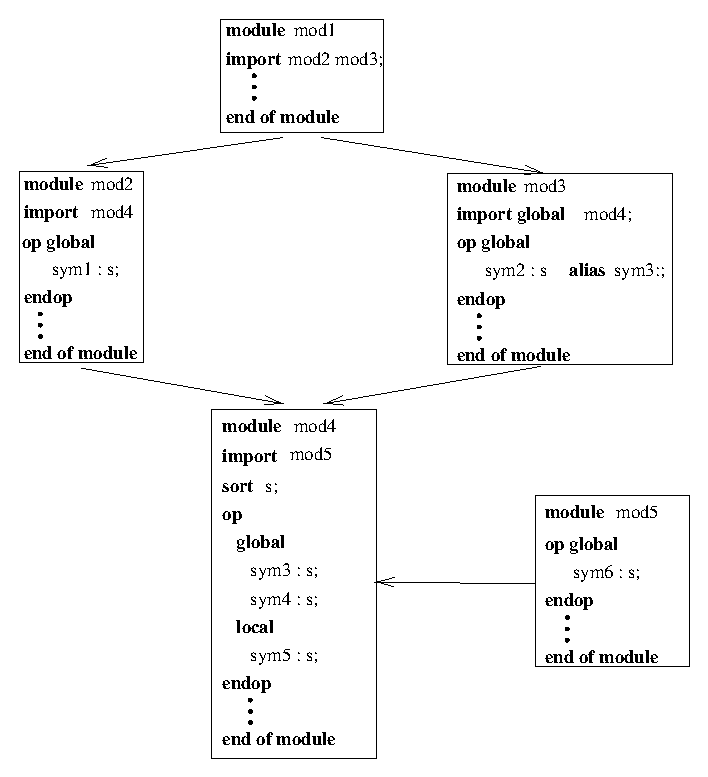
\psfig{figure=im_elan1.eps}
%%\end{minipage} \end{center}
%%In this situation:
%%\begin{itemize}
%%\item The sort {\tt s} is visible in all modules,
%%\item {\tt sym5} is visible only in {\tt mod4},
%%\item {\tt sym4} is visible in modules {\tt mod1}, {\tt mod2}, {\tt mod3}, and {\tt mod4},
%%\item {\tt sym3} is visible in the modules {\tt mod2}, {\tt mod3} and {\tt mod4} and it is
%%       also visible in {\tt mod1} but under the name {\tt sym2},
%%\item {\tt sym2} is just another name for {\tt sym3} and it is only visible in
%%        module {\tt mod1} and {\tt mod3},
%%\item {\tt sym1} is only visible in modules {\tt mod1} and {\tt mod2}.
%%\end{itemize}
%%\FEX
%%04-12-98 : l'exemple est dans l'ancienne syntaxe.

\subsection{Built-in modules}

For convenience and efficiency several modules are provided as
built-ins. See section~\ref{les built-in} for a full description of
the current available ones.

% the following modules are built-in
% \elan:
% \begin{enumerate}
%   \item {\tt anyInteger} provides the sort {\tt int} and all 
%           constants 0, 1, -1, 2, \ldots. A description of this module
%           is given in the standard library, see
%           page~\pageref{anyInteger module}.
%   \item {\tt anyIdentifier} provides the sort {\tt ident} and all 
%           constants a, b, c, aa, ab, \ldots. A description of this module
%           is given in the standard library, see
%           page~\pageref{anyIdentifier module}.
%   \item {\tt anyQuotedIdentifier} provides all quoted
%           constants ``a'', ``b'', ``c'', ``aa'', ``ab'', \ldots. A description
%           of this module is given in the standard library, see
%           page~\pageref{anyQuotedIdentifier module}.
% \end{enumerate}
% These modules can be imported as standard ones.

\subsection{Parameterised modules}

Parameterised modules can be defined in \elan\ as follows:

\grrule{formal module name}{
  \nt{identifier}
\gror
  \nt{identifier} \sym{[} \nt{identifier} \itzero{\sym{,}\nt{identifier}}
                  \sym{]}
}

The module instantiation by its actual parameters is currently done by
the syntactical replacement of the formal arguments by the actual ones.

\EX The classical example is the one of parameterised lists:\\
\insertExamples{simpleList.eln}

\noindent
and we get list of integers by 
instantiating {\tt X} by {\tt int} and importing {\tt int} as in:\\
\insertExamples{simpleList.lgi}
\FEX

%\EX [ck: Oct 29 97] exemple deja donne avant!
%Another classical example is based on the parameterised programming
%paradigm as advocated in~\cite{Goguen-HOF-unnecessary-90}:\\
%\insertExamples{map.eln}
%
%\FEX


\subsection{LGI modules}
\label{subsec.lgi.module}

The top level description of the logic consists of:
\begin{enumerate}
\item the description of the syntax that the user is allowed to use in
        order to give his specifications.
\item the description of a term, called the query, that will be reduced
        in the rewrite logic defined by the (super) user.
\end{enumerate}

The syntax is the following:
\grrule{lpl description}{
\rw{LPL} \nt{identifier} \rw{description}    \nl
\omm{\nt{specification description}}                  \nlp{5}
\rw{query}                                      \nlp{15}
        \rw{of sort} \nt{sort name}               \nlp{15}
        \rw{result of sort} \nt{sort name}       \nlp{15}
        \rw{import} \itone{\nt{instantiated module name}} \nlp{15}
        \omm{\rw{check with} \nt{boolean term}}         \nlp{15}
        \rw{start with} \nt{start term}          \nl
\rw{end}
}

\grrule{specification description}{
\rw{specification description}                  \nl
  \itone{\nt{specification part description}}   \nl
\rw{end}                                        
}

\grrule{specification part description}{
\rw{part} \nt{identifier}                 \nlp{10}
\rw{of sort} \nt{sort name}        \nlp{10}
\rw{import} \itone{\nt{instantiated module name}}        \nlp{10}
\omm{\rw{check with} \nt{boolean term}}   
}

\grrule{start term}{\sym{(} \omm{\nt{Estrategy name}} \sym{)} \nt{query term}}

The syntax of of \nt{query term} is built over the user-defined
signature enriched by the constant {\bf query}. The sort of {\bf
query} is given by the query declaration above.

\EX If no specification is needed, the specification description part
is skipped, as in the 
following logic description used for running
Example~\ref{testStrat.eln}:\\

\insertExamples{testStrat.lgi}
\FEX

\EX \label{unif.lgi.example}
Here is a simple example of the top level description of how unification can 
be implemented:\\
\insertExamples{unification.lgi}
\noindent
In this unification logic, the user should provide the specification
information as follows:\\
\insertExamples{simplesig.spc}

The user should use the (super-user defined) keywords {\tt Vars} and
{\tt Ops} to define respectively the variables and the operators,
namely {\tt a} of arity 0, {\tt f} of arity 2, etc...

\FEX

\subsubsection{Semantics}

When parsing a specification, \elan\ generates new modules that
 complete the definition of the rewrite theory to be used during the
 evaluation of the query. For instance, in the case of the previous
 example, these new modules are:
\\
\insertExamples{moduleVarUnif.eln}

\noindent
and\\
\insertExamples{moduleOpsUnif.eln}

When a user provides a specification to an \elan\ logic, this simply
provides more information about the context in which the user wants
to work, like the name of function symbols or basic axioms to use.

\section{Pre-processing}
\label{preprocessor}

Another original feature proposed by \elan\ is the use of a
pre-processing phase that allows to describe the logic to be encoded
in an easier way.

As described in Figure~\ref{elan-principle}, the pre-processor is
performing textual replacements starting from informations given by
the super-user in the modules, and by the user in the specification
file. The pre-processing phase in \elan\ can just be thought of as a
macro expansion mechanism which extends the parameterization process
described before.

In order to express the syntax of the pre-processor construction, we
need the notion of {\it constant expression} and of {\it text} defined
as follows:

\grrule{constant expression} {
        \nt{number}
\gror
        \sym{(}\nt{subexpression}\sym{)}
}

\grrule{subexpression} {
        \nt{number}
\gror
        \nt{subexpression} \sym{+} \nt{subexpression}
\gror
        \nt{subexpression} \sym{-} \nt{subexpression}
\gror
        \nt{subexpression} \sym{*} \nt{subexpression}
\gror
        \nt{subexpression} \sym{/} \nt{subexpression}
\gror
        \nt{subexpression} \sym{\%} \nt{subexpression}
\gror
        \sym{(}\nt{subexpression}\sym{)}
}

\grrule{lexem}{
      \nt{identifier}
\gror \nt{number}
\gror \nt{char}
}

\grrule{text}{\itone{\nt{lexem}}}

\subsection{Simple duplication}

A first feature is to allow simple duplications of a part of text. The
syntax is:

\grrule{simple repetition} {
  \nt{lexem}\symmm{$\tilde{\ }$}\nt{constant expression}
\gror
  \sym{\{} \nt{text} \sym{\}}\symmm{$\tilde{\ }$}\nt{constant expression}
}

\EX
The text ``$\tt a\{, b\}\tilde{\ }3$'' is processed into ``{\tt a, b,
b, b}''. 
\FEX

\subsection{Duplication with argument}

It is often necessary to allow description of objects like
$f(t_1,\ldots,t_5)$. This is possible using the syntax:


\grrule{arg.repetition}{
  \sym{\{} \nt{text} \sym{\}}\symmm{\_}
  \nt{identifier} \nl
  \sym= \nl
  \nt{constant expression} \sym{...} \nt{constant expression}}

\EX
The text ``{\tt P \{ \& s\_I=t\_I \}\_I=1...3}'' is processed into
``{\tt P  \& s\_1=t\_1 \& s\_2=t\_2  \& s\_3=t\_3}''. 
\FEX

A special form of this duplication with arguments is the explicit
construction of a list of indexed identifiers allowed using the
syntax:

\grrule{arg.repetition}{
  \nt{identifier}\symmm\_\nt{number}\nt{char}\sym{...}\nt{char}
  \nt{identifier}\symmm\_\nt{number}
}

\EX
The text ``{\tt t\_1,...,t\_5}'' is processed into ``{\tt t\_1 , t\_2
, t\_3 , t\_4 , t\_5}''. 
\FEX

\subsection{Enumeration using FOR EACH}\label{for each}

This construction allows to make the link between the specification
given by the user and the logic described by the super-user. A natural
motivation for this construction is given by the ``standard'' way
inference rules are used. For example when describing how unification
works, the following transformation rule is given:
\renewcommand{\fleche}{\ra}
\uneregle{Decompose}
        {P \ww \f{s}{n} \eqq \f{t}{n} }
        {P \ww s_1 \eqq t_1\ww \ldots \ww s_n \eqq t_n }
It is generic in the sense that the operator $f$ is unspecified. It
can be a $+$ of arity 2, or a $if@then@else@$ of arity 3, or just a
constant. We do not want, when specifying how the logic works, to give
only the specific cases, we need to be as generic as possible.

\elan\ provides via the FOR EACH construction of the pre-processor, a
way to be generic. The syntax is the following:

\grrule{for each const.} {
  \rw{FOR EACH} \nt{vardecl} \rw{SUCH THAT} \nt{varaffect} \sym{: \{}\nlp{5}
     \nt{text} \nl
  \sym{\}}
}

\grrule{vardecl}{
  \nt{varname}\itzero{\sym,\nt{varname}} \sym: \nt{sort name}
\gror
  \nt{vardecl}\sym;\nt{vardecl}
}

\grrule{varaffect}{
  \nt{varname} \sym{:= (} \omm{\nt{strategy name}} \sym) \nt{term}
\gror
  \nt{varaffect} \rw{AND} \nt{varaffect}
\gror
  \nt{varaffect} \rw{ANDIF} \nt{boolean term}
}

\Attention{
Since the symbols {\tt \{, \},$ \tilde{\ }$} are reserved for
pre-processor use, it is not possible to use them for any other
purpose, even quoted.
}

\Attention{
The pre-processor uses the character `\_' (underline) for assembling
identifiers. For example, the text `{\tt a f \_1\_ x b}'' is pre-processed
into the sequence of three identifiers {\tt a}, {\tt f\_1\_x} and {\tt
b}. The character `\_' is thus part of an identifier even if there is
a space between it and the rest of the string. It is thus better for
the user not to use the \_ symbol, except for building identifiers of course.
}

\EX
The rule \rname{Decompose} that we mentioned at the beginning of
this section can be expressed in the following way:\\
\insertExamples{decomposition.eln}

If the specification given by the user consists in the operator symbols
{\tt f} and {\tt g} of respective arities 2 and 1, then the
pre-processor expands the previous {\bf FOR EACH} construction into:\\
\insertExamples{decompositionExpanded.eln}

\FEX


\section{Differences with previous version of the language}
\label{versionChanges}

The language has evolved a lot between \elan\ version 1.17 and \elan\
version 3.0. The changes concern the syntax of:
\begin{itemize}
  \item modules,
  \item rules and
  \item strategies.
\end{itemize}

The main changes are emphasized in the corresponding sections of the
language description, and the main concern has been to uniformize the
language constructions.

The transformations needed to change from the syntax of version 1.17 to the
current one (i.e. later than 2.00) are summarized below.

Concerning the declaration parts:
\begin{itemize}
\item \texttt{import ...} becomes \texttt{import ... end}
\item \texttt{sort ...} becomes \texttt{sort ... end}
\item \texttt{op ... endop} becomes \texttt{operators ... end}
\end{itemize}
Now, there is only one construction to define rules, you have to
replace: 
\begin{itemize}
\item \texttt{rule for ...} by \texttt{rules for ...}
\item \texttt{rule <name> for ...} by \texttt{rules for ... [name] ...}
\item suppress \texttt{declare} keyword
\item \texttt{body} or \texttt{bodies} by \texttt{global} or
  \texttt{local}
\item \texttt{end of rule}, \texttt{end of rules} by \texttt{end}
\end{itemize}

The rule labels accept now arguments that should be variables involved
in the rule.

Definition of strategies looks like rules definitions, you have to
replace: 
\begin{itemize}
\item \texttt{strategy ...} by \texttt{strategies for ... global|local
    [name] ...} 
\item \texttt{iterate ... enditerate} by \texttt{iterate*(...)}
\item \texttt{while ... endwhile} by \texttt{repeat*(...)}
\item \texttt{repeat ... endrepeat} by \texttt{repeat*(...)}
\item \texttt{dont know choose(...)} by \texttt{dk(...)}
\item \texttt{dont care choose(...)} by \texttt{dc(...)}
\item \texttt{end of strategy} by \texttt{end}
\item \texttt{end of module} by \texttt{end}
\end{itemize}
Local affectations and conditions are now evaluated from top to
bottom. The order of presentation has been reversed, so that the {\em
old} syntax:
\begin{verbatim}
  [] l => r
          if c2
          where v2:=(...) ...
          where v1:=(...) ...
          if c1
\end{verbatim}
becomes in the {\em new} syntax:
\begin{verbatim}
  [] l => r
          if c1
          where v1:=(...) ...
          where v2:=(...) ...
          if c2
\end{verbatim}



\chapter{\elan: the system}
% Document Type: LaTeX
% Master File: manual.tex

%%%% \chapter{\elan: the system}

This section is devoted to the user environment of the \elan{}\
language, and is partly borrowed from~\cite{BorovanskyKKMR-WRLA98}.

%%%%%%%%%%%%%%%%%%%%%%%%%%%%%%%%%%%%%%%%%%%%%%%%%%%%%%%%%%%%
\section{Global architecture}
%%%%%%%%%%%%%%%%%%%%%%%%%%%%%%%%%%%%%%%%%%%%%%%%%%%%%%%%%%%%

The \elan\ environment consists of several components, as depicted in
Figure~\ref{ELAN-env}. The preprocessor expands a few concise
constructions allowed  in the language.
The parser checks the syntax of programs and verifies that terms are
syntactically well-formed.  The interpreter is an interactive tool
allowing the user to check that the results he expects are indeed
obtained. Initially, the preprocessor and the parser were integrated
in the interpreter and so it was not possible to call them as
stand-alone processes.  The compiler transforms specifications into
independent executable \texttt{C} code (Section~\ref{compilo}). It is
a stand-alone tool without any preprocessing and parsing
facilities. The preprocessing and parsing phases are provided by the
interpreter, which communicates the result of these processes to the
compiler via a data exchange format called \REF. Section~\ref{ref_format}
describes some tools to translate \elan\ to \REF\ and vice versa.
Especially, the translation from \elan\ to \REF\ performed by the 
\texttt{query2ref} tool relies mainly on reusing the parser initially
integrated in the interpreter.

\begin{figure*}[ht] %zoom 50
\centering
\input{ELAN-env.pstex_t}
\label{ELAN-env}
\caption{Global architecture of the \elan\ environment}
\end{figure*}


%%%%%%%%%%%%%%%%%%%%%%%%%%%%%%%%%%%%%%%%%%%%%%%%%%%%%%%%%%%%
\section{The preprocessor}
%%%%%%%%%%%%%%%%%%%%%%%%%%%%%%%%%%%%%%%%%%%%%%%%%%%%%%%%%%%%

The \elan\ syntax provides a few fancy constructions to perform
textual replacements. So the preprocessor may be used to automatically
generate parts of specifications used to analyse the rest of a
program.  It should be emphasised that there is strong interaction
between the parser, the preprocessor and the interpreter. 
See Section~\ref{preprocessor} for a description of the preprocessor
functionality. 


%%%%%%%%%%%%%%%%%%%%%%%%%%%%%%%%%%%%%%%%%%%%%%%%%%%%%%%%%%%%
\section{The parser}
%%%%%%%%%%%%%%%%%%%%%%%%%%%%%%%%%%%%%%%%%%%%%%%%%%%%%%%%%%%%

The \elan\ parser is based on Earley's one~\cite{Earley} and is using sort
informations in order to determine as soon as possible in the analysis
the right choice. This explains why in the current version, some
construction of the language
require to give the sort information together with the term.

%%%%%%%%%%%%%%%%%%%%%%%%%%%%%%%%%%%%%%%%%%%%%%%%%%%%%%%%%%%%
\section{The interpreter}
%%%%%%%%%%%%%%%%%%%%%%%%%%%%%%%%%%%%%%%%%%%%%%%%%%%%%%%%%%%%


The interpreter takes a well-formed program and a well-formed query
(both checked by the parser) and applies the rules and strategies
defined in the program to the query. In order to find which rules can
apply, the selection is guided by the top symbol of the rules: only
those rules whose left-hand side has the same top symbol as the term
to be reduced are selected. They are then tried in the order given in
the program.  Another kind of choices arbitrarily made by the
interpreter is for the strategy $\dc(S_1,...,S_n)$ that should select
randomly a non-failing strategy among $S_1,...,S_n$. In practice, the
interpreter selects the first one, so implements \dc\ and \first\ in the
same way. Note however that there exists a  version of
\elan\ which concurrently executes the $n$ strategies and selects the
first one which terminates without failure~\cite{BorovanskyCastro-WRLA98}.

Once a set of rules is selected, a many-to-one matching algorithm 
is applied. When associative and
commutative  ($AC$ for short) operators are involved, an external 
one-to-one $AC$-matching algorithm described in~\cite{Eker-AcMatch-95}
is called. 
This algorithm is not fully integrated in the interpreter, so 
data structure conversions are required and lower the efficiency of
the $AC$-matching, already  quite complex.
Once a match is found, local evaluations are performed and if all 
succeed, the result term is built, taking advantage of the right-hand 
side of the rule and of term sharing.


%%%%%%%%%%%%%%%%%%%%%%%%%%%%%%%%%%%%%%%%%%%%%%%%%%%%%%%%%%%%
\section{The compiler}
\label{compilo}
%%%%%%%%%%%%%%%%%%%%%%%%%%%%%%%%%%%%%%%%%%%%%%%%%%%%%%%%%%%%

The \elan{} compiler transforms a logic description into an executable
binary file.  The compiler (for detailed description,
see~\cite{Vittek-RTA96,MoreauK-PLILP+ALP98}) produces an efficient
\verb|C| code, which is later compiled by the \verb|cc| or the
\verb|gnu gcc| compiler. 
The executable binary code is dependent on the particular
architecture, because a small part of the \elan{} library performing
the basic non-deterministic operations is written in assembly
language~\cite{Moreau-JICSLPW98}.
Up to now, this is the only reason that makes
the compiler available only on the architectures DEC-ALPHA, SUN4 and
Intel-PC.  
%This release of the \elan{} compiler does not compile the
%whole \elan{} language: the main restriction is that the \elan{}
%compiler does not treat Input/Output and reflective capabilities of
%the interpreter. There is also a restriction on the class of rules
%containing AC-symbols that can be compiled.

\subsection{Non-linear rules}
%%%%%%%%%%%%%%%%%%%%%%%%%%%%%%%%%%%%%%%%%%%%%%%%%%%%%%%%%%%%
The \elan\ compiler does not support non-left-linear rules (a rule is
called non-left-linear if a variable occurs more than once in the
left-hand side).
The many-to-one matching algorithm only compiles linear rules. 
The \elan\ parser automatically transforms non-left-linear rules into
left-linear conditional rules by renaming variables that occurs more
than once and adding some conditions to ensure their equality.

For example, the rule \texttt{f(x,x) => g(x)} is transformed into
\texttt{f(x,y) => g(x) if x==y}.


\subsection{Built-ins}
%%%%%%%%%%%%%%%%%%%%%%%%%%%%%%%%%%%%%%%%%%%%%%%%%%%%%%%%%%%%
To be more efficient, builtin data type such as
\textit{builtinInt} and \textit{identifier} are compiled in a
particular way. 

The main drawback of this approach is that only completely defined
functions can be defined on builtin data type.

Let \texttt{f(@) : (builtinInt) builtinInt} be an operator. 
For each integer $n$, $f(n)$ must be reducible to an integer. Suppose
defined the rule 
\texttt{[] f(n) => n-1 if n > 1}, the term \texttt{f(0)} can not be
reduced to a builtin integer. In this case, behaviour is undefined.
This explains why \textit{builtinInt} are never used directly: it is
recommended to use the sort \textit{int} which is no longer a builtin
data type.


\subsection{Input/Output facilities}
\label{IO switches}
%%%%%%%%%%%%%%%%%%%%%%%%%%%%%%%%%%%%%%%%%%%%%%%%%%%%%%%%%%%%
Input/Output facilities are now fully  implemented in the compiler. 
Their syntax is described in the module {\bf IO.eln} of the standard library. 

As in the version V3.4, it is possible, in the generated 
program, to enter a query term in the \elan\ syntax, just like in the
interpreter. In the same way, result terms computed by the generated
program are now pretty-printed in the \elan\ syntax. Therefore, it is
no more necessary to give a fixed ground term in the \verb|.lgi| file, 
and \verb|.lgi| files involving the \verb|query| keyword can now be
compiled. In the current version, the query is parsed dynamically in 
the generated program by reusing a subpart of the parser integrated to
the interpreter. 

The generated program can be executed with several switches used to
specify the different possible formats of input (query) and output
(result) terms:

\paragraph{Input switches}

\begin{itemize}

\item \verb|-REFInput|: the query term must be in the \REF\ 
  format (see Section~\ref{ref_format}). 

\item \verb|-noInput|: the query ground term is supposed to 
  be located in the \verb|.lgi| file, where it replaces the
  \verb|query| keyword. 


\end{itemize}



\paragraph{Output switches}

\begin{itemize}

\item \verb|-REFOutput|: result terms will be given in the
  \REF\ format (see Section~\ref{ref_format}). 

\item \verb|-noOutput|: results are computed but not
  written out. The interest of this switch is rather limited, but it
  can be useful for people who only want the statistics of the
  computation, like the number of rewrite steps per seconds. 

\item \verb|-internalOutput|: result terms are given by using a prefix 
  notation. This is the original syntax used in the first version of
  the compiler. 

\end{itemize}

The generated program, called by default \textit{a.out}, can 
be executed with some other switches not necessarily related to
Input/Ouput, like \verb|a.out -quiet| or \verb|a.out -debug|.


At this point, it is still possible to change the content of the
\verb|start with| instruction declared in the \verb|.lgi| file. The switch
\verb|-strategy|~\nt{strategy name}~{\bf :}~\nt{sort name} will apply the
strategy \nt{strategy name} on a query term of sort \nt{sort
  name}. 


Similarly, the switch \verb|-sort|~\nt{sort name} will apply 
the empty strategy on a query term \nt{sort name}. Note that
\verb|-strategy| and \verb|-sort| are mutually exclusive. 

\Attention{
The list of available sorts (resp. strategy names) can be found in the
\texttt{.ref} file.
} 


%%%%%%%%%%%%%%%%%%%%%%%%%%%%%%%%%%%%%%%%%%%%%%%%%%%%%%%%%%%%
\section{The \REF\ format}
%%%%%%%%%%%%%%%%%%%%%%%%%%%%%%%%%%%%%%%%%%%%%%%%%%%%%%%%%%%%
\label{ref_format}


The Reduced \elan\ Format, \REF\ for short, is a term-like
representation of \elan\ programs introduced both for the
interconnection of software components involved in the \elan\ system,
and for combining \elan\ programs. This format is also of greatest
interest for the implementation of reflection techniques in \elan. 
A detailed description of its applications can be found
in~\cite{BorovanskyKKMR-WRLA98}. 

The \REF\ format has been initially developed to reuse the powerful
Earley's parser integrated in the interpreter. By loading with the
interpreter an \elan\ program possibly in mixfix notation, we can get a
\REF\ program which can be viewed as the external representation of
the interpreter working memory. \REF\ is easier to parse than \elan\
since the \REF\ grammar is simply LALR.  
The \elan\ interpreter generates a \REF\ file
\textit{prog.ref} thanks to the option \texttt{--export}:
\begin{verbatim}
elan --export prog.ref prog.lgi [prog.spc]
\end{verbatim}
The \REF\ program contained in \textit{prog.ref} can be directly
executed by the interpreter as follows:
\begin{verbatim}
elan --import prog.ref
\end{verbatim}
Then, the behavior of the interpreter is exactly the one expected
with the command:
\begin{verbatim}
elan prog.lgi [prog.spc]
\end{verbatim}
but without the time-consuming preprocessing and parsing phases.

The core of the \elan\ compiler, called REM for ``Reduced \elan\ Machine'' and
implemented in \texttt{Java}, only knows the \REF\ syntax. This
explains why we need a script \texttt{elanc} to first call the
interpreter in order to obtain a \REF\ file, and second to execute REM
with this \REF\ file as input. 

Then, a compiled \texttt{C} program, 
say \texttt{a.out}, is generated by REM. This program can be executed
with different options like \texttt{a.out -REFInput}, \texttt{a.out -REFOutput}
or even better \texttt{a.out -REFInput -REFOutput}:
\begin{itemize}
\item The option \texttt{-REFInput} reads a new query in \REF\ syntax to replace
the ground query occurring initially in \textit{prog.lgi}.
\item The option \texttt{-REFOutput} writes all result terms computed by
\textit{a.out} in \REF\ syntax, instead of the \elan\ syntax used by
default. 
\end{itemize}

So, we still have to convert an \elan\ 
query to a \REF\ query, and conversely to retrieve the \elan\ syntax
of result terms written in \REF\ syntax. 

For this purpose, one can use another
tool to read a query and to pretty-print result terms of the \textit{a.out}
program, both in \elan\ syntax, similarly to the interpreter.
This tool is called \texttt{prettyIO} and may be used as follows:
\begin{verbatim}
prettyIO a.out prog.ref
\end{verbatim}
Note that \textit{prog.ref} is needed to find the \elan\ syntax of
functions implemented by \textit{a.out}, and so to encode a query
term provided by the user in \elan\ syntax, and to decode terms
written in \REF\ syntax by \texttt{a.out -REFInput -REFOutput}. 
The executable \texttt{prettyIO} is implemented as a script calling
some basic tools:  

\begin{itemize}

\item \texttt{query2ref prog.ref} reads repeatedly (from
\texttt{stdin}) a sort, and parses a term of this sort written in 
\elan\ syntax. The result (written to \texttt{stdout}) 
is the corresponding term in \REF\ syntax.
By using the option \texttt{--query} as follows: 
\begin{verbatim}
query2ref prog.ref --query
\end{verbatim}
we only parse terms of the sort of the query, as indicated in
\textit{prog.lgi} (this information also occurs in \textit{prog.ref}).

\item \texttt{ref2result prog.ref} reads repeatedly (from \texttt{stdin})
terms encoded  in \REF\ syntax and writes (to \texttt{stdout}) 
the related terms in \elan\ syntax, by using the signature 
occurring in \textit{prog.ref}.

\end{itemize}

The script \texttt{prettyIO} is located in the directory \texttt{bin/}
like \texttt{elanc}, and the compiled \texttt{C/C++} programs
\texttt{query2ref} and \texttt{ref2result} are located in the
subdirectory of \texttt{bin/} related to the current system
architecture, like the interpreter \texttt{elan}.


\Attention{
The user should be aware that \texttt{prettyIO} is much 
less interesting in the current version, since it is now possible to
parse a query term and to pretty-print all results by simply using the
generated program \textit{a.out} itself. 
}


%%% Local Variables: 
%%% mode: latex
%%% TeX-master: t
%%% TeX-master: t
%%% End: 


\chapter{The standard library and the built-ins}\label{library}
% -*- Document-Type: LaTeX; Master-File: manual.tex -*- 

% [ck: Aug  9 95]
% \chapter{The standard library}


This chapter presents the main features of the \elan\ standard
library. Remember that the path to this library is specified in the system variable ELANLIB whose default value is set to the subdirectory {\tt elan\_library/elanlib} of the source directory. \elan\ can be used without any reference
to this library, {\it except\/} for what concerns the use of the
built-in objects which are documented in the second part of this chapter.

This   library has  been   designed to  be small  and  as efficient as
possible.   In  particular  {\it  no\/}  AC   operators  is used.  The
resulting  code is more  efficient, at  the  price of sometimes heavier
descriptions.


\section{The \elan\ standard library}

The standard library is fully documented in~\cite{elanlibManual-98} to 
which we refer for details. We give below the list of files defined in
the standard library. Some of them define built-in sorts and operators
and in this case, they also appear in the next section 
(section~\ref{les built-in}).

\subsection{common}

In this category, the most common abstract data types are defined.


\begin{tabular}{l@{~~~~~}l}
        anyIdentifier.eln            &  eq.eln\\
        anyInteger.eln               &  identity.eln\\
        array.eln                    &  int.eln\\
        arrayLIN.eln                 &  integerConstants.eln\\
        arrayLOG.eln                 &  IO.eln\\
        bool.eln                     &  list.eln\\
        builtinArray                 &  occur.eln\\
        builtinHashTree              &  pair.eln\\
        builtinInt.eln               &  prompt.eln\\
        builtinIO.eln                &  replace.eln\\
        builtinSidio.eln             &  stdio.eln\\
        builtinString.eln            &  string.eln\\
        builtinSyntacticMatching.eln &  strlist.eln\\
        cmp.eln                   &  tuple.eln\\
        Query.eln\\
\end{tabular}

\subsection{ref}

All the modules needed to deal with the Reduced \elan\ Format.

\begin{tabular}{l@{~~~~~}l}
        Meta\_Apply.eln         ref\_modules.eln        ref\_terms.eln \\
        REF.eln                ref\_read.eln           ref\_unify.eln \\
        ref\_rules.eln          ref\_unify\_builtin.eln \\
        ref2string.eln         ref\_sorts.eln          ref\_write.eln \\
        ref2term.eln           ref\_strategies.eln     refstring2string.eln \\
        ref\_idents.eln         ref\_tables.eln         string2refterm.eln
\end{tabular}

\subsection{noquote}

These modules describe a possible syntax for the user
specifications. More complicated syntax (e.g. mixfix) can also be
defined.

\begin{tabular}{l@{~~~~~}l}
        applySubstOn.eln   hornClauseSyntax.eln    syntacticUnification.eln \\
        atom.eln           ident.eln               termCommons.eln \\
        atomP.eln          identifier.eln          sigSyntax.eln \\
        eqSystem.eln       substitution.eln
\end{tabular}

\subsection{strategy}

These modules are used for the definition and evaluation of defined
strategies.

\begin{tabular}{l@{~~~~~}l}
        Any.eln          booleg.eln       meta.eln         strsig.eln \\
        any.eln        Meta\_apply.eln   strapply.eln     symbol.eln \\
        Meta\_capply.eln  commit.eln       strat.eln        tcstrat.eln \\
        Meta\_strat.eln   strcapply.eln   loops.eln        strconc.eln
\end{tabular}

\section{The built-ins}\label{les built-in}

%\section{The built-ins}\label{les built-in}
%%% General comment 

There are two types of built-in symbols:
\begin{itemize}
\item 
  {\bf The built-in constructors}, which are non-reducible
  symbols, built into the \elan\ system. Terms built over them are
  either constructed, or interpreted by the \elan\ system, e.g. the
  symbol {\tt Error} defined in the module
  {\ldots/common/builtinIO.eln} as follows:\\
    \begin{verbatim}
    Error(@) : (builtinInt) X   code 122;
    \end{verbatim}
    which is used to report various errors of the I/O sub-system
    written in C++.
\item
    {\bf The built-in functions}, which represent symbols with
    pre-defined semantics, in general, not [easily] specifiable in
    \elan\ itself.  The symbol {\tt open} in  the module
    {\ldots/common/builtinStdio.eln} defined as follows:\\
  \begin{verbatim}
   open_builtinStdio(@,@)     : (builtinString builtinString) builtinInt code 116;
  \end{verbatim}
    can be taken as an example.  In this case, the declaration
    (profile) of the symbol {\tt open} represents an interface between
    the \elan\ specification and its built-in semantics. In this case,
    the code ``116'' identifies its semantics.
    
    If there is an overloaded built-in symbol whose exact semantics
    depends on its profile, a procedure implementing the built-in
    symbol should know, which instance of the built-in symbol is
    executed. The overloaded symbol
    {\tt read\_builtinIO} is an example of this problem:\\
  \begin{verbatim}
    read_builtinIO(@,@)      : (builtinInt X) X   pri 200 code 120;
  \end{verbatim}
    When the built-in symbol {\tt read\_builtinIO} is used for several sorts {\tt
      X}, there exist several built-in symbols {\tt read\_builtinIO} in the
    user's specification.  All of them are linked with the same
    semantic function (with the code 120) parameterized by the
    concrete profile of {\tt read\_builtinIO}. Thus, the sort of a read term is
    known in the semantic procedure due to the profile of actually
    applied symbol {\tt read\_builtinIO}.  The difference between two kinds of
    {\em built-in function} symbols is expressed by the sign of code
    numbers.
\end{itemize}


\subsection{Booleans}

At the beginning there is nothing, so \elan\ provides the true and
false values and introduces the bool module. These two values are
built-in and are deeply connected to the implementation of conditions
in rewrite rules. 

\subsubsection{/elanlib/common/bool.eln}

%% Hubert 

\begin{tabular}{|c|c|c|p{8cm}|}
\hline
{\bf Builtins} & {\bf Code} & {\bf Signature} & {\bf Comments} \\
\hline
\hline
{\tt false}     & 0 & {\tt () bool} & The logical {\tt false}.\\
{\tt true}      & 1 & {\tt () bool} & The logical {\tt true}.\\
{\tt @ and @}   & 21 & {\tt (bool bool) bool} & The logical conjonction.\\
{\tt @ or @}    & 22 & {\tt (bool bool) bool} & The logical disjonction.\\
{\tt not(@)}    & 24 & {\tt (bool) bool} & The logical negation.\\
{\tt @ == @}    & 8 & {\tt (bool bool) bool} & The logical equality test.\\
{\tt @ != @}    & 9 & {\tt (bool bool) bool} & The logical inequality test.\\
{\tt @ $<$ @}   & 10 & {\tt (bool bool) bool} & A logical test assuming that {\tt false<true}.\\
{\tt @ $<$= @}  & 11 & {\tt (bool bool) bool} & A logical test assuming that {\tt false<true}.\\
{\tt @ $>$ @}   & 12 & {\tt (bool bool) bool} & A logical test assuming that {\tt false<true}.\\
{\tt @ $>$= @}  & 13 & {\tt (bool bool) bool} & A logical test assuming that {\tt false<true}.\\
\hline
\end{tabular}


\subsubsection{/elanlib/common/cmp.eln}

%% Hubert

To enrich the booleans, {\it polymorphic\/} equality, disequality and
inequalities are defined and are also built-in:\\

\noindent \begin{tabular}{|c|c|c|p{9cm}|}
\hline
{\bf Builtins} & {\bf Code} & {\bf Signature} & {\bf Comments} \\
\hline
\hline
@ == @          & 18 & {\tt (X X) bool} & Tests the equality between two elements of the same sort {\tt X}.\\
@ != @          & 19 & {\tt (X X) bool} & Tests the inequality between two elements of the same sort {\tt X}.\\
%% @ $<$ @      & 30 & {\tt (X X) bool} & \\
%% @ $<$= @     & 31 & {\tt (X X) bool} & \\
%% @ $>$ @      & 32 & {\tt (X X) bool} & \\
%% @ $>$= @     & 33 & {\tt (X X) bool} & \\
\hline
\end{tabular}



\subsection{Numbers}

Numbers can of course be created ``by hand'', but we choose in \elan\
to provide built-in integers.\\

\subsubsection{/elanlib/common/builtinInt.eln}

%% Hubert

\begin{tabular}{|p{3cm}|c|c|p{4cm}|}
\hline
{\bf Builtins} & {\bf Code} & {\bf Signature} & {\bf Comments} \\
\hline
\hline
{\tt @ + @}                             & 3 & {\tt (builtinInt builtinInt) builtinInt} & The addition on integers.\\
{\tt @ - @}                             & 4 & {\tt (builtinInt builtinInt) builtinInt} & The soustration on integers.\\
{\tt @ * @}                             & 5 & {\tt (builtinInt builtinInt) builtinInt} & The multiplication on integers.\\
{\tt @ / @}                             & 6 & {\tt (builtinInt builtinInt) builtinInt} & The division on integers.\\
{\tt @ \% @}                            & 27 & {\tt (builtinInt builtinInt) builtinInt} & The modulo operation.\\
{\tt @ \& @}                            & 28 & {\tt (builtinInt builtinInt) builtinInt} & {\tt a \& b} makes the logical conjonction between the binary representations of {\tt a} and {\tt b} and returns the corresponding integer.\\
{\tt @ $|$ @}                           & 29 & {\tt (builtinInt builtinInt) builtinInt} & {\tt a $|$ b} makes the logical disjonction between the binary representations of {\tt a} and {\tt b} and returns the corresponding integer.\\
{\tt - @}                               & 20 & {\tt (builtinInt) builtinInt} & The opposite of any integer.\\
{\tt @ == @}                            & 8 & {\tt (builtinInt builtinInt) bool} & The equality test.\\
{\tt @ != @}                            & 9 & {\tt (builtinInt builtinInt) bool} & The inequality test.\\
{\tt @ $<$ @}                           & 10 & {\tt (builtinInt builtinInt) bool} & The strict ordering test between integers.\\
{\tt @ $<$= @}                          & 11 & {\tt (builtinInt builtinInt) bool} & The ordering test between integers.\\
{\tt @ $>$ @}                           & 12 & {\tt (builtinInt builtinInt) bool} & The strict ordering test between integers.\\
{\tt @ $>$= @}                          & 13 & {\tt (builtinInt builtinInt) bool} & The ordering test between integers.\\
{\tt eq\_builtin Int(@,@)}              & 8 & {\tt (builtinInt builtinInt) bool} & The equality test.\\
{\tt neq\_builtin Int(@,@)}             & 9 & {\tt (builtinInt builtinInt) bool} & The inequality test.\\
{\tt less\_builtin Int(@,@)}            & 10 & {\tt (builtinInt builtinInt) bool} & The strict ordering test between integers.\\
{\tt lesseq\_builtin Int(@,@)}          & 11 & {\tt (builtinInt builtinInt) bool} & The ordering test between integers.\\
\hline
\end{tabular}
~\\
\begin{tabular}{|p{3cm}|c|c|p{5,5cm}|}
\hline
{\bf Builtins} & {\bf Code} & {\bf Signature} & {\bf Comments} \\
\hline
\hline
{\tt greater\_builtin Int(@,@)}         & 12 & {\tt (builtinInt builtinInt) bool} & The ordering test between integers.\\
{\tt greatereq\_ builtinInt(@,@)}       & 13 & {\tt (builtinInt builtinInt) bool} & The ordering test between integers.\\
{\tt btoi(@)}                           & 25 & {\tt (bool) builtinInt} & The conversion from a boolean to an integer ($false$ becomes 0 and $true$ becomes 1).\\
{\tt itob(@)}                           & 26 & {\tt (builtinInt) bool} & The conversion from any integer to a boolean (0 becomes $false$ and any other $true$).\\
\hline
\end{tabular}


\subsection{Identifiers}

%Two important built-in modules concern identifiers. First the standard
%ones (i.e. without quotes):\\
%and a similar version but with quotes:\\
%
%In fact quoted identifiers are often used when defining a logic in
%element modules in order to avoid syntactic conflicts at parsing
%time. Unquoted identifiers are mostly used in specifications.\\
%Then we introduce the module {\tt ident} which provides the standard
%operations on identifiers:\\
%and we recommand to use these operators via the module:\\ 
%\insertLib{identifier.eln}\label{identifier module}

\subsubsection{/elanlib/noquote/ident.eln}

%% Hubert

\begin{tabular}{|c|c|c|p{9cm}|}
\hline
{\bf Builtins} & {\bf Code} & {\bf Signature} & {\bf Comments} \\
\hline
\hline
@ == @  & 14 & {\tt (ident ident) bool} & Tests the equality between two identifiers.\\
@ != @  & 15 & {\tt (ident ident) bool} & Tests the inequality between two identifiers.\\
\hline
\end{tabular}



\subsubsection{/elanlib/common/builtinString.eln}

%% Hubert

\begin{tabular}{|c|c|c|p{4cm}|}
\hline
{\bf Builtins} & {\bf Code} & {\bf Signature} & {\bf Comments} \\
\hline
\hline
{\tt strlen(@)}         & 150 & {\tt (string) builtinInt} & Computes the length of a string.\\
{\tt strcat(@,@)}       & 151 & {\tt (string string) string} & Concatenates two strings.\\
{\tt @[@]}              & 152 & {\tt (string builtinInt)}  & {\tt s[i]} selects the {\tt i}th character of the string {\tt s}.\\
{\tt @[@<-@]}           & 153 & {\tt (string builtinInt builtinInt) string} & {\tt s[i$<$-c]} replaces the {\tt i}th character of the string {\tt s} by the character {\tt c}.\\
{\tt substr(@,@,@)}     & 154 & {\tt (string builtinInt builtinInt) string} & {\tt substr(s,i,n)} extracts from the string {\tt s} a substring of length {\tt n} from the {\tt i}th position.\\
{\tt strspn(@,@)}       & 156 & {\tt (string string) builtinInt} & {\tt strspn(s1,s2)} returns the length of the first part of {\tt s1} entirely consituted by characters of {\tt s2}.\\
\hline
\end{tabular}
~\\
\begin{tabular}{|c|c|c|p{5,2cm}|}
\hline
{\bf Builtins} & {\bf Code} & {\bf Signature} & {\bf Comments} \\
\hline
\hline
{\tt strcmp(@,@)}       & 157 & {\tt (string string) builtinInt} & {\tt strcmp(s1,s2)} compares two strings character by character and returns an integer (a negative one if {\tt s1} is less than {\tt s2}, {\tt 0} if they are equal and otherwise a positive integer).\\
{\tt string(@)}         & 158 & {\tt (builtinInt) string} & Conversion from an integer (that is, the associated character) to a string.\\
{\tt ident2string(@)}   & 177 & {\tt (ident) string} & Conversion from an identifier to a string.\\
\hline
\end{tabular}


\subsection{Elementary term computations}

Since it is of primarily use in symbolic computation on terms (and
remember that everything in \elan\ is a term except the built-ins),
the occurrence relation and the replacement operation are provided
as built-ins.

\subsubsection{/elanlib/common/occur.eln}

%% Helene

The module {\tt occur[X,Y]} is parameterized by two sorts {\tt X,Y}
that must be non built-in.\\


\noindent \begin{tabular}{|c|c|c|p{9cm}|}
\hline
{\bf Builtins} & {\bf Code} & {\bf Signature} & {\bf Comments} \\
\hline
\hline
{\tt occurs @ in @}   & 17 & {\tt (X Y) bool} & {\tt occurs s in t} checks if {\tt s} occurs in {\tt t}.\\
\hline
\end{tabular}

\subsubsection{/elanlib/common/replace.eln}

%% Helene

The module {\tt replace[X,Y]} is parameterized by two sorts {\tt X,Y}
that must be non built-in.\\


\noindent \begin{tabular}{|c|c|c|p{8cm}|}
\hline
{\bf Builtins} & {\bf Code} & {\bf Signature} & {\bf Comments} \\
\hline
\hline
{\tt replace @ by @ in @}     & 16 & {\tt (X X Y) Y} & {\tt replace s by u in t} replaces all occurrences of {\tt s} by the {\tt u} in {\tt t}.\\
\hline
\end{tabular}


\subsubsection{/elanlib/common/builtinSyntacticMatching.eln}

%% Helene

Matching and unification operations are provided as built-ins.\\

\noindent \begin{tabular}{|p{4cm}|c|c|p{7,5cm}|}
\hline
{\bf Builtins} & {\bf Code} & {\bf Signature} & {\bf Comments} \\
\hline
\hline
{\tt builtinSyntactic Matching(@,@,@,@)}         & 191 & {\tt (X X Y Y) Y} & {\tt builtinSyntacticMatching (t1,t2,vars,failure)} tries to match terms {\tt t1} to {\tt t2} (i.e. {\tt t1 $<<$ t2}), where {\tt vars:Y} represents list of variables occurred in {\tt t1:X} and {\tt t2:X} and {\tt failure:Y} is a value returned in a non-successful case. Otherwise, a matching substitution is returned in the form of a list of terms associated to the list of variables {\tt vars}. The sort {\tt Y} is supposed to be {\tt list[X]}. It works only for empty theories.\\
\hline
\end{tabular}
~\\
\begin{tabular}{|p{4cm}|c|c|p{7,5cm}|}
\hline
{\bf Builtins} & {\bf Code} & {\bf Signature} & {\bf Comments} \\
\hline
\hline{\tt builtinSyntactic Unification(@,@,@,@)}      & 175 & {\tt (X X Y Y) Y} & the same as the previous built-in function, except that a most general unifier is searched.\\
\hline
\end{tabular}


\subsection{Input/Output}

\subsubsection{/elanlib/common/Query.eln}

%% Helene 

The module {\tt Query[I,O,P]}
defines the parameterized sort Query[I,O,P] and the sort ide 
(embedding the sort ident of identifiers).
All symbols defined in this module are built-in constructors
w.r.t. the classification mentioned before.\\

\noindent \begin{tabular}{|c|c|c|p{6cm}|}
\hline
{\bf Builtins} & {\bf Code} & {\bf Signature} & {\bf Comments} \\
\hline
\hline
{\tt quit}              & 90 & {\tt () Query[I,O,P]} & {\tt quit} just quit the command interpreter\\
{\tt help}              & 112 & {\tt () Query[I,O,P]} & {\tt help} prints the help menu (in the file {\tt elanlib/help.txt}) \\
{\tt load} @            & 91 & {\tt (ide) Query[I,O,P]} & {\tt load f} loads the file {\tt f.eln} and extends the current specification\\
{\tt batch} @           & 107 & {\tt (ide) Query[I,O,P]} & {\tt batch f} runs commands of the batch file {\tt f.eln}\\
{\tt run @}             & 94 & {\tt (I) Query[I,O,P]} & {\tt run q} runs the current specification with the query {\tt q} \\
{\tt sorts @ @ @}       & 92 & {\tt (ide ide ide) [I,O,P]} & {\tt sorts q r s} redefines sorts of query, results and print-outs \\
{\tt startwith (@)@}    & 93 & {\tt (ident O) Query[I,O,P]} & {\tt startwith (s)t} redefines the  starting  term {\tt (s)t} of the {\tt .lgi} file, where {\tt s} is a strategy and {\tt t} is a pattern of the input query\\
{\tt checkwith @}       & 102 & {\tt (bool) Query[I,O,P]} & {\tt checkwith b} redefines the checking term of the {\tt .lgi} file, where {\tt b} is a pattern of a boolean condition tested before any input query\\
{\tt printwith @}       & 98 & {\tt (P) Query[I,O,P]} & {\tt printwith t} redefines the printing term used to pretty-print any result \\
{\tt qs}                & 100 & {\tt Query[I,O,P]} & dump the stack of queries\\
{\tt rs}                & 101 & {\tt Query[I,O,P]} & dump the stack of results\\
{\tt stat}              & 96 & {\tt Query[I,O,P]} & print statistics\\
{\tt dump}              & 95 & {\tt Query[I,O,P]} & dump all rules\\
{\tt dump @ }           & 108  & {\tt (ident) Query[I,O,P]} & {\tt dump(l)} dumps rules or strategies with the label/name {\tt l}\\
{\tt dump @ }           & 109 & {\tt (builtinInt) Query[I,O,P]} & {\tt dump(s)} gives all information about the symbol {\tt s} given by its code\\
{\tt display @}         & 103 & {\tt (builtinInt) Query[I,O,P]} & {\tt display m} changes the printing mode of symbols: {\tt display 1} shows terms in internal form, while {\tt display 0} uses the traditional representation\\
\hline
\end{tabular}
~\\
\noindent \begin{tabular}{|c|c|c|p{6,5cm}|}
\hline
{\bf Builtins} & {\bf Code} & {\bf Signature} & {\bf Comments} \\
\hline
\hline
{\tt trace @}           & 97 & {\tt (builtinInt) Query[I,O,P]} & {\tt trace n} changes the level of debugging to level {\tt n}\\
{\tt break @}           & 104 & {\tt (ident) Query[I,O,P]} & {\tt break f} sets a break-point on rules or strategies  with the label/name {\tt f}\\
{\tt break @}           & 110 & {\tt (builtinInt) Query[I,O,P]} & {\tt break s} sets a break-point on the symbol {\tt s} given by its code\\
{\tt unbreak @}         & 105 & {\tt (ident) Query[I,O,P]} & {\tt unbreak f} deletes the break-point on rules or strategies  with the label/name {\tt f}\\
{\tt unbreak @}         & 111 & {\tt (builtinInt) Query[I,O,P]} & {\tt unbreak s} deletes the break-point on the symbol {\tt s}\\
{\tt breaks}            & 106 & {\tt () Query[I,O,P]} & lists all set break points\\
\hline
\end{tabular}

\subsubsection{/elanlib/common/IO.eln}
%% Huy
The module {\tt IO[X]} defines the Input/Output primitives which can only be used with the compiler.
This module is parameterized by the sort {\tt X} of the terms used in input/output operations.
Currently, only the following sorts are available in the input/output operations: {\tt string}, {\tt int}, {\tt bool}, {\tt term}.
For example, to write out or read in strings, the user only need to import {\tt IO[string]} in his or her program.
%% Hubert

\begin{tabular}{|c|c|c|p{8,5cm}|}
\hline
{\bf Builtins} & {\bf Code} & {\bf Signature} & {\bf Comments} \\
\hline
\hline
{\tt write(@,@)}      & -119 & {\tt (File X) X}          & Writes on output {\tt File} the argument of sort {\tt X}.\\
{\tt writeln(@,@)}      & -119 & {\tt (File X) X}          & Writes on output {\tt File} the argument of sort {\tt X} and goes to the next line.\\
{\tt read(@)}         & -120 & {\tt (File) X}            & Reads from input {\tt File} and return an element of sort {\tt X}.\\
{\tt Error(@)}        & 123  & {\tt (builtinInt) X}     & Reports various errors of the I/O sub-system written in C++.\\
\hline
\end{tabular}

\subsubsection{/elanlib/common/builtinStdio.eln}
%% Huy
The module {\tt builtinStdio.eln} provides several input/output primitives.
But except for {\tt open} and {\tt close}, the others can and should be replaced by the primitives in {\tt IO}.
Notice that the module {\tt builtinStdio.eln} is already imported by {\tt IO} and do not need to be explicitly imported in {\elan} programs.
Three constants of sort {\tt File} {\tt stdin}, {\tt stdout} and {\tt stderr} provide respectively the standard input, the standard output and the standard error output.
%% Hubert

\begin{tabular}{|c|c|c|p{4,5cm}|}
\hline
{\bf Builtins} & {\bf Code} & {\bf Signature} & {\bf Comments} \\
\hline
\hline
{\tt getc(@)}             & 113 & {\tt (builtinInt) builtinInt} & Gets the next character from an input file or pipe.\\
{\tt putc(@)}             & 114 & {\tt (builtinInt builtinInt) builtinInt}  & Puts a character to an output file or pipe.\\
{\tt create(@)}           & 115 & {\tt (builtinString) builtinInt} & Creates a process with a given name. The created process is linked with the parent process via two blocking pipes.\\
{\tt create\_noblock(@)}  & 117 & {\tt (builtinString) builtinInt} & Creates a process with a given name such that two communication pipes are in a non blocking mode.\\
{\tt open(@,@)}           & 116 & {\tt (builtinString builtinString) File} & Opens a file for reading or writing. The first argument is the name of the file, and the second argument is either {\tt "w"} (write or create mode), {\tt "r"} (read mode) or {\tt "a"} (append mode).\\
{\tt close(@)}            & 118 & {\tt (File) builtinInt} & Closes a file or kill a process denoted by the pipe number of sort {\tt File}.\\
\hline
\end{tabular}


\subsection{Strategies}

\subsubsection{/elanlib/strategy/Meta\_strat.eln}

%% Helene

The module {\tt Meta\_strat[X]} parameterized by a sort {\tt X} can
only by used in interpreted mode.  This module exports the sort 
{\tt Strategy[X]}, which specifies an external form of basic strategies
of sort {\tt X}.  The signature of basic strategies is defined by
several built-in constructors used to convert strategy terms of sort
{\tt Strategy[X]} into basic strategies over the sort {\tt X}.  This
conversion is used for the implementation of {\tt meta\_apply} symbols
of the previous module.

~\\
\begin{tabular}{|c|c|p{5cm}|p{6,5cm}|}
\hline
{\bf Builtins} & {\bf Code} & {\bf Signature} & {\bf Comments} \\
\hline
\hline
{\tt @}                 & 131 & {\tt (Strategy[X]) Strategies[X]} & Embeds a basic strategy in a list of basic strategies. \\
{\tt @ , @}             & 132 & {\tt (Strategy[X] Strategies[X]) Strategies[X]} & Concatenates a basic strategy to a list of basic strategies.\\
{\tt @}                 & 133 & {\tt (string) Labels[X]} & Embeds a string in a list of rule labels.\\
{\tt @ , @}             & 134 & {\tt (string Labels[X]) Labels[X]} & Concatenates a string to a list of rule labels.\\
{\tt dc(@)}             & 135 & {\tt (Labels[X]) Strateg[X]} & {\tt dc(l)} is a basic strategy that chooses one label in the list of labels {\tt l} and returns all results of the corresponding rule.\\
{\tt dk(@)}             & 136 & {\tt (Labels[X]) Strateg[X]} & {\tt dk(l)} is a basic strategy that chooses successively all labels in the list of labels {\tt l} and returns all results of the corresponding rules.\\
{\tt dc(@)}             & 137 & {\tt (Strategies[X]) Strateg[X]} & {\tt dc(ls)} is a basic strategy that chooses one basic strategy in the list {\tt ls} and returns all its results.\\
{\tt dk(@)}             & 138 & {\tt (Strategies[X]) Strateg[X]} & {\tt dk(ls)} is a basic strategy that chooses successively all basic strategies in the list {\tt ls}  and returns all their results.\\
{\tt repeat*(@)}        & 139 & {\tt (Strategy[X]) Strateg[X]} & {\tt repeat*(s)} is a basic strategy that repeats the application of the basic strategy {\tt s} until it fails.\\
{\tt iterate*(@)}       & 140 & {\tt (Strategy[X]) Strateg[X]} & {\tt iterate*(s)} is a basic strategy that repeats the application of the basic strategy {\tt s} until it fails and returns intermediate results.\\
{\tt @}                 & 141 & {\tt (Strateg[X]) Strategy[X]} & Embeds the previous constructions into the sort {\tt Strategy[X]}.\\
{\tt @ ; @}             & 142 & {\tt (Strateg[X] Strategy[X])} Strategy[X] & Concatenates any previous construction to a strategy.\\
{\tt id}                & 143 & {\tt () Strateg[X]} & {\tt id} is a basic strategy.\\
{\tt call @ : X}        & 144 & {\tt (string) Strateg[X]} & {\tt call s:X} represents an application of a basic strategy named {\tt s} of sort {\tt X}.
\\ \hline
\end{tabular}


\subsubsection{/elanlib/strategy/Meta\_apply.eln}

%% Helene

The module {\tt Meta\_apply[X]} parameterized by a sort {\tt X} can
only by used in interpreted mode (cf. the module {\tt Meta\_capply[X]}
for the compiled mode).  

The construction {\tt where y:=(META)meta\_apply(s,t)} exported from
this module is semantically equivalent to {\tt where y:=(s)t} where
{\tt s} is a basic strategy, i.e. it gives all results of application
{\tt s} on {\tt t}.  There exists also a sightly modified construction
{\tt where y:=(META)meta\_apply(s,t,n)} giving only the {\tt n}-th
solution of the application of {\tt (s)t}, if it exists.  

The \ELAN\ built-in strategy {\tt META} used here just indicates
that {\tt (META)meta\_apply(s,t)} returns in general several results,
which would not be the case with {\tt ()meta\_apply(s,t)}.  The
built-in strategy {\tt META} is applicable only to terms of the form
{\tt meta\_apply(s,t)} or {\tt meta\_apply(s,t,n)}.

The module {\tt Meta\_apply.eln} exports several variants of the
symbol {\tt set\_of(s,t,m,n)} returning a list of {\tt m} results of
the application {\tt (s)t} from the {\tt n}-th result.  The symbols
{\tt set\_of(s,t)}, {\tt set\_of(s,t,m)} and {\tt set\_of(s,t,m,n)}
are implemented using a result-collecting built-in symbol 
{\tt meta\_apply(s,ts,m,n):(Strategy[X] list[X] builtinInt builtinInt)
  list[X]} defined in this module.  


~\\
\begin{tabular}{|c|c|p{5cm}|p{5cm}|}
\hline
{\bf Builtins} & {\bf Code} & {\bf Signature} & {\bf Comments} \\
\hline
\hline
{\tt meta\_apply(@,@)}          & -129 & {\tt (Strategy[X] X) X} & {\tt meta\_apply(s,t)} returns all results of application of the basic strategy {\tt s} on theterm {\tt t}.\\
{\tt meta\_apply(@,@,@)}        & -130 & {\tt (Strategy[X] X builtinInt) X} & {\tt meta\_apply(s,t,n)} returns the {\tt n}-th result of application of the basic strategy {\tt s} on the term {\tt t}, if it exists.\\
{\tt meta\_apply(@,@,@,@)}      & -128 & {\tt (Strategy[X] list[X] builtinInt builtinInt) list[X]} & The local built-in symbol {\tt meta\_apply(s,t.nil,m,n)} returns {\tt n} results starting from the {\tt m}-th of application of the basic strategy {\tt s} on the term {\tt t}, if they exist.\\
\hline
\end{tabular}


\subsubsection{/elanlib/strategy/Meta\_capply.eln}

%% Helene

The module {\tt Meta\_capply[X]} parameterized by a sort {\tt X} can
only by used in compiled mode.  It represents a simplified form of the
module {\tt Meta\_apply[X]}, where a construction of a strategy of
sort {\tt Strategy[X]} is restricted to a reference of an existing
strategy (i.e. a strategy already occurring in the compiled program).
Thus, in a {\tt meta\_apply} call, only a name (i.e. a string) of a
referenced strategy is used instead of a strategy term of sort 
{\tt   Strategy[X]}.
%%% Its functionality is the same as {\tt Meta\_apply[X]}.

~\\
\begin{tabular}{|c|c|p{4cm}|p{6,5cm}|}
\hline
{\bf Builtins} & {\bf Code} & {\bf Signature} & {\bf Comments} \\
\hline
\hline
{\tt meta\_apply(@,@)}          & -129 & {\tt (string X) X} & {\tt meta\_apply(s,t)} returns all results of application of the strategy named {\tt s} on the term {\tt t}.\\
{\tt meta\_apply(@,@,@)}        & -130 & {\tt (string X builtinInt) X} & {\tt meta\_apply(s,t,n)} returns the {\tt n}-th result of application of the strategy named {\tt s} on the term {\tt t}, if it exists.\\
\hline
\end{tabular}




\subsubsection{/elanlib/strategy/strsig.eln}

%% Helene

The module {\tt strsig[X,Y]} parameterized by the two sorts {\tt X,Y}
defines the signature of the defined strategies.  It introduces several
built-in constructors used to construct strategy terms of the strategy
language.  The module {\tt strsig.eln} contains strategy constructors
used both for type-preserving and type-changing strategies.

~\\
\begin{tabular}{|p{2cm}|c|p{5cm}|p{6cm}|}
\hline
{\bf Builtins} & {\bf Code} & {\bf Signature} & {\bf Comments} \\
\hline
\hline
{\tt [@]@}              & -180 & {\tt ($<$X-$>$Y$>$ X) Y} & {\tt [S]t} applies the strategy {\tt S} to the term {\tt t}.\\
{\tt dk(@)}             & -182 & {\tt (Strlist[X,Y]) $<$X-$>$Y$>$} & {\tt dk(l)} is the defined strategy that chooses successively all strategies in the list {\tt l} and returns all their results.\\
{\tt dc(@)}             & -181 & {\tt (Strlist[X,Y]) $<$X-$>$Y$>$} & {\tt dc(l)} is the defined strategy that chooses one strategy in the list {\tt l} and returns all its results.\\
%one(@)   & -190 & (Strlist[X,Y]) $<$X-$>$Y$>$ & \\
{\tt dc one(@)}         & -190 & {\tt (Strlist[X,Y]) $<$X-$>$Y$>$} & {\tt dc one (l)} is the defined strategy that chooses one strategy in the list {\tt l} and returns one result.\\
{\tt fail}              & -183 & {\tt () $<$X-$>$Y$>$} & The defined strategy that always gives an empty set of results.\\
%%@ @   & -185 & ($<$X-$>$Y$>$ Strlist[X,Y]) Strlist[X,Y] &
%%concatenates a defined strategy to a list of strategies\\
{\tt @,@}               & -185 & {\tt ($<$X-$>$Y$>$ Strlist[X,Y]) Strlist[X,Y]} & Concatenates a defined strategy to a list of strategies.\\
%%@ $\|$ @  & -179 & ($<$X-$>$Y$>$ Strlist[X,Y]) Strlist[X,Y] & \\
%%@ ~,~ @  & -179 & ($<$X-$>$Y$>$ Strlist[X,Y]) Strlist[X,Y] &
%%concatenates a defined strategy to a list of strategies\\
{\tt Epsilon}           & -189 & {\tt () Strlist[X,Y]} & The empty list of strategies.\\
{\tt if @ then @ else @ fi}     & -184 & {\tt (bool $<$X-$>$Y$>$ $<$X-$>$Y$>$) $<$X-$>$Y$>$} & {\tt if b then s1 else s2 fi} is the defined strategy that chooses either {\tt s1} if {\tt b} is true otherwise {\tt s2}.\\
{\tt @}                 & 146 & {\tt (Assignment) AssignmentList} & Embeds an assignment in a list of assignments.\\
{\tt @ , @}             & 147 & {\tt (AssignmentList Assignment) AssignmentList} & Add an assignment to the end of a list of assignments.\\
{\tt if @}              & 145 & {\tt (bool) IfApplication} & A condition if an IfApplication.\\
{\tt @}                 & 146 & {\tt (IfApplication) AssignmentList} & Embeds an IfApplication in a list of assignments.\\
{\tt @ , @}             & 147 & {\tt (AssignmentList IfApplication) AssignmentList} & Add an  IfApplication to the end of a list of assignments.\\
\hline
\end{tabular}


\subsubsection{/elanlib/strategy/strconc.eln}

%% Helene

The module {\tt strconc[X,Y,Z]} parameterized by three sorts
{\tt X,Y,Z} introduces a concatenation symbol $;$ of
two strategies of sorts {\tt <X->Y>} and {\tt <Y->Z>}.

~\\
\begin{tabular}{|c|c|c|p{6cm}|}
\hline
{\bf Builtins} & {\bf Code} & {\bf Signature} & {\bf Comments} \\
\hline
\hline
{\tt @ ; @}     & -188 & {\tt ($<$X-$>$Y$>$ $<$Y-$>$Z$>$) $<$X-$>$Z$>$} & {\tt s1 ; s2} concatenates the strategies {\tt s1:$<$X-$>$Y$>$} and {\tt s2:$<$Y-$>$Z$>$} to get a strategy of sort {\tt $<$X-$>$Z$>$}.\\
\hline
\end{tabular}


\subsubsection{/elanlib/strategy/strat.eln}

%% Helene

The module {\tt strat[X]} parameterized by a sort {\tt X}
has to be imported for working with type-preserving strategies
of sort {\tt <X->X>}.
It defines the {\tt eval} strategy of the interpreter of the language
of defined strategies, and several specific strategy constructors,
which are not present in the case of type-changing strategies.
The rest of strategy constructors is defined in the module {\tt
strategy/strsig.eln}.

~\\
\begin{tabular}{|p{3cm}|c|p{7,5cm}|l|}
\hline
{\bf Builtins} & {\bf Code} & {\bf Signature} & {\bf Comments} \\
\hline
\hline
{\tt id}                        & -186 & {\tt () $<$X-$>$X$>$} & Identity strategy.\\
{\tt if @ then @ orelse @ fi}   & -187 & {\tt ($<$X-$>$X$>$ $<$X-$>$X$>$ $<$X-$>$X$>$) $<$X-$>$X$>$} & Orelse strategy.\\
\hline
\end{tabular}


\subsection{REF Format}

\subsubsection{/elanlib/ref/Meta\_Apply.eln}

%% Helene

The module {\tt ref/Meta\_Apply.eln} provides several variants of the
function {\tt meta\_apply}, which apply a strategy on a term in an
environment defined by a program.  These three components are either
encoded in the REF-format or passed as strings.  Results are produced
equally in the REF-format, or as strings representing terms.

~\\
\begin{tabular}{|c|c|p{5cm}|p{6cm}|}
\hline
{\bf Builtins} & {\bf Code} & {\bf Signature} & {\bf Comments} \\
\hline
\hline
{\tt meta\_apply(@,@,@,@,@)}    & 170 & {\tt (string string string string builtinInt) string} & {\tt meta\_apply(s,t,file,spec,n)} gives the {\tt n}-th result of the application  of the strategy {\tt s} on the term {\tt t} w.r.t. the program stored in files named {\tt file.lgi} and {\tt spec.spc}.\\
{\tt meta\_apply(@,@,@,@,@)}    & 171 & {\tt (string list[string] string string builtinInt) string} & {\tt meta\_apply(s,t.nil,file,spec,n)} gives the {\tt n}-th result of the application of the strategy {\tt s} on the term {\tt t} w.r.t. the program in files named {\tt file.lgi} and {\tt spec.spc}.\\
{\tt meta\_apply(@,@,@,@)}      & 172 & {\tt (string string string builtinInt) string} & {\tt meta\_apply(s,t,file,n)} gives the {\tt n}-th result of the application of the strategy  {\tt s} on the term {\tt t} w.r.t. the program in the REF-format stored in file named {\tt file.ref}.\\
{\tt meta\_apply(@,@,@,@,@)}    & 173 & {\tt (string list[string] string string builtinInt) string} & {\tt meta\_apply(s,t.nil,file,n)} gives the {\tt n}-th result of the application of the strategy {\tt s} on the term {\tt t} w.r.t. the program in the REF-format stored in file named {\tt file.ref}.\\
%meta\_apply(@,@,@,@) & 163 & (string string string builtinInt) string &
%meta\_apply(S,t:sort,P,n-th) gives the n-th result of the application of the
%strategy S on the term t w.r.t. the program P \\
%meta\_apply(@,@,@,@,@) & 164 & (string list[string] string builtinInt builtinInt) list[string] & \\
\hline
\end{tabular}

%\bigskip
%
%\noindent
%Built-in versions of these functions work over strings of REF-terms,
%while the symbols exported from this module work over REF-terms.
%
%~\\
%\begin{tabular}{|c|p{5cm}|p{5cm}|}
%\hline
%{\bf Functions} & {\bf Signature} & {\bf Comments} \\
%\hline
%\hline
%{\tt meta\_apply(@,@,@,@,@)}    & {\tt (Strategy Term Sort Program builtinInt) Term} & {\tt meta\_apply(S,t:sort,P,n)} gives the {\tt n}-th result of a strategy application {\tt S} on the term {\tt t} w.r.t. the program {\tt P}.\\
%{\tt meta\_apply(@,@,@,@)}      & {\tt (string string Program builtinInt) string} & {\tt  meta\_apply(strat,term,P,n)} is like the previous one, while both the strategy {\tt S}, the term {\tt t} and the obtained results are represented in the format REF.\\
%{\tt meta\_apply(@,@,@,@,@,@)}  & {\tt (Strategy Term Sort Program builtinInt builtinInt) list[Term]} & {\tt meta\_apply(S,t:sort,P,n,m)} gives a list of {\tt m} results from the {\tt n}-th one of a strategy application {\tt S} on the term {\tt t} w.r.t. the program {\tt P}. The first result has the index 0.\\
%{\tt meta\_apply(@,@,@,@,@)}    & {\tt (string list[string] Program builtinInt builtinInt) list[string]} & The string version of the previous function.\\
%\hline
%\end{tabular}



%\subsection{/elanlib/ref/divers2string.eln}

%% Helene

%\begin{tabular}{|c|c|c|p{5cm}|}
%\hline
%{\bf Builtins} & {\bf Code} & {\bf Signature} & {\bf Comments} \\
%\hline
%\hline
%type2string(@)  & -176 & (X) string & \\
%ident2string(@) & 177 & (ident) string & \\
%\hline
%\end{tabular}

\subsubsection{/elanlib/ref/ref2string.eln}

%% Helene

The module {\tt ref/ref2string.eln} provides two conversion functions
between strings of REF-terms and terms of the user's defined signature.
It also exports a pretty-printing and a parsing function parameterized
by a signature in the REF-format.

~\\
\begin{tabular}{|l|c|c|p{8cm}|}
\hline
{\bf Builtins} & {\bf Code} & {\bf Signature} & {\bf Comments} \\
\hline
\hline
{\tt refstring2term(@)}         & -168 & {\tt (string) X} & {\tt refstring2term(s)} builds a term of sort {\tt X} from the string {\tt s}.\\
{\tt term2refstring(@)}         & -167 & {\tt (X) string} & {\tt term2refstring(t)} transforms the term {\tt t} of sort {\tt X} into a string.\\
{\tt term2string(@)}            & -169 & {\tt (X) string} & {\tt term2string(t)} pretty-prints the term {\tt t} of sort {\tt X}.\\
\hline
\end{tabular}


\subsubsection{/elanlib/ref/refstring2string.eln}

%% Helene

The module {\tt ref/refstring2string.eln} provides built-in
pretty-printing and parsing functions converting strings of terms into
strings of REF-terms, and vice-versa.
%
This module defines also two symbols {\tt spec2ref} and 
{\tt ThisProgram} constructing a REF-representation of a program.

~\\
\begin{tabular}{|c|c|p{3cm}|p{6,2cm}|}
\hline
{\bf Builtins} & {\bf Code} & {\bf Signature} & {\bf Comments} \\
\hline
\hline
{\tt spec2ref(@,@)}             & 162 & {\tt (string string) string} & {\tt spec2ref(file1,file2)} builds a REF-file from the specification
described by two file {\tt file1.spc} and {\tt file2.lgi}, and it returns its name {\tt file.ref}.\\
{\tt ThisProgram}               & 165 & {\tt () Program} & Produces the REF-format of the running program.\\
{\tt refstring2string(@,@)}     & 160 & {\tt (string string) string} & {\tt refstring2string(s,file.ref)} pretty-prints {\tt s} according to
the grammar defined in the file {\tt file.ref}.\\
{\tt string2refstring(@,@,@)}   & 161 & {\tt (string string string) string} & {\tt string2refstring(st:so,file.ref)} parses the string {\tt st} of a term of sort {\tt so} according to the grammar defined in the file {\tt file.ref}.\\
\hline
\end{tabular}


\section{Calling external programs}

\elan\ allows using external programs like for instance the UNIF
system~\cite{Ringeissen-RTA97}. Let us describe how it works.

The external program is assumed to take as input a term and to return
to \elan\ a set of terms. One could imagine the input term as an input
constraint and the returned terms as the solved forms computed by the
program. The program is called as a sub-process of the \elan\ session
and it is linked to it via two UNIX pipes which are respectively
attached to the standard input and output of the process (i.e. stdin,
stdout). 

Since it is useful to reuse a given process as much as possible,
the description of the called process gives the number of
terms that can be sent to the process before killing it and replacing
it by another one.

Data (i.e. terms) are sent in and out under a textual format. This
format is determined by the signature of the module in which the
process call is performed.

The process call is realized through the use of the strategies
\rw{dccall} and \rw{dkcall} (that stand for {\em dont care
call} and {\em dont know call}), with three arguments:\\
-- the first is the name of the process,\\
-- the second is the number of terms that should be transmitted to the
process before killing it,\\
-- and the third is the (unique) sort of initial and result terms.\\
The syntax is therefore the following:

\grrule{strategy}{
  \rw{dkcall}\sym(\nt{identifier}\sym,\nt{number}\sym,\nt{sort name}\sym)
\gror
  \rw{dccall}\sym(\nt{identifier}\sym,\nt{number}\sym,\nt{sort name}\sym)
}

The difference between the two calls is that the first one returns all
the computed results while the second one returns only the first result,
even if several are computed.

In order to be able to communicate with \elan, the process which is called
should obey to the following syntactic restrictions.\\
The output should have the following syntax:
\grrule{process output}{
  \itone{\sym{\#}} \nt{next solution}
}
\grrule{next solution}{
  \nt{number} \itone{\sym{*}} \nt{term} \itone{\sym{\#}} \nt{next solution}
\gror
  \rw{END} \itone{\sym{\#}}
}
where \nt{term} is one result.\\
In the same way, the process should accept the syntax of the initial
term, described as follows:

\grrule{process input}{
  \nt{term} \nt{next solution demand}
}

\grrule{next solution demand}{
  \sym. \nt{next solution demand}
\gror
  \sym;
}
where \nt{term} is the term passed to the built-in process.

The way the communication is organised between \elan\ and the built-in
process is as follows. \elan\ first sends the initial term to the
process and every time it needs another result, it sends the symbol
``\sym.'' and waits for the answer of the process on its standard
output. The answer should be in the syntax corresponding to the
non-terminal \nt{next solution}. If \elan\ does not need anymore
solution, it sends the symbol ``\sym;'' which makes the process stop,
or it sends an ``end of file'' if the limit of the process use is
reached.

\Attention{Since the synchronization between \elan\ and the called
process in made through pipes, the two process should reinitialise
their buffers after each large output. As a consequence the called
process should call the fflush(stdout) procedure after returning each
solution.} 

\EX

Assume that one would like to use the shell command
``sort'' for sorting a list of ``elements''. The first step is to create a
file containing the shell script calling the sort command and that
follows the syntactic conventions required by \elan\ as just described
above. Let us call this file \texttt{elansort}:
\begin{verbatim}
#! /bin/sh
cat /dev/null > /tmp/inputFile
read r
while (test "$r" != "") do
  echo $r >> /tmp/inputFile 
  read r 
done
echo "##0**"
sort < /tmp/inputFile
echo "##END#"
read r
while (test "$r" != ";") do 
  read r 
done
/bin/rm /tmp/inputFile
\end{verbatim}

Then, we construct the syntax of ``elements'' by using a preprocessor
instruction involving a list (\texttt{Vars}) of identifiers taken from
a specification file:
\begin{verbatim}
import  global  List ;
        local   Vars anyIdentifier list[identifier] ;
end

operators global
    FOR EACH SS:identifier SUCH THAT SS:=(listExtract) elem(Vars) :{
      SS     : elem ;
    }
end
\end{verbatim}

Lists are defined as sequences of elements, without any separator:
\begin{verbatim}
sort list; end

operators global
  @             : ( elem ) list;
  @ @           : ( list list ) list    assocLeft;
end
\end{verbatim}

Since \texttt{elansort} could only be used for sorting elements given
successively on each line of a file, we have to convert lists in the
right syntax before calling the external program:
\insertExamples{listSort.eln}

The main strategy \texttt{extSort} applies first the conversion rule
and then applies the rule calling the external program through the
\texttt{callSort} strategy defined in the following \elan\ module:
\insertExamples{callSort.eln}
This module can be considered as an encapsulation of the
\texttt{elansort} program. According to the alias declarations,
results are written in the initial syntax, as sequences of elements
separated by spaces.
\FEX


\chapter{Contributed works}
% -*- Document-Type: LaTeX; Master-File: manual.tex -*- 

%\chapter{Contributed works}
% [ck: Aug 16 95]

\section{Description of the \elan\ contributions}


Many computational processes in Automated Deduction and Constraint
Programming can be expressed as instances of a general approach that
consists of applying transformation rules on formulas with some strategy, 
until reaching specific normal forms. Such processes
are naturally modelled in \elan, and can be classified according to
the area of interest, namely programming, proving and solving.

\noindent
{\it Programming}:
One of the first application was to prototype the fundamental
mechanisms of logic and functional programming languages  like first-order
resolution and $\lambda$-calculus.
%
The general framework of Constraint Logic
Programming can be easily designed 
in the \elan\ framework~\cite{KirchnerR-FI98}, since its operational
semantics is clearly formalised as rewrite rules, although the
application strategy is often defined in an informal way. 
%
Some implementations~\cite{Borovansky-95} related to a 
calculus of explicit substitutions (the first-order rewrite system
$\lambda\sigma$ that mimics $\lambda$-calculus) open the way of
implementing higher-order logic programming languages via a
first-order setting. Another calculus of 
explicit substitutions based on the $\pi$-calculus is used to provide
a formal specification of Input/Output for \elan~\cite{Viry-RwLg1996}. 

\noindent
{\it Proving}:
\ELAN\ was used in order to implement a predicate prover based on the
rules proposed by J.-R.~Abrial, and implemented in the
B-tools~\cite{CirsteaKirchner97web}.
We developed also a propositional sequent calculus, completion procedures for
rewrite systems~\cite{KirchnerM-RTA95}, sufficient conditions
for the termination problem~\cite{genetgnaedig-caap97}.
A library for automata construction and manipulation has been
designed. Approximation automata are used to check conditions for
reachability, sufficient completeness, absence of conflicts in systems 
described by non-conditional rewrite rules~\cite{genet-rta98,genet-these}.

\noindent {\it Checking}: A very special case of proof is just exhaustive
check of all the possibilities. Using in particular ``dont know'' strategies, it
was efficiently rediscovered by exhaustive search that the well known Needam and
Schroeder authentification protocol is unsafe~\cite{Cirstea-Proto-99}.

%\subsubsection{Solving}
\noindent
{\it Solving}:
The notion of rewriting controlled by strategies is used 
in~\cite{Castro-FI98,KirchnerR-FI98} to describe in a unified way the
constraint solving 
mechanism as well as the meta-language needed to manipulate the
constraints~\cite{castro-esslli-1997,castrokirchner:rta-war:1998}. This provides programs that are
very close to the proof theoretical setting used now to describe
constraint manipulations like unification or numerical constraint
solving. \elan\ offers a constraint programming environment where
the formal description of a constraint solver is directly
executable. 
\elan\ has been tested 
on several examples of constraint solvers for various computation domains and
combinations like abstract
domains~\cite{KirchnerR-FI98,Ringeissen-RTA97} (term  
algebras) and more concrete ones (finite domains, integers).
In~\cite{Castro-ICTAI96,Castro-RwLg1996,Castro-ESSLLI97,castro:phd:1998},  
it is shown how to use computational systems as a general framework
for handling Constraint Satisfaction Problems (CSP for short). The
approach leads to the design in \elan\ of \textsf{COLETTE}, a solver
for constraints over integers and finite domains~\cite{castro:aisc:1998}. 
We also combine rules, constraints and strategies in order to deal with problems like
planning and scheduling~\cite{DuboisKirchner-Ercim99}.


\section{\elan's annotated bibliography}

\begin{description}

\item[
\cite{Elan-RwLg1996,Elan-ASF+SDF97,BorovanskyKKMR-WRLA98}
] 
General presentations of the different \elan\ system releases.


\item[
\cite{Strategies-RwLg1996,BorovanK-ASF+SDF97,Borovansky-WRLA98}
]
A description of the operational as well as denotational semantics of
the new \elan\ strategies, available since version 2.0. This allows
the user to define its own strategies as a computational system.


\item[
\cite{BKK-Fuji-98}
]
Towards a functional operational semantics of \elan.

\item[
\cite{BorovanskyJMR-WRLA98}
]
Some useful applications related to the \REF\ format.


\item[
\cite{BorovanskyCastro-WRLA98}
]
The facilities provided in \elan\ for the cooperation of constraint
solvers.

\item[
\cite{BoroThese}
]
A full description of the \elan\ strategy language. In french.

\item[
\cite{Borovansky-95}
] 
An \elan\ implementation of higher-order unification by
using a calculus of explicit substitutions.


\item[
\cite{Castro-RwLg1996,Castro-ICTAI96,Castro-ESSLLI97}
] 
The use of \elan\ to specify various constraint manipulation
algorithms for CSP's.

\item[
\cite{Castro-FI98,KirchnerR-FI98,Castro-ESSLLI97,castro:aisc:1998,castro:phd:1998}
]
The rule-based approach to implement Constraint Programming and
Constraint Solving Techniques. 

\item[
\cite{CirsteaKirchner-LivreFroCoS99,CirsteaKirchnerINRIA99}
]
The presentation of the rewriting calculus that provides a full
semantics to \elan.

\item[
\cite{CirsteaKirchner97web}
]
The specification of Abrial's B predicate prover.

\item[
\cite{dubois98b}
]
The strategy language is used to build plans.

\item[
\cite{DuboisKirchner-Ercim99}
]
A combination of rewriting rules, constraints and strategy language for planning problems.

\item[
\cite{KirchnerKV-MIT95}
] 
The first presentation of the general
ideas developed in \elan, with the definition of computational
systems (including the definition of strategies) and the application
of \elan\ to design and to prototype constraint programming languages.


\item[
\cite{Reflection-RwLg1996}
] 
An illustration of the reflective power of \elan\ and rewriting logic.

\item[
\cite{KirchnerM-RTA95}
] 
The \elan\ implementation of some rule-based completion
procedures.

\item[
\cite{Kirchner-JFPLC99}
]
An \ELAN\ tutorial.


\item[
\cite{MoreauK-ASF+SDF97,MoreauK-PLILP+ALP98,KirchnerM-98,MoreauThese99}
]
A description of the new compilation techniques developed for \elan, in
particular for associativity and commutativity


\item[
\cite{Ringeissen-RTA97}
]
The use of \elan\ to interface various unification algorithms
and to build combination algorithms for unification.

\item[
\cite{Viry-RwLg1996}
] 
An implementation of input/output in \elan\ via an explicit
substitution calculus for the $\pi$-calculus.

\item[ \cite{Vittek-RTA96} 
] 
A description of the first \elan\ compiler.

\item[
\cite{VittekThese}
] 
The first main version of the \elan\ system in full details, from
design to implementation. In French. 


\end{description}



\newpage
\section*{Acknowledgements}

We are very grateful to Mark van den Brand whose comments, enlighting questions
and always pertinent suggestions allowed us to come up with a much better state
of this manual. Many thanks to Carlos Castro, Thomas Genet and Christelle
Scharff for many fruitful discussions and constructive criticisms about \elan,
for their careful reading of the manual and checking of examples. Many thanks
also to Jounaidi Benhassen for his feedback.  Any remaining errors are of course
entirely ours.

Specials thanks are going to Jos{\'e} Meseguer for the many discussions we had on
rewriting logic and rewrite based programming languages and to Steven Eker for
his participation to a early stage of this project and for always useful
interactions.

Many thanks also to all \elan's users for their feedback on the language and the
system.

\input{manual.ind}

%%%%%%%%%%%%%%%% La bibal %%%%%%%%%%%%%%%%
%\bibliography{/users/protheo/bibtex/abbrev,%
%%
%/users/protheo/bibtex/elan,%
%% manual}
%/users/protheo/bibtex/ckirchne,%
%/users/protheo/bibtex/hkirchne,%
%/users/protheo/bibtex/ringeiss,%
%/users/protheo/bibtex/castro,%
%/users/protheo/bibtex/publis-protheo,%
%/users/protheo/bibtex/cirstea,%
%/users/protheo/bibtex/protheo}

\bibliography{manual}

\bibliographystyle{./myalpha}  
\end{document}

